\documentclass[11pt,twoside,a4paper]{report}
\usepackage[DF,newLogo]{uaThesis}
\def\ThesisYear{2026}
\usepackage{cite}
\usepackage[utf8]{inputenc}
\usepackage{eurosym}
% optional packages
\usepackage[english]{babel}
\usepackage{hyperref}
\hypersetup{hidelinks}
\usepackage{amsmath}
\usepackage{amssymb}
\usepackage{bm}
\usepackage{xspace}% used by \sigla
\usepackage{siunitx}
\DeclareSIUnit{\molar}{M}
\usepackage{floatrow}
\usepackage{graphicx}
%\usepackage{subfig}
\usepackage[labelfont=bf,labelformat=parens,font=normalsize]{subfig}% <-- changed
\usepackage{caption}
\floatsetup[figure]{style=plain,subcapbesideposition=top}
\usepackage{setspace} % for \setstretch
%\usepackage[printonlyused]{acronym}
\usepackage{multicol}
\usepackage{array}  % For m{} column types
\frenchspacing
%Use acronyms
\usepackage{acronym}
\usepackage{booktabs} % for \toprule, \midrule, \bottomrule
\usepackage{etoolbox}
\usepackage{notoccite}
\usepackage{multirow}
\usepackage{ifthen}
\usepackage{tikz}
% Preamble
% \usepackage{tabularx}
% \usepackage{eurosym}
\newcolumntype{P}{>{\hsize=0.95\hsize\raggedright\arraybackslash}X}
\newcolumntype{V}{>{\hsize=1.05\hsize\centering\arraybackslash}X}

% Chapter heading style: ported from memoir's built-in "veelo" chapterstyle
% (the one the department's newer thesis template uses) — "CHAPTER" label
% flush-right against the text block, a big chapter number immediately
% followed by a solid rule that extends into the outer margin, then the
% title, flush-right, below. See memoir.cls's \makechapterstyle{veelo}.
\raggedbottom % keep the gap above each chapter heading identical everywhere,
              % instead of \flushbottom stretching each page differently
\makeatletter
\newif\ifua@notoc@
\ua@notoc@false
\newlength{\ua@chapnumheight}
\setlength{\ua@chapnumheight}{18mm}
\def\@makechapterhead#1{%
  \vspace*{0\p@}%
  {\parindent\z@\raggedright\normalfont
    \ifnum \c@secnumdepth >\m@ne
      \normalfont\Large\raggedleft \MakeUppercase{\@chapapp}%
      \makebox[0pt][l]{%
        \hspace{.8em}%
        \resizebox{!}{\ua@chapnumheight}{\normalfont\Huge\thechapter}%
        \hspace{.8em}%
        \rule{\dimexpr\paperwidth-\textwidth-\oddsidemargin-1in\relax}{\ua@chapnumheight}%
      }%
      \par\nobreak\vskip 12\p@
    \fi
    \interlinepenalty\@M
    \normalfont\Huge\bfseries\raggedleft #1\par\nobreak
    \vskip 20\p@
  }}
\def\@makeschapterhead#1{%
  \vspace*{0\p@}%
  {\parindent\z@\raggedright\normalfont
    \interlinepenalty\@M
    \Huge\bfseries #1\par\nobreak
    \vskip 20\p@
    \ifua@notoc@\else
      % Add unnumbered chapters (References, List of Figures/Tables,
      % List of Abbreviations, List of Symbols, Contextualization and
      % Motivation) to the table of contents, mirroring uaThesis.sty's
      % default \@makeschapterhead — needed because the custom heading
      % style above replaces that definition. \tableofcontents itself
      % sets \ua@notoc@true around its own \chapter* call so it does not
      % list itself.
      \refstepcounter{section}%
      \addcontentsline{toc}{chapter}{#1}%
      \addtocontents{lof}{\protect\addvspace{10\p@}}%
      \addtocontents{lot}{\protect\addvspace{10\p@}}%
    \fi
  }}
\makeatother
\usepackage[abs]{overpic}
% optional (comment to use default)s
%   depth of the table of contents
%     1 ... chapther and sections
%     2 ... chapters, sections, and subsections
%     3 ... chapters, sections, subsections, and subsubsections
\setcounter{tocdepth}{2}

% optional (comment to used default)
%   horizontal line to separate floats (figures and tables) from text
\def\topfigrule{\kern 7.8pt \hrule width\textwidth\kern -8.2pt\relax}
\def\dblfigrule{\kern 7.8pt \hrule width\textwidth\kern -8.2pt\relax}
\def\botfigrule{\kern -7.8pt \hrule width\textwidth\kern 8.2pt\relax}

% custom macros (could also be defined using \newcommand)
\def\I{\mathtt{i}}         % one possible way to represent $\sqrt{-1}$
\def\Exp#1{e^{2\pi\I #1}}  % argument inside braces, i.e., "{}"
\def\EXP#1.{e^{2\pi\I #1}} % argument finishes when a full stop is encountered, i.e., "."
\def\sigla{\LaTeX\xspace}  % use as "blabla \sigla blabla (no need to do "blabla \sigla\ blabla"

\def\AddVMargin#1{\setbox0=\hbox{#1}%
                  \dimen0=\ht0\advance\dimen0 by 2pt\ht0=\dimen0%
                  \dimen0=\dp0\advance\dimen0 by 2pt\dp0=\dimen0%
                  \box0}   % add extra vertical space above and below the argument (#1)
\def\Header#1#2{\setbox1=\hbox{#1}\setbox2=\hbox{#2}%
           \ifdim\wd1>\wd2\dimen0=\wd1\else\dimen0=\wd2\fi%
           \AddVMargin{\parbox{\dimen0}{\centering #1\\#2}}} % put #1 on top #2
\usepackage{chngcntr}
\counterwithout{figure}{chapter} %remove for fig1.1, fig1.2, etc.
\counterwithout{table}{chapter}%remove for tab1.1, tab1.2, etc.
\usepackage[font=small,labelfont=bf]{caption}
\captionsetup{belowskip=2pt, aboveskip=4pt}
\usepackage{float}
\floatsetup[figure]{style=plain,subcapbesideposition=top}
% Force normal, clean formatting of List of Figures
%for italic on title page
\usepackage{lmodern}
\addto\captionsenglish{\renewcommand{\bibname}{References}}
\usepackage{enumitem}
\usepackage{tabularx}

\begin{document}

% First front page
\TitlePage
  %\GRID  % for debugging ONLY (comment this out when finished)
  \HEADER{\BAR\FIG{\begin{minipage}{50mm}
           \begin{flushright}
           \end{flushright}
          \end{minipage}}}
         {\ThesisYear}
  \TITLE{Marta Alexandra \\ Moniz Rodrigues}
        {Desenvolvimento de um Dosímetro Pessoal Ativo e \textsl{Wireless} para Radiologia de Intervenção\\[1\baselineskip]
        Development of a Wireless Active Personal Dosimeter for Interventional Radiology\\
        }
\EndTitlePage

% Second front page: same as the first, but with a quotation
\TitlePage
  \HEADER{\BAR\FIG{\begin{minipage}{100mm}
           ``\textit{He who would climb the ladder must begin at the bottom.}''
          \end{minipage}}}
         {\ThesisYear}
  \TITLE{Marta Alexandra \\ Moniz Rodrigues}
        {Desenvolvimento de um Dosímetro Pessoal Ativo e \textsl{Wireless} para Radiologia de Intervenção\\[1\baselineskip]
        Development of a Wireless Active Personal Dosimeter for Interventional Radiology\\
        }
\EndTitlePage

% Third / inner cover page: no bar, bigger logo, title + submission text
\TitlePage
\INNERHEADER{}
         {\ThesisYear}
   \TITLE{Marta Alexandra \\ Moniz Rodrigues}
        {Desenvolvimento de um Dosímetro Pessoal Ativo e \textsl{Wireless} para Radiologia de Intervenção\\[1\baselineskip]
        Development of a Wireless Active Personal Dosimeter for Interventional Radiology\\ 
        }
  \vspace*{15mm}
  \TEXT{}
      {Dissertação apresentada à Universidade de Aveiro para cumprimento dos requisitos necessários à obtenção do grau de Mestre em Engenharia Biomédica, realizada sob a orientação científica do Doutor Carlos Davide da Rocha Azevedo, professor auxiliar do Departamento de Física da Universidade de Aveiro}

        \vspace*{60mm}
    \TEXT{}
{Este trabalho foi apoiado pelo projeto ``EasyPET.CT'' -- Implementação do Sistema EasyPET.CT para Imagem Médica Molecular e Morfológica Combinada (CENTRO2030-FEDER-02363500), e por fundos nacionais através da FCT -- Fundação para a Ciência e a Tecnologia, I.P., no âmbito dos projetos UID/50025/2025 (\url{https://doi.org/10.54499/UID/50025/2025}), UID/PRR/50025/2025 (\url{https://doi.org/10.54499/UID/PRR/50025/2025}), UID/PRR2/50025/2025 (\url{https://doi.org/10.54499/UID/PRR2/50025/2025}) e do Laboratório Associado I3N -- LA/P/0037/2020 (\url{https://doi.org/10.54499/LA/P/0037/2020}).
       }
\vspace*{2mm}
\begin{figure}[H]
\begin{minipage}{1.4\textwidth}


 \end{minipage}
\end{figure}
\EndTitlePage


\TitlePage
  \vspace*{55mm}
  \TEXT{}
       {\hfill\textit{Aos meus pais.}}
\EndTitlePage
% Jury page
\TitlePage
  \vspace*{55mm}
  \TEXT{\textbf{o j\'uri~/~the jury\newline}}{}
  \TEXT{Presidente}
       {\textbf{Prof. Nome}
       \newline {\small Professor Auxiliar do Departamento de Física da Universidade de Aveiro}}
  \vspace*{5mm}
  \TEXT{Arguente}
       {\textbf{Nome}\newline {\small Nome}}
 \vspace*{5mm}
  \TEXT{Orientador}
       {\textbf{Prof. Doutor Carlos Davide da Rocha Azevedo}\newline {\small Professor Auxiliar do Departamento de Física da Universidade de Aveiro}}
\EndTitlePage
\TitlePage
  \vspace*{55mm}
  \TEXT{\textbf{agradecimentos~/\newline acknowledgements}}
       {}
  \TEXT{}
       {agradecimento}
        \TEXT{}
       {}
       \TEXT{}
       {agradecimento}
        \TEXT{}
       {}
       \TEXT{}
       {agradecimento}
        \TEXT{}
       {}
        \TEXT{}
       {agradecimento}
        \TEXT{}
       {}
         \TEXT{}
       {agradecimento}
\EndTitlePage
% \titlepage\ \endtitlepage -> empty page
\TitlePage
  \vspace*{55mm}
  \TEXT{\textbf{Acknowledgement of use
of AI tools
}}
       {a}

\EndTitlePage
\TitlePage
  \vspace*{35mm}
\TEXT{\textbf{Palavras-chave}}
      {Calibração}
 \vspace*{15mm}
  \TEXT{\textbf{Resumo}}
       {\hspace{5mm}.}
\EndTitlePage


\TitlePage
  \vspace*{35mm}
\TEXT{\textbf{Keywords}}
      {Calibration}
 \vspace*{15mm}
  \TEXT{\textbf{Abstract}}
      {\hspace{5mm}}
\EndTitlePage

%
% Tables of contents, of figures, ...
%

\pagenumbering{roman}

\makeatletter\ua@notoc@true\makeatother
\begin{spacing}{0.85} % or try 0.8, 0.7 for tighter spacing
\tableofcontents
\end{spacing}
\makeatletter\ua@notoc@false\makeatother

\newpage
\listoffigures
\newpage
\listoftables
\newpage
\chapter*{List of Abbreviations}

\begin{multicols}{2}
\begin{acronym}[MOSFETw] % longest acronym (+ one char of gutter) for alignment
    \acro{ADC}{Analog-to-Digital Converter}
    \acro{ALARA}{\textit{As Low As Reasonably Achievable}}
    \acro{APD}{Active Personal Dosimeter}
    \acro{BLE}{Bluetooth Low Energy}
    \acro{CAD}{Computer-Aided Design}
    \acro{CE}{Compton Edge}
    \acro{CSA}{Charge-Sensitive Amplifier}
    \acro{DAC}{Digital-to-Analog Converter}
    \acro{DORI}{\textit{DOs\'imetro para Radiologia de Interven\c{c}\~ao}}
    \acro{FWHM}{Full Width at Half Maximum}
    \acro{HVL}{Half-Value Layer}
    \acro{ICRP}{International Commission on Radiological Protection}
    \acro{ICRU}{International Commission on Radiation Units and Measurements}
    \acro{IR}{Interventional Radiology}
    \acro{ISO}{International Organization for Standardization}
    \acro{KERMA}{Kinetic Energy Released in MAtter}
    \acro{LED}{Light Emitting Diode}
    \acro{LET}{Linear Energy Transfer}
    \acro{LiPo}{Lithium Polymer}
    \acro{MCU}{Microcontroller Unit}
    \acro{MOSFET}{Metal-Oxide-Semiconductor Field-Effect Transistor}
    \acro{NTC}{Negative Temperature Coefficient}
    \acro{PCB}{Printed Circuit Board}
    \acro{PMMA}{Polymethyl Methacrylate}
    \acro{PS}{Plastic Scintillator}
    \acro{PZC}{Pole-Zero Cancellation}
    \acro{SiPM}{Silicon Photomultiplier}
    \acro{SPI}{Serial Peripheral Interface}
    \acro{USB}{Universal Serial Bus}
\end{acronym}
\end{multicols}


% The chapters (usually written using the isolatin font encoding ...)


\newpage
\pagenumbering{arabic}

%% Motivation and Contextualization
\chapter*{Contextualization and Motivation}
Interventional radiology refers to image-guided therapeutic procedures
performed under real-time X-ray visualization \cite{6}. The number of these procedures has
increased over the past two decades worldwide. Interventional radiologists
and their teams are the most exposed group of medical radiation workers due to the prolonged
use of fluoroscopy and the proximity required during interventions \cite{10,55}.
Currently, protection strategies rely on lead garments
and structural shielding within the room \cite{37}. Compliance with established occupational dose limits is monitored
using passive dosimeters, which are worn either above or below the lead apron. These devices
are read \emph{a posteriori}, in the best-case scenario, once a month. As a result, there is no
immediate feedback during procedures and exposure incidents cannot be prevented \cite{46,67}.

Active personal dosimeters offer a complementary solution by providing real-time auditory and/or visual feedback. The main benefit
of these devices in IR is not to prevent exceedance of annual dose limits, which have been extensively studied and are rarely
surpassed under standard conditions. Instead, ADPs support
the principle of keeping exposure {\it as low as reasonably achievable }(ALARA) \cite{1,2,3}. These systems alert personnel to high-dose situations, promoting behavioural adjustments to reduce avoidable exposure. Adjustments may include reducing fluoroscopy time and frame rate, optimizing patient and operator positioning, and improve radiation shielding placement \cite{4}.

The proposed project explores the development of an APD system for IR, capable of monitoring
radiation exposure at four anatomical regions: eyes, neck, thorax (chest) and hands. The system will transmit dose data wirelessly to an external
dashboard for real-time visualization.

\newpage
\newpage
%%%%%%%%%%%%%%%%%%%%%%%%%%%%%%%%%%%%%%%%%%%%%
%%% Chapter 1:  Radiation in IR
%%%%%%%%%%%%%%%%%%%%%%%%%%%%%%%%%%%%%%%%%%%%%
\chapter{Introduction}

\section{Interventional Radiology}
Interventional radiology (IR) is a subspecialty of radiology that utilizes fluoroscopy to perform diagnostic and therapeutic procedures through minimally invasive techniques \cite{8}. Fluoroscopy involves the use of X-rays and an image detection system to visualize internal structures and interventional tools in real-time \cite{11}. 
\begin{figure}[H]
 \centering
  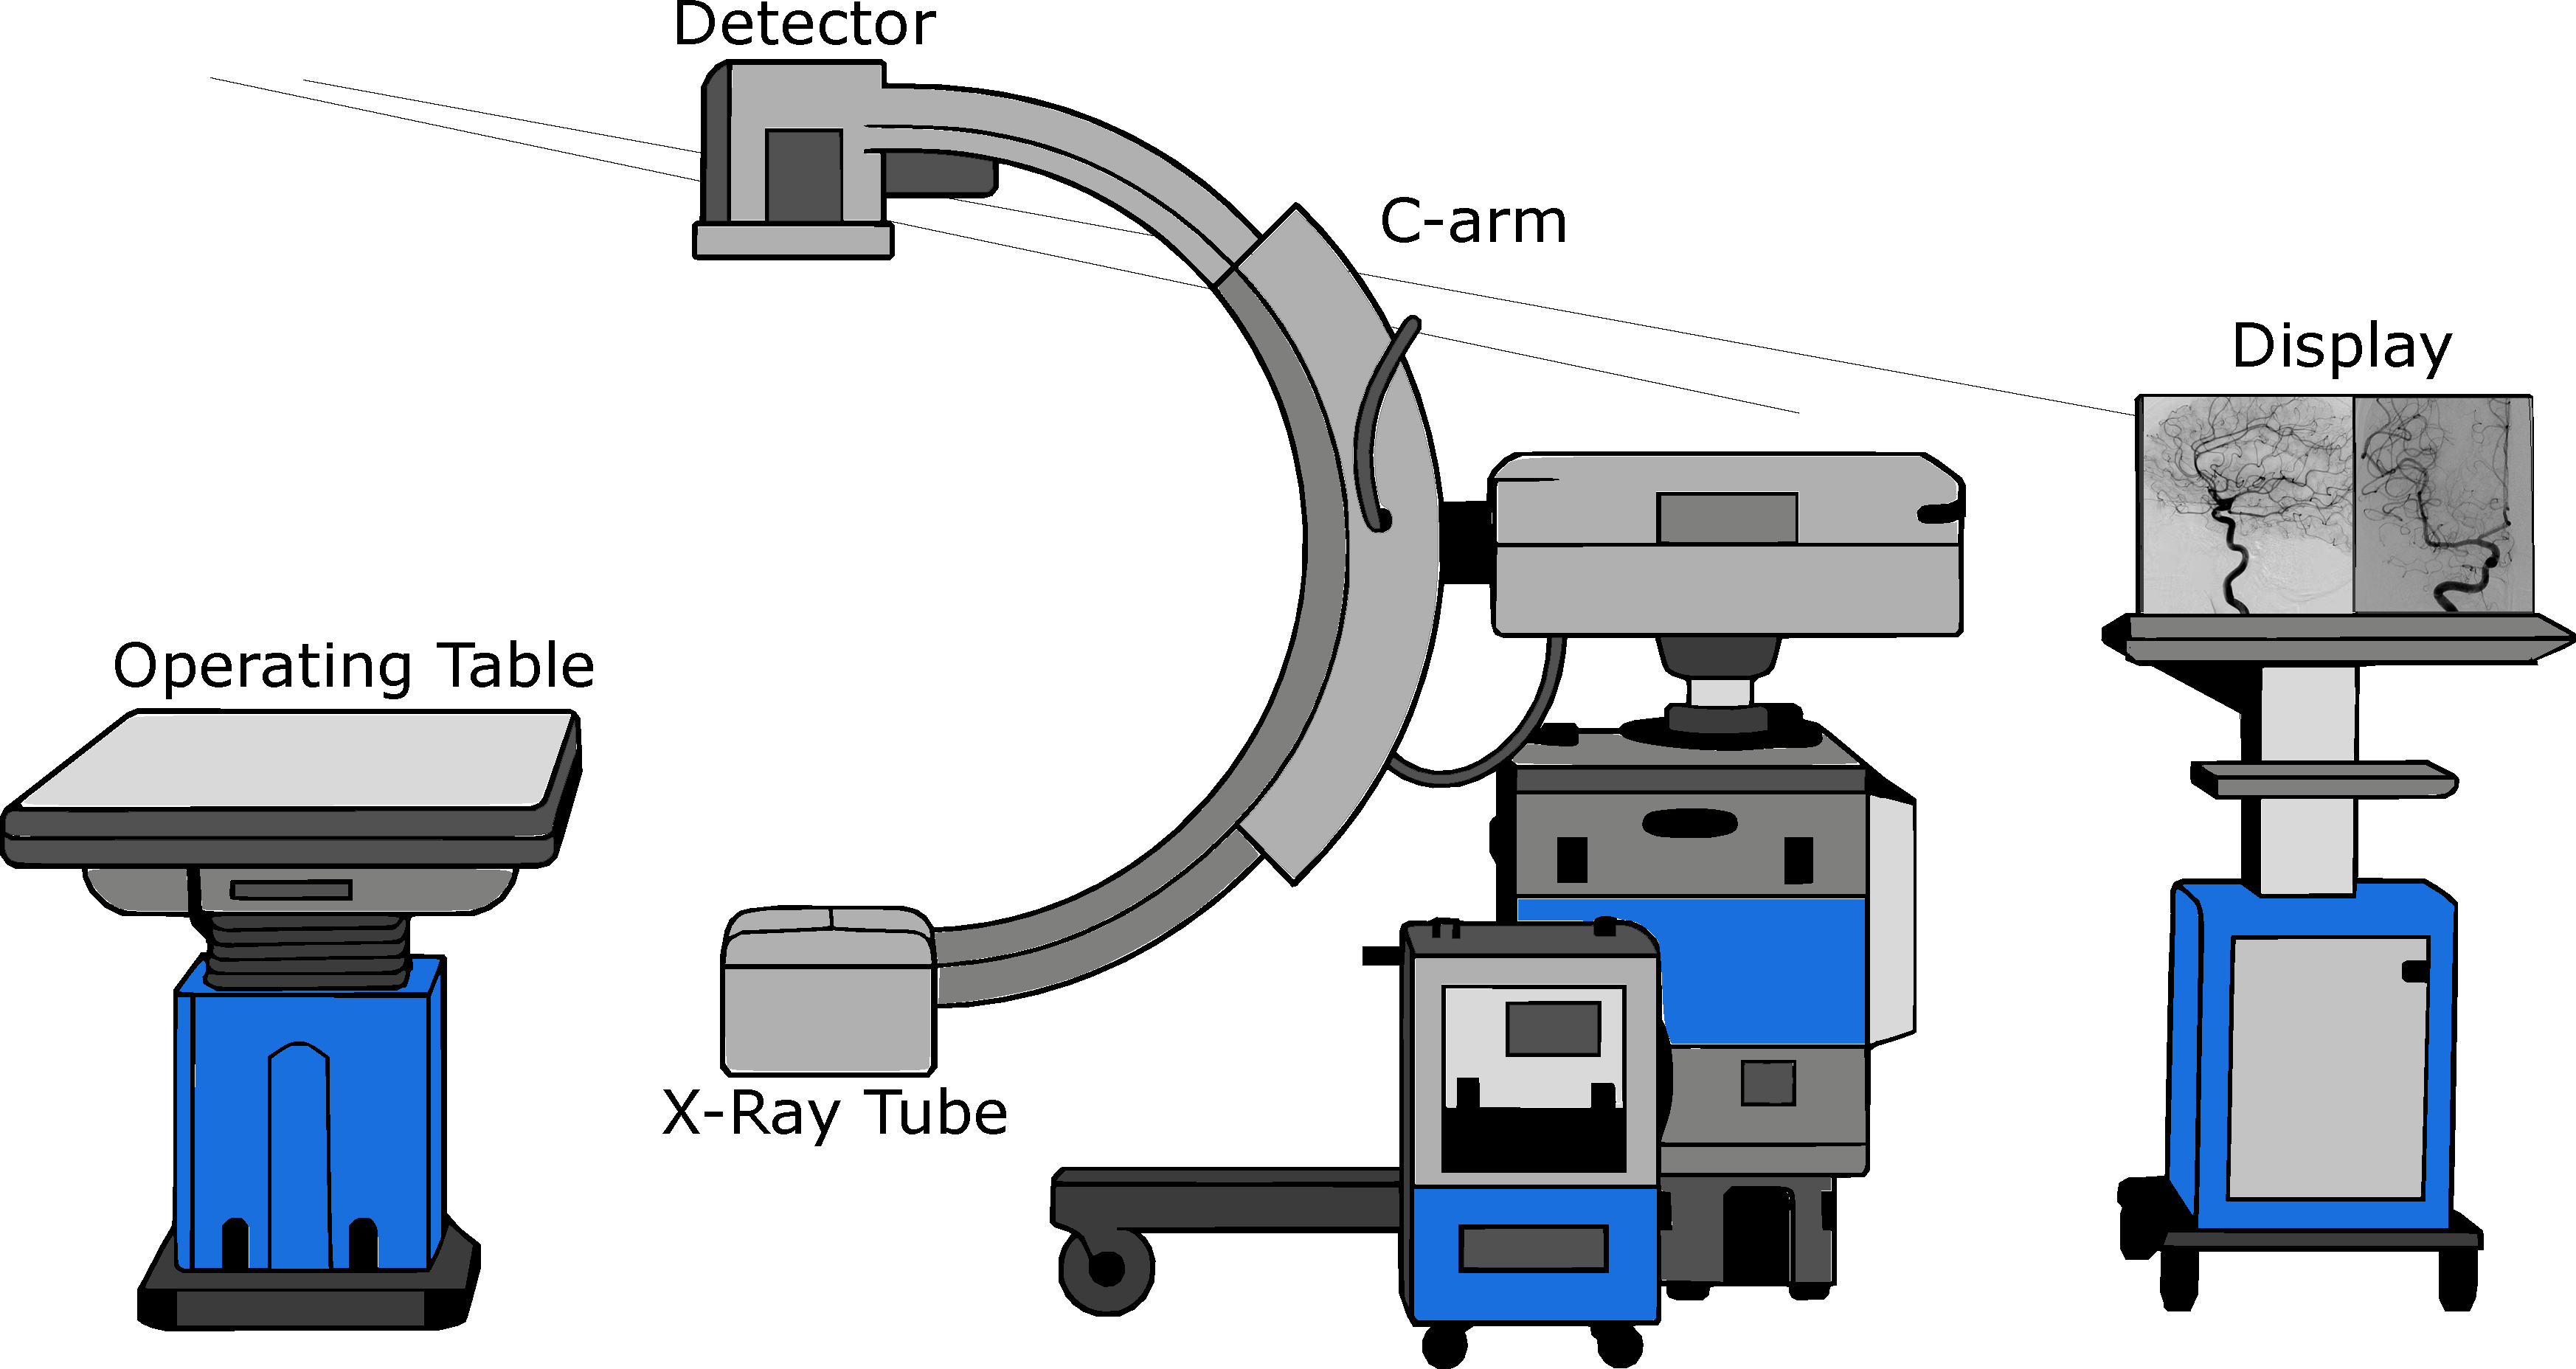
\includegraphics[width=\linewidth]{images/interventional radiology setup.pdf}
 \caption[Interventional Radiology Setup]{Interventional Radiology Setup. The C-arm is positioned in a posteroanterior projection (standard clinical practice) directing the most intense backscatter towards the floor, protecting above-knee radiosensitive organs~\cite{26}. The images shown on the display monitor were reproduced from Refs.~\cite{111,112}.}

 \label{fig:interventional_radiology_setup}
\end{figure}
The conventional IR equipment configuration is illustrated in Fig.~\ref{fig:interventional_radiology_setup}. The X-rays are produced in an X-ray tube by converting the kinetic energy of electrons into electromagnetic radiation. It consists of two electrodes enclosed in a vacuum-sealed glass envelope. The cathode serves as the electron source, while the anode acts as the positive target. When heated by an electric current, the cathode emits electrons via thermionic emission. The number of electrons produced depends on the current passing through the filament. A high potential difference applied between the cathode and the anode accelerates the electrons toward the anode. The total incident energy delivered to the anode is proportional to both the voltage and the current\cite{5,6}.

The X-rays transmitted through the patient strike the image detection system, mounted opposing the X-ray tube on a C-arm gantry. In the standard configuration, the X-ray tube is positioned beneath the patient table and the detector above, capitalising on the anisotropic distribution of scattered radiation to minimise occupational exposure~\cite{21,22}. The detector converts incident X-rays into visible light, which is optically transmitted to a camera system and displayed on a monitor to guide interventions in real-time. For continuous fluoroscopy, a steady tube current is supplied and images are acquired at 30 frames per second to maintain the perception of smooth motion~\cite{16}. Table~\ref{tab:ir_parameters} outlines common technical parameters used in IR procedures \cite{20}.
% Small vertical space after surrounding text
\vspace{1em}

% Manual table title, numbered and added to LoT
\refstepcounter{table}
\label{tab:ir_parameters}
\noindent\textbf{Table~\thetable.} Representative ranges of technical parameters used in IR procedures. Adapted from Ref.~\cite{20}.%
\addcontentsline{lot}{table}{\protect\numberline{\thetable}Representative ranges of technical parameters used in IR procedures.}

% Small space between title and table
\vspace{0.1em}

\begin{table}[H]
  \centering
  \begin{tabular}{>{\raggedright\arraybackslash}p{0.08\textwidth}
                  >{\centering\arraybackslash}p{0.08\textwidth}
                  >{\centering\arraybackslash}p{0.08\textwidth}
                  >{\centering\arraybackslash}p{0.11\textwidth}
                  >{\centering\arraybackslash}p{0.11\textwidth}
                  >{\centering\arraybackslash}p{0.11\textwidth}
                  >{\centering\arraybackslash}p{0.11\textwidth}
                  >{\centering\arraybackslash}p{0.09\textwidth}}

    \toprule
\scriptsize \textbf{Parame\-ter} & \scriptsize \textbf{Peak high voltage} & \scriptsize \textbf{Tube current} & \scriptsize \textbf{Inherent Al filtration} & \scriptsize \textbf{Cu filtration} & \scriptsize \textbf{Pulse duration} & \scriptsize \textbf{Pulse frequency} & \scriptsize \textbf{Scatter Energy} \\

    \midrule
    \scriptsize \textbf{Range}
& \scriptsize 60–120 kV
& \scriptsize 5–1000 mA
& \scriptsize 4.5 mm
& \scriptsize 0.2–0.9 mm
& \scriptsize 1–20 ms
& \scriptsize 1–30 Hz
& \scriptsize 20–100 keV \\
    \bottomrule
  \end{tabular}
\end{table}

 \section{Photon Interaction with Matter}
 \label{sec:Photon Interaction with Matter}
X-rays interact with matter through four physical mechanisms: the photoelectric effect, Compton scattering, Rayleigh dispersion and pair production. The latter two are not relevant in IR~\cite{14}. Therefore, only the photoelectric effect and Compton scattering are considered in detail. Both processes are shown schematically in Fig.~\ref{fig:interaction}.
\subsection{Photoelectric Effect}
The photoelectric effect occurs when an incident photon transfers all of its energy to a bound electron within an atom, resulting in the ejection of the electron from its orbital. This process preferentially involves inner-shell electrons due to their greater electron density. The incident photon energy ($E_0$) is expended to overcome the binding energy of the electron ($E_b$), and any remaining energy is converted into the kinetic energy of the ejected photoelectron ($E_{\text{pe}}$), expressed as~\cite{5,6}:
\begin{equation}
E_{\text{pe}} = E_0 - E_b,\ \text{unit: } [\mathrm{keV}]
\label{eq:photoeletric}
\end{equation}
\indent
The vacancy is filled by an outer electron, with the release of a characteristic X-ray or an Auger electron. When these emissions are reabsorbed within the detector, the total deposited energy equals $E_0$, recorded as the photopeak. As the emissions are monoenergetic, the photopeak would be a Dirac delta. However, and as shown in Fig.~\ref{fig:interaction} (a), the peak has a finite width, set by the energy resolution of the detector and is a property of the instrument~\cite{14}.

The probability of photoelectric interaction is predominant at lower energies ($<$50 keV). It is also dependent on atomic number, increasing with higher-$Z$ materials, which provides contrast in X-ray imaging. As a result, lower-energy X-ray beams produce higher contrast but also increase photon absorption in the patient, leading to a higher dose. In interventional planning, beam quality is therefore optimised to balance image quality and patient dose, as higher photon energies reduce patient absorption but increase the contribution of Compton scattering, leading to greater noise and poorer contrast~\cite{6}.
\begin{figure}[H]
  \centering
  \input{figures/Interaction_with_matter}
  \caption[Photon interactions in IR]{Schematic representation of the photoelectric effect \textbf{(a)} and Compton scattering \textbf{(b)}, and the resulting energy spectrum.}

  \label{fig:interaction}
\end{figure}


\subsection{Compton Scattering}
\label{sec:compton_scattering}
Compton scattering is an inelastic interaction in which an incident photon interacts with a free outer-shell electron, transferring part of its energy. As a result, the electron is ejected as a recoil (Compton) electron. In accordance with the conservation of energy and momentum, the photon is deflected at an angle $\theta$, dependent on the energy transferred. The energy of the scattered photon $E_c$ is described as~\cite{6}:
\begin{equation}
E_c = \frac{E_0}{1 + \frac{E_0}{511} (1 - \cos\theta)},\ \text{unit: } [\mathrm{keV}] \label{eq:compton}
\end{equation}

 Within the detector, all scattering angles are permitted, from $0^\circ$ to $180^\circ$. This creates a Compton continuum, bounded by the two extremes. The maximum energy transfer to the electron occurs at $\theta = 180^\circ$, the Compton Edge (CE). At the same angle, a photon scattered in the surrounding material may enter the detector and be absorbed, forming the backscatter peak shown in Fig.~\ref{fig:interaction} (b)~\cite{14}.

 At photon energies typical of diagnostic radiology, the scattered photon retains most of the initial energy and remains sufficiently energetic to penetrate tissue. Within this energy range, Compton scattering predominates over the photoelectric effect in materials such as soft tissue, water and air. The interaction probability is proportional to the physical density of the material, but it is independent of the atomic number due to the uniform electron density across soft tissues~\cite{5,6}.

\section{Dosimetry Fundamentals}

\subsection{Physical Quantities}
\subsubsection{\emph{KERMA}}
When a beam of indirectly ionizing radiation, such as X-rays, interacts with matter, it transfers energy to charged particles within the medium. The total energy transferred ($\varepsilon_{tr}$) within a volume, $V$, is defined as \cite{12}:
\begin{equation}
\varepsilon_{tr} = (R_{in})_u - (R_{out})_u^{\text{nonr}} + \sum Q,\ \text{unit: } [\mathrm{J}]
\label{eq:energy_transferred}
\end{equation}
\noindent where \((R_{\text{in}})_u\) and \((R_{\text{out}})_u\) are the radiant energies of uncharged particles entering and leaving the volume, respectively, excluding secondary radiative emissions. \(\sum Q\) represents changes in rest mass energy within \(V\).

The dosimetric quantity \emph{KERMA} (Kinetic Energy Released in MAtter) quantifies the initial kinetic energy transferred to char\-ged particles, per unit mass, regardless of where and how that energy is spent \cite{6,12}:
\begin{equation}
KERMA = \frac{d\varepsilon_{tr}}{dm},\ \text{unit: } \left[\frac{\mathrm{J}}{\mathrm{kg}}\right] \text{ or } [\mathrm{Gy}]
\label{eq:kerma}
\end{equation}
\subsubsection{Absorbed Dose}
Absorbed dose ($D$) incorporates all subsequent energy deposition mechanisms such as radiative losses, e.g. \emph{Bremsstrahlung}. The total deposited energy (\( \varepsilon \)) includes the energy balance defined in Eq. \ref{eq:energy_transferred}, along with all contributions from charged particles, per unit mass at a point of interest. $D$ is used to quantify the effects of radiation and is expressed as \cite{11,12}:
\begin{equation}
D = \frac{d\varepsilon}{dm},\ \text{unit: } [\mathrm{Gy}]
\label{eq:absorbed_dose}
\end{equation}

\subsubsection{Exposure}
Exposure ($X$) is the earliest defined dosimetric quantity and applies to photon interactions in air. It measures the amount of electric charge, \(dQ\), produced by ionization in a given mass of dry air \cite{12}:
\begin{equation}
X = \frac{dQ}{dm},\ \text{unit: } \left[\frac{\mathrm{C}}{\mathrm{kg}}\right]
\label{eq:exposure}
\end{equation}

Exposure is directly related to the collision component of \emph{KERMA}, (\(K_{col}\)). \(K_{col}\) represents the fraction of energy transferred that is deposited through ionization and excitation, excluding radiative losses. In fact, a connection between $X$ and \(K_{\text{col}}\) can be established through the quantity \(\overline{W}_{\text{air}}\), defined as the mean energy required to produce an ion pair in dry air (\(\overline{W}_{\text{air}} = 33.97~\mathrm{J/C}\)):
\begin{equation}
K_{\text{col, air}} = \overline{W}_{\text{air}} \cdot X = 33.97 \cdot X,\ \text{unit: } [\mathrm{Gy}]
\label{eq:kcair_exposure}
\end{equation}
\noindent
In practice, \(K_{\text{col, air}}\) is commonly referred to as \emph{air KERMA} and is used to describe the output of an X-ray tube, as it can be measured directly in free air \cite{11}.

\subsection{Protection Quantities}
Radiation effects on humans vary due to differences in bio\-logical response and are classified as either stochastic or deterministic. Deterministic effects (Fig.~\ref{fig:effects}~(a)), inclu\-ding development of cataracts or skin erythema, have a threshold dose and increase in severity with higher exposure.  Stochastic outcomes (Fig.~\ref{fig:effects}~(b)), such as cancer, occur statistically, with the probability increasing with dose but without a threshold. To reflect these probabilistic biological responses, additional weighting factors for radiation type and tissue radiosensitivity must be considered. Thus, two protection-related quantities, equivalent dose ($H$) and effective dose~($E$), are derived from absorbed dose~\cite{13,14}.
\begin{figure}[H]
  \centering
  \tikzset{every picture/.style={line width=0.75pt}}

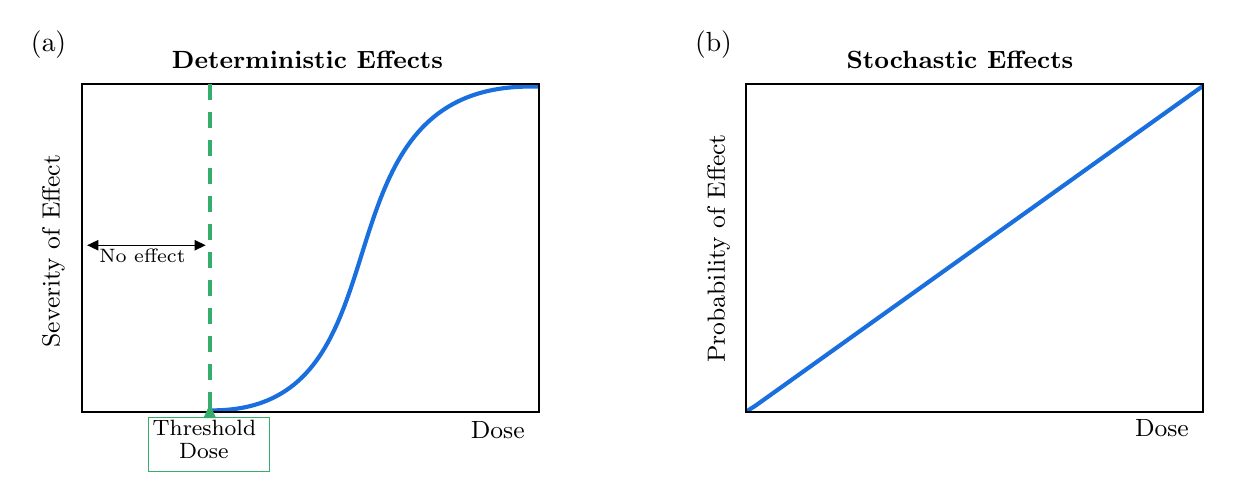
\begin{tikzpicture}[x=0.75pt,y=0.75pt,yscale=-1,xscale=1]

%Straight Lines [id:da7730700763729692] 
\draw [color={rgb, 255:red, 26; green, 111; blue, 223}  ,draw opacity=1 ][line width=1.5]    (599.76,48.96) -- (385.01,202.42) -- (380.42,205.43) ;
%Curve Lines [id:da8629624283311327] 
\draw [color={rgb, 255:red, 26; green, 111; blue, 223}  ,draw opacity=1 ][line width=1.5]    (121.47,205.11) .. controls (198.34,206.12) and (184.08,114.95) .. (221.47,71.53) .. controls (233.7,57.34) and (251.44,48.25) .. (279.69,49.16) ;
%Shape: Rectangle [id:dp07258514804006644] 
\draw  [line width=0.75]  (60,48) -- (280,48) -- (280,206) -- (60,206) -- cycle ;
%Straight Lines [id:da09166760913517435] 
\draw [color={rgb, 255:red, 55; green, 173; blue, 107}  ,draw opacity=1 ][line width=1.5]  [dash pattern={on 5.63pt off 4.5pt}]  (121.38,47.92) -- (121.38,206.32) ;
%Straight Lines [id:da3468358858445303] 
\draw    (65.4,125.56) -- (116.52,125.56) ;
\draw [shift={(119.52,125.56)}, rotate = 180] [fill={rgb, 255:red, 0; green, 0; blue, 0 }  ][line width=0.08]  [draw opacity=0] (5.36,-2.57) -- (0,0) -- (5.36,2.57) -- cycle    ;
\draw [shift={(62.4,125.56)}, rotate = 0] [fill={rgb, 255:red, 0; green, 0; blue, 0 }  ][line width=0.08]  [draw opacity=0] (5.36,-2.57) -- (0,0) -- (5.36,2.57) -- cycle    ;
%Shape: Rectangle [id:dp4467912586395093] 
\draw  [color={rgb, 255:red, 55; green, 173; blue, 107}  ,draw opacity=1 ] (91.8,208.57) -- (150.3,208.57) -- (150.3,234.63) -- (91.8,234.63) -- cycle ;
%Shape: Triangle [id:dp7577642747879886] 
\draw  [color={rgb, 255:red, 55; green, 173; blue, 107}  ,draw opacity=1 ][fill={rgb, 255:red, 55; green, 173; blue, 107}  ,fill opacity=1 ] (121.5,202.71) -- (124.14,208.56) -- (118.85,208.56) -- cycle ;
%Shape: Rectangle [id:dp10920079476550804] 
\draw  [line width=0.75]  (380,48) -- (600,48) -- (600,206) -- (380,206) -- cycle ;

% Text Node
\draw (102,31) node [anchor=north west][inner sep=0.75pt]  [font=\small] [align=left] {\textbf{Deterministic Effects}};
% Text Node
\draw (67,126) node [anchor=north west][inner sep=0.75pt]  [font=\small] [align=left] {{\scriptsize No effect}};
% Text Node
\draw (427,31) node [anchor=north west][inner sep=0.75pt]  [font=\small] [align=left] {\textbf{Stochastic Effects}};
% Text Node
\draw (246,209) node [anchor=north west][inner sep=0.75pt]  [font=\small] [align=left] {Dose};
% Text Node
\draw (566,208) node [anchor=north west][inner sep=0.75pt]  [font=\small] [align=left] {Dose};
% Text Node
\draw (39.5,176) node [anchor=north west][inner sep=0.75pt]  [font=\small,rotate=-270] [align=left] {Severity of Effect};
% Text Node
\draw (360,183.33) node [anchor=north west][inner sep=0.75pt]  [font=\small,rotate=-270] [align=left] {Probability of Effect};
% Text Node
\draw (92.7,208.5) node [anchor=north west][inner sep=0.75pt]  [font=\small] [align=left] {{\footnotesize Threshold}};
% Text Node
\draw (105.45,219.83) node [anchor=north west][inner sep=0.75pt]  [font=\small] [align=left] {{\footnotesize Dose}};
% Text Node
\draw (34,21) node [anchor=north west][inner sep=0.75pt]   [align=left] {(a)};
% Text Node
\draw (354,21) node [anchor=north west][inner sep=0.75pt]   [align=left] {(b)};
\end{tikzpicture}

  \caption[Deterministic and stochastic effets.]{\textbf{(a)} Deterministic effects exhibit a threshold dose below which no effect occurs. Above the threshold, severity increases with dose. Thresholds are expressed in Gy (absorbed dose) as deterministic effects depend only on how much energy is deposited.
    \textbf{(b)} Stochastic effects have no threshold; the probability of occurrence increases with dose, but severity is independent of exposure. The individual either develops the condition or not \cite{13}.}

  \label{fig:effects}
\end{figure}


\subsubsection{Equivalent Dose}
The stochastic effects of radiation depend on the type of particles involved, as they interact with matter in distinct ways, exhibiting different patterns of ionization along their paths~\cite{12}. This variation is described by the linear energy transfer (LET) function, which represents the rate at which energy is deposited along a particle’s trajectory through a medium. Low-LET radiation produces ionization over longer paths, whereas high-LET radiation transfers energy more densely over shorter distances, enhancing its potential for biological damage per unit of absorbed dose~\cite{6}.

To account for these differences in LET, the International Commission on Radiological Protection (ICRP) introduced the concept of equivalent dose. This measure applies an empirical and dimensionless radiation weighting factor, $w_R$, to the absorbed dose, to reflect the relative biological effectiveness of different types of radiation~\cite{6,14}:

\begin{equation}
H_T = \sum_R D_{T,R} \cdot w_R,\ \text{unit: } [\mathrm{Sv}]
\label{eq:equivalent_dose}
\end{equation}

\noindent The sievert (Sv) is dimensionally equivalent to joules per kilogram (J/kg) and gray (Gy), but specifically used for radiological protection to distinguish it from the physical quantity $D$~\cite{6}.

As shown in Table \ref{tab:wr_factors}, fast electrons, X-rays and $\gamma$-rays have a weighting factor $w_R$ of one, meaning that absorbed dose and equivalent dose are numerically equal~\cite{14}. In contrast, $\alpha$ particles have a $w_R$ of 20 due to their higher ionization density. Thus, $\alpha$ particles can produce the same biological outcome as X-rays at only 5\% of the absorbed dose~\cite{13,14}.

% Right before the table environment
% Small vertical space after surrounding text
\vspace{1em}
% Manual table title, numbered and added to LoT
\refstepcounter{table}
\label{tab:wr_factors}
\noindent\textbf{Table~\thetable.} Radiation weighting factors. Adapted from Ref.~\cite{15}.%
\addcontentsline{lot}{table}{\protect\numberline{\thetable}Radiation weighting factors.}


\vspace{0.1em} % Small space between title and table
\begin{table}[H]
\centering
\begin{tabular}{c c}
\toprule
\textbf{Radiation type} & \textbf{Radiation weighting factor, $w_R$} \\
\midrule
X-rays, $\gamma$-rays and Electrons & 1 \\
Protons & 2 \\
$\alpha$ and Heavy Particles & 20 \\
Neutrons &
\begin{minipage}[c][3.5cm][c]{0.4\textwidth}
\centering
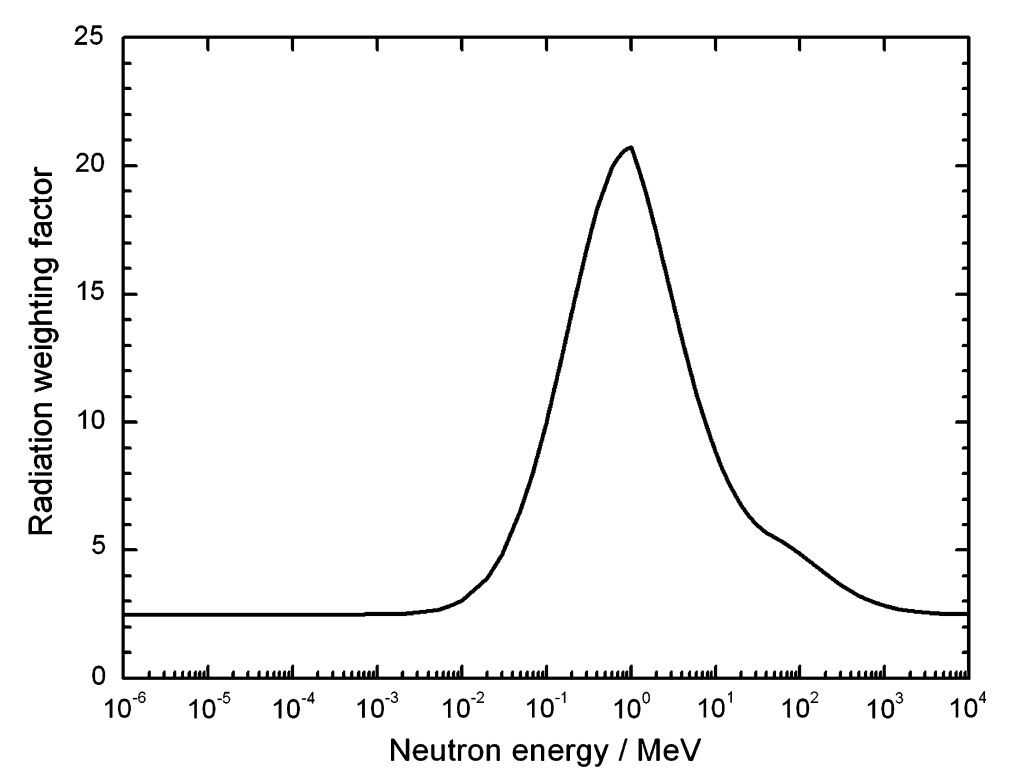
\includegraphics[height=3cm]{images/neutron.jpg} \\
\footnotesize {Continuous function of neutron energy}
\end{minipage} \\
\bottomrule
\end{tabular}

\end{table}

\subsubsection{Effective Dose}
Effective dose extends the concept of equivalent dose by incorporating tissue weighting factors, $w_T$. These factors quantify the relative contribution of specific organs and tissues to the overall radiation detriment, and are represented in Table \ref{tab:wt_factors}. The values are derived from epidemiological and radiobiological data and reflect averaged population risk, making $E$ a comparative metric rather than an indicator of individual risk. Effective dose is defined as the sum of the equivalent doses received by individual organs and tissues, each weighted by its respective factor~\cite{6,13,14}:

\begin{equation}
E = \sum_T H_T \cdot w_T,\ \text{unit: } [\mathrm{Sv}]
\label{eq:effective_dose}
\end{equation}

% Small vertical space after surrounding text
\vspace{1em}

% Manual table title, numbered and added to LoT
\refstepcounter{table}
\label{tab:wt_factors}
\noindent\textbf{Table~\thetable.} Tissue weighting factors for each organ/tissue. Adapted from Ref.~\cite{15}.%
\addcontentsline{lot}{table}{\protect\numberline{\thetable}Tissue weighting factors for each organ/tissue.}

% Small space between title and table
\vspace{0.1em}

\begin{table}[H]
  \centering
  \begin{tabular}{p{0.58\textwidth} c c}
    \toprule
    \textbf{Tissues and Organs} & \textbf{Weighting Factor,$w_T$} & \textbf{$\sum w_T$} \\
    \midrule
    Red bone marrow, Colon, Lung, Stomach, Breast, Remaining tissues* & 0.12 & 0.72 \\
    Gonads & 0.08 & 0.08 \\
    Bladder, Esophagus, Liver, Thyroid & 0.04 & 0.16 \\
    Bone surface, Brain, Salivary glands, Skin & 0.01 & 0.04 \\
    \midrule
    & \textit{Total} & \textbf{1.00} \\
    \bottomrule
  \end{tabular}

  \vspace{0.3em}
  {\footnotesize *Adrenals, Extrathoracic region,
Gall bladder, Heart, Kidneys, Lymphatic nodes, Muscle, Oral
mucosa, Pancreas, Prostate, Small intestine, Spleen, Thymus, Uterus/cervix}
\end{table}
\subsection{Operational Quantity}
In operational dosimetry, equivalent and effective dose cannot be measured directly~\cite{13}. Personal dosimetry is the applied science of using individual monitoring devices to estimate dose from occupational exposure. These devices are calibrated in terms of the personal dose equivalent, $H_p(d)$, defined as the dose equivalent in soft tissue at a depth $d$~mm beneath a specified point on the body and is expressed in Sv. At 10 mm, $H_p(10)$ is used to estimate effective dose from deeply penetrating radiation and is the principal quantity for assessing whole-body exposure. Dosimeters intended to measure Hp(10) are calibrated using reference radiation qualities defined in ISO 4037-1~\cite{113}. During calibration, the dosimeter is mounted on a polymethyl methacrylate (PMMA) phantom, and the field is characterized in terms of \emph{air KERMA}. For each radiation energy $E$ and angle of incidence $\alpha$, the International Commission on Radiation Units and Measurements (ICRU) provides conversion coefficients $h_{pK}(10; E, \alpha)$, which relate \emph{air KERMA} to $H_p(10)$~\cite{ICRU53}:
\begin{equation}
H_p(10) = h_{pK}(10; E, \alpha)\cdot K_{\mathrm{air}}, \quad [\mathrm{Sv}]
\label{eq:hp10}
\end{equation}

The same calibration approach applies to the assessment of equivalent dose, for which shallower depths are used. At 0.07 mm, $H_p(0.07)$ is used to assess dose to the skin from weakly penetrating radiation, and at 3 mm, $H_p(3)$  has been proposed specifically for the lens of the eye~\cite{13}.

\section{Occupational Exposure}
As previously mentioned, at the photon energies typical of fluoroscopy (recall Table~\ref{tab:ir_parameters}), the Compton effect predominates, degrading image quality and generating scattered radiation throughout the room \cite{6,23}. This stray radiation is the main source of occupational exposure for staff \cite{24}. From a dosimetric perspective, characterising the IR settings is inherently challenging due to the variability of parameters that influence radiation output and scatter distribution \cite{30}. In general, exposure to staff is proportional to the dose received by the patient \cite{21}. Tube voltage and current are adjusted based on patient size and anatomy during procedure planning, which in turn influence the amount of scatter produced \cite{30,31}. In addition, FOV and beam filtration also play a role, though their effects are not linear and highly dependent on scatter geometry \cite{32}. Beyond equipment settings, procedural complexity and operator technique contribute to variations in staff exposure. Advanced or prolonged interventions typically require longer fluoroscopy times, more image acquisitions, and non-standard projections \cite{30}. Operator experience has been shown to significantly reduce exposure through more efficient techniques, reduced reliance on fluoroscopy, and better positioning practices \cite{33}.

To illustrate scatter behaviour in a real clinical context, Fig.~\ref{fig:scatter} presents an isodose map, at chest height, generated during a fluoroscopically guided hip replacement procedure, and highlights the locations typically occupied by staff \cite{34}. The image reveals an asymmetric scatter pattern, with notably higher intensities recorded opposite to the position of the C-arm. The referenced study also reported lower dose levels on the side opposite the patient table, where equipment provides partial shielding. Although the inverse square law does not perfectly apply in the clinical environment \cite{35} due to scattering within the patient and surrounding structures, a general decrease in dose rate with increasing distance was still evident \cite{34}. This reaffirms the protective effect of physical separation from the source \cite{36}.
\begin{figure}[H]
  \centering
  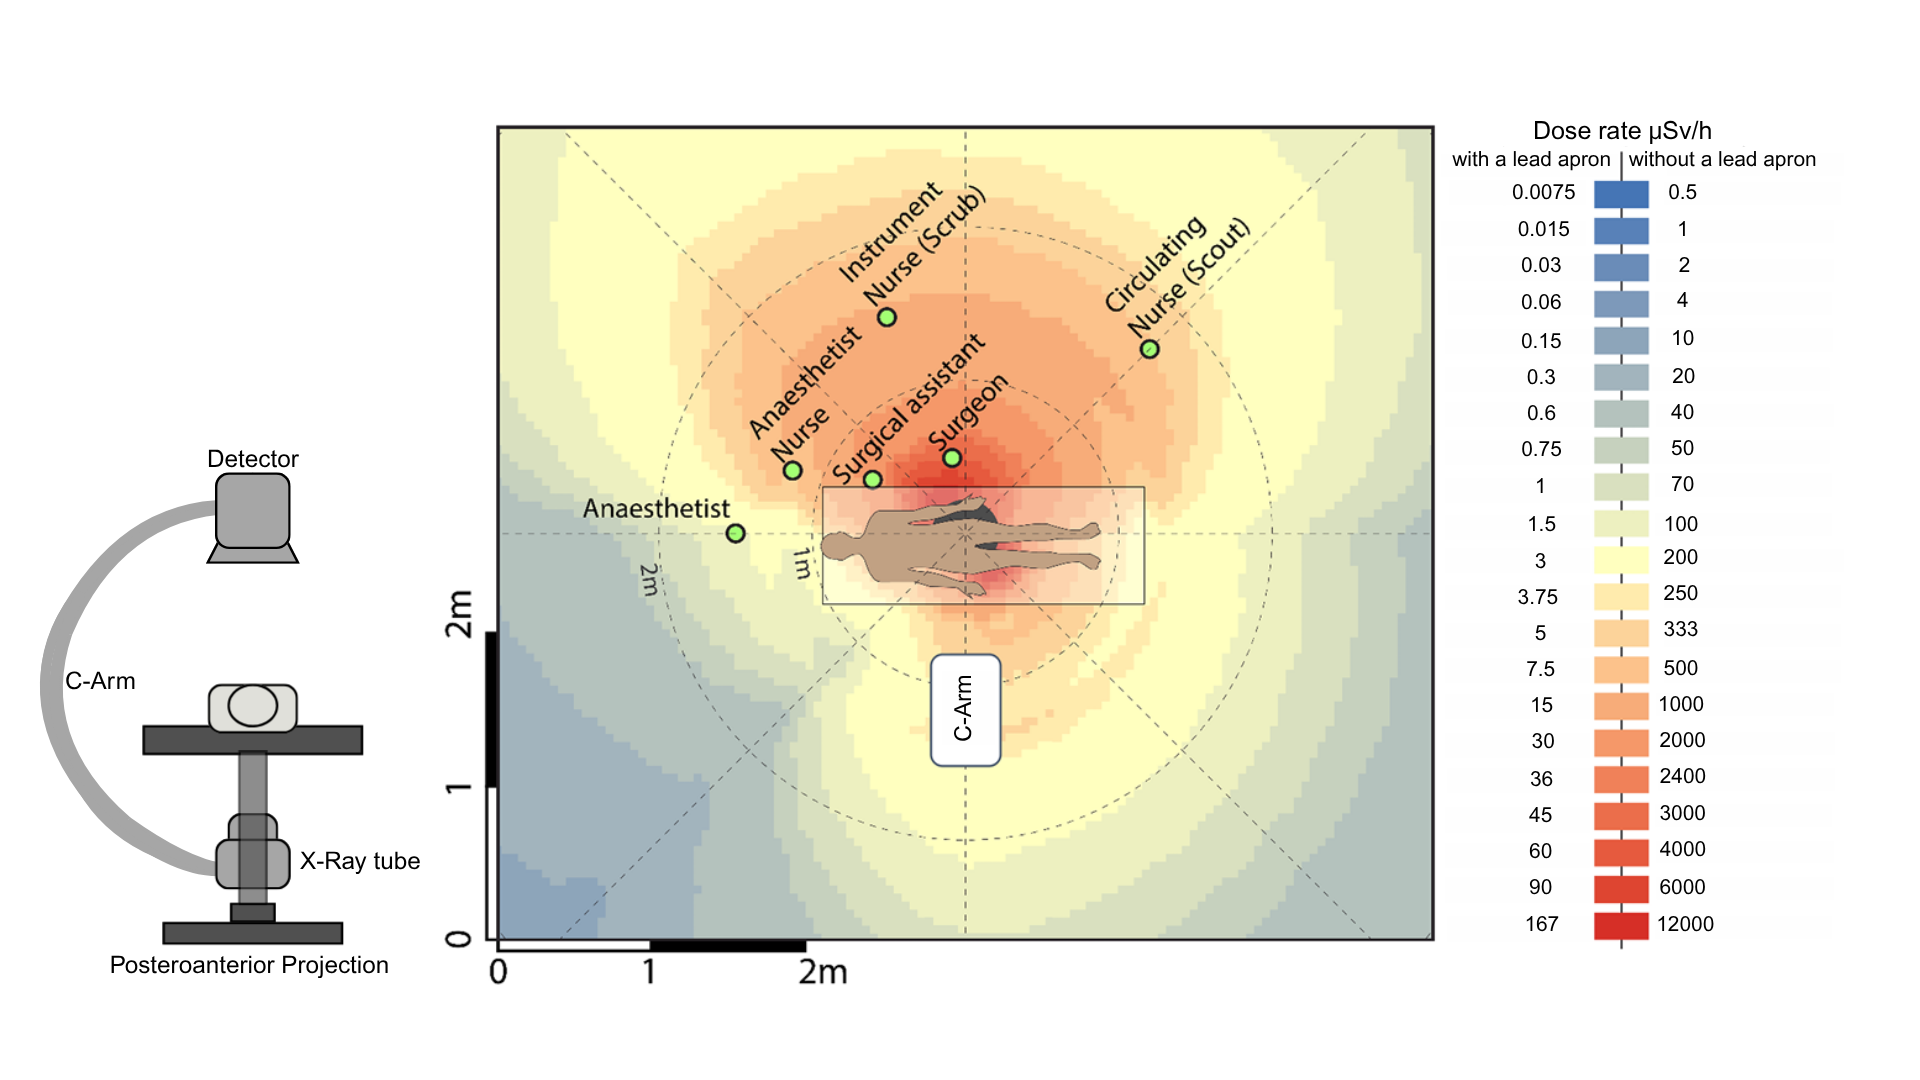
\includegraphics[width=\linewidth]{images/dose rates.png}
  \caption[Scatter radiation distribution in IR environment.]{Isodose map of scatter radiation during a fluoroscopically guided hip replacement procedure. Acquisition parameters included 77~kVp, 20.6~mA, 32.1~s of fluoroscopy time, and a pulse rate of 15~fps. Dose rates were measured using an active dosimeter at multiple positions around the phantom and linearly interpolated to generate the map. Values incorporating shielding (right scale) were estimated using theoretical models. Measurements are documented at chest level. The image was adapted from Ref.~\cite{34}. Although the C-arm configuration was not explicitly reported, a posteroanterior projection (left icon) was inferred based on findings from Ref.~\cite{35}.
  }

  \label{fig:scatter}
\end{figure}

Protection against cumulative exposure requires consistent application of shielding practices \cite{37}. Shielding is implemented at multiple levels, including structural room design, fixed barriers, and mobile shields, which contribute to protecting helping staff \cite{38} and sensitive areas such as the head and eyes, respectively~\cite{39}. However, personal protective equipment remains the most reliable and controllable form of protection. According to ICRP recommendations, all staff should wear lead aprons, along with thyroid shields, during fluoroscopic procedures \cite{37,39}. Most aprons have a lead thickness range of 0.35 to 0.5~mm, with 0.5~mm reducing scattered radiation by over 90\% \cite{37}. To be effective, aprons must fit properly, and facilities should be encouraged to invest in a variety of sizes to ensure proper coverage and comfort \cite{38,40}. Thyroid shields are manufactured with a lead equivalence of 0.5~mm and have been reported to reduce exposure to the gland by approximately 50\% \cite{41}. %Their use is particularly advised for staff who receive monthly collar readings above 4~mSv and are under 40 years of age, due to the increased risk of thyroid cancer \cite{42}.
Lead glasses are also available but remain underutilised. As the second most effective protective measure after ceiling-suspended shields, these glasses are available in various frame designs and thicknesses ranging from 0.35 to 0.75~mm. %Their protective benefit, however, depends greatly on the positioning of the operator’s head in relation to the patient during procedures \cite{40}.

 The effectiveness of these protective measures is ultimately verified against the annual occupational dose limits recommended by the ICRP, summarised in Table \ref{tab:occupational_dose_limits}. These limits are not an absolute safety threshold but rather boundaries beyond which cumulative exposures are no longer considered justified~\cite{13}. For instance, the $E$ limit for radiation workers is set at 20~mSv per year, averaged over five years, with an upper limit of 50~mSv in any single year \cite{15}.




\vspace{1em}

\refstepcounter{table}
\label{tab:occupational_dose_limits}
\noindent\textbf{Table~\thetable.} ICRP occupational dose limits. Adapted from Refs.~\cite{15,44}.%
\addcontentsline{lot}{table}{\protect\numberline{\thetable}ICRP occupational dose limits.}

\vspace{0.1em}


\begin{table}[H]
\centering
\renewcommand{\arraystretch}{1.4}
\setlength{\tabcolsep}{8pt}
\begin{tabular}{
  >{\centering\arraybackslash}m{0.22\textwidth}
  >{\centering\arraybackslash}m{0.33\textwidth}
  >{\centering\arraybackslash}m{0.33\textwidth}}
\toprule
\multicolumn{2}{m{0.55\textwidth}}{\centering\textbf{Protection Quantity}} & \textbf{Annual Permissible Dose} \\
\midrule
\multicolumn{2}{m{0.55\textwidth}}{
  \centering\textbf{Effective Dose}
} &
\begin{minipage}[c][3.5\baselineskip][c]{\linewidth}
\centering
20 mSv per year averaged over 5 years \\
(no single year exceeding 50 mSv)
\end{minipage} \\
\midrule
\multirow{3}{=}{\textbf{Equivalent Dose}}
& Lens of the Eyes & 20 mSv \\
& Thyroid Gland & 300 mSv \\
& Individual Organs (excluding the eye), Skin and Extremity & 500 mSv \\
\bottomrule
\end{tabular}
%\caption{Annual permissible dose limits for various protection quantities.}
\end{table}

As previously introduced, currently, compliance with occupational dose limits in IR is verified through routine monitoring using passive dosimeters worn by staff over predefined time intervals. The most common devices are thermoluminescent dosimeters and optically stimulated luminescence dosimeters. Both operate by trapping energy when exposed to ionising radiation, which is later released as light when stimulated under controlled conditions. The intensity of the emitted light is proportional to the amount of absorbed radiation \cite{11}. These devices measure the previously discussed quantity $H_p(10)$. While $H_p(10)$ can serve as an approximation of effective dose under conditions of uniform whole-body exposure, this does not reflect the typical environment in IR, as described \cite{64}. When a single dosimeter is used, placement beneath the lead apron tends to underestimate $E$ due to shielding, while positioning it above may overestimate it~\cite{30}. To improve accuracy, the ICRP recommends a dual dosimetry approach. In this method, one dosimeter is worn underneath the protective apron between the waist and chest to record the attenuated exposure to shielded tissues ($H^u$). The second device is placed at collar level outside the apron to monitor exposure to unshielded regions ($H^o$). An effective dose estimate is then calculated by applying a linear combination of these two measurements \cite{65}:

\begin{equation}
E = \alpha H^u + \beta H^o,\ \text{unit: } [\mathrm{Sv}]
\label{eq:dual_dosimetry}
\end{equation}

However, there is currently no global consensus on the value of both weighting factors, $\alpha$ and $\beta$ \cite{65}. Over 14 different algorithms have been reported in the literature, most of which overestimate $E$. Despite this variability, double dosimetry remains more accurate than single-dosimeter methods \cite{66}.

The major limitation of passive dosimeters lies in their inability to provide dose information in real-time. These devices are typically read at monthly intervals \cite{67}, which prevents identification of excessive exposures or deviations from standard operating conditions in time. As a result, opportunities for real-time corrective action are lost, and staff may remain unaware of elevated exposure levels until the data can be reviewed retrospectively \cite{46,68}. In this context, active personal dosimeters (APDs) have emerged as a complementary solution. APDs are not intended to replace passive dosimeters, which remain the standard for legal dose documentation. By providing real-time feedback on dose rate, APDs support adherence to the ALARA principle by enabling immediate adjustments to operator behaviour or shielding practices \cite{2,3}.

\section{Real-Time Dosimetry}
The concept of real-time radiation monitoring in occupational settings was first established through the use of APDs, which have been widely adopted in the nuclear industry as a standard safety practice \cite{69}. However, it was only within the last 15 years that their use in IR began to be critically evaluated \cite{2,38,69,70}. As previously discussed, the IR environment is characterised by pulsed radiation, lower photon energies, and predominantly scattered fields, which differ significantly from the conditions under which the APDs available at the time were originally developed \cite{70}. Although several studies \cite{20,69,70} explored the possibility of adapting existing devices for IR, it was Sánchez \emph{et al}. \cite{2}, working as part of an early development initiative at Philips, who introduced the first APD specifically engineered for interventional use. Unlike existing APDs that provided exclusively auditory feedback, this prototype included a visual interface displaying real-time dose data to staff in the procedure room. It became the first generation of the DoseAware system, which started being distributed commercially in 2010 \cite{71}. Later, Philips and Unfors RaySafe signed a joint development agreement in 2012 and, in 2017, the third-generation system, RaySafe i3, was introduced at the European Congress of Radiology \cite{76}.

The device features a silicon solid-state diode \cite{72}, integrated into an invididual wearable bagde with wireless capabilities, transmitting scattered dose information to a data collection unit at a one second rate. Detected dose values are displayed on an in-room monitor as both numerical data and a bar graph. Each badge is represented individually, with exposure levels indicated using a colour-coded scheme (green, yellow, and red) corresponding to increasing dose rates~\cite{2}.
The operational photon energy range of the system is N40--N150 for X- and $\gamma$-radiation. The relative measurement uncertainty is approximately 10\% for dose rates in the range of 40--150~$\mu$Sv/h and 20\% for dose rates between 150--300~$\mu$Sv/h. The system has been shown to correlate well with legal-for-record passive dosimeters, typically overestimating $H_{\mathrm{p}}(10)$ by 5--15\%.

The collaboration between Philips and RaySafe enabled the integration of badge-derived data into dedicated software platforms, such as Dose Viewer and Dose Manager \cite{81}. These platforms support retrospective analysis by allowing users to access, export, and manage individual dose histories, as well as aggregate exposure data across teams or departments. RaySafe i3 is currently priced at around 27,000\euro~\cite{79}, which raises concerns about cost. Individual APD units are expensive, making it difficult for most imaging departments to provide them for all staff. In addition, current systems do not support extremity monitoring, such as for the eyes or hands \cite{80}.

\subsection{Reported Benefits}
The development and clinical integration of the APDs described above enabled structured evaluation of their practical impact in IR. Since their introduction, a number of studies have compared conditions with and without real-time feedback~\cite{4,68,72,82,83,85,86,87,88,114,115,116}. A common finding is a general decrease in staff dose when feedback is available. This effect appears across various professional roles, though the degree of reduction can vary. In a study led by Baumann \emph{et al}~\cite{86} dose reduction was observed in almost every staff group~\cite{86}. Further analysis reveals a pattern seen across multiple studies, where the most significant reductions are recorded in the main radiologist, who is positioned closest to the patient. In some studies, this group was the only one to show a statistically significant change in radiation exposure~\cite{72,86,87,88}. This may be explained by findings from Baumgartner \emph{et al}\ \cite{72}, which showed that procedural contexts associated with higher radiation exposure tend to demonstrate the most pronounced reductions following the introduction of APDs \cite{72}. This is consistent with reports that the effectiveness of APDs depends on baseline conditions. Operators who initially demonstrated poor radiation safety habits were able to significantly reduce their dose after the introduction of APDs through simple corrective actions. In contrast, those already practising good protection strategies had less room to improve and showed minimal change \cite{82,87,115}. These baseline variations are also associated with the operator’s level of experience, as discussed in section~1.4, and were recently studied by Koch \emph{et al}~\cite{83}. A pronounced decrease in dose was registered among the least experiences group, while operators with over ten years of experience show, in this case, even a slight increase in dose. Experienced operators may rely on ingrained habits and confidence in their technique, whereas less experienced users appear to adjust more readily when confronted with live feedback \cite{83}. It has been reported that younger operators tend to show less concern for radiation safety \cite{89}. These results suggest that APDs may be especially valuable as educational tools for junior staff, helping them build good radiation safety practices \cite{83}.

Consistent with these findings, James \emph{et al}~\cite{115}, reported a reduction in red events over time. They argued that, while these events serve as prompts for immediate dose adjustment, they also function as a reflective tool for operators. This enables professionals to identify specific maneuvers, projection angles, and procedural choices associated with increased radiation exposure. Consequently, such practices can be replaced by lower-exposure alternatives and operators can adopt safer procedural habits more permanently. Ultimately, it also contributes to a reduction in radiation dose to the patient~\cite{115,116}.

Other staff members, including nurses and technicians, also benefited from dose reductions \cite{82,83,85,86,88,115}. In these cases, it was primarily attributed to individual awareness and simple adjustments, such as changes in positioning. Some studies further emphasised the collaborative value of these systems, noting that when all staff members wear APDs with visible displays, teams can collectively monitor exposure. This practice creates an environment of mutual accountability, where individuals not only adjust their own behaviour but also remain aware of their colleagues’ exposure, promoting safer team dynamics \cite{86,87,115}.

\newpage
%%%%%%%%%%%%%%%%%%%%%%%%%%%%%%%%%%%%%%%%%%%%%
%%% Chapter 2: DORI - Hardware Development
%%%%%%%%%%%%%%%%%%%%%%%%%%%%%%%%%%%%%%%%%%%%%
\chapter{Hardware Development}
\label{chapter:hardware_development}
This chapter describes the development of the DORI (\textit{DOs\'imetro para Radiologia de Interven\c{c}\~ao}) prototype, designed in response to the previously identified limitations. The conceptual design of the system is shown in Fig.~\ref{fig:DORI}.
\begin{figure}[H]
  \centering
  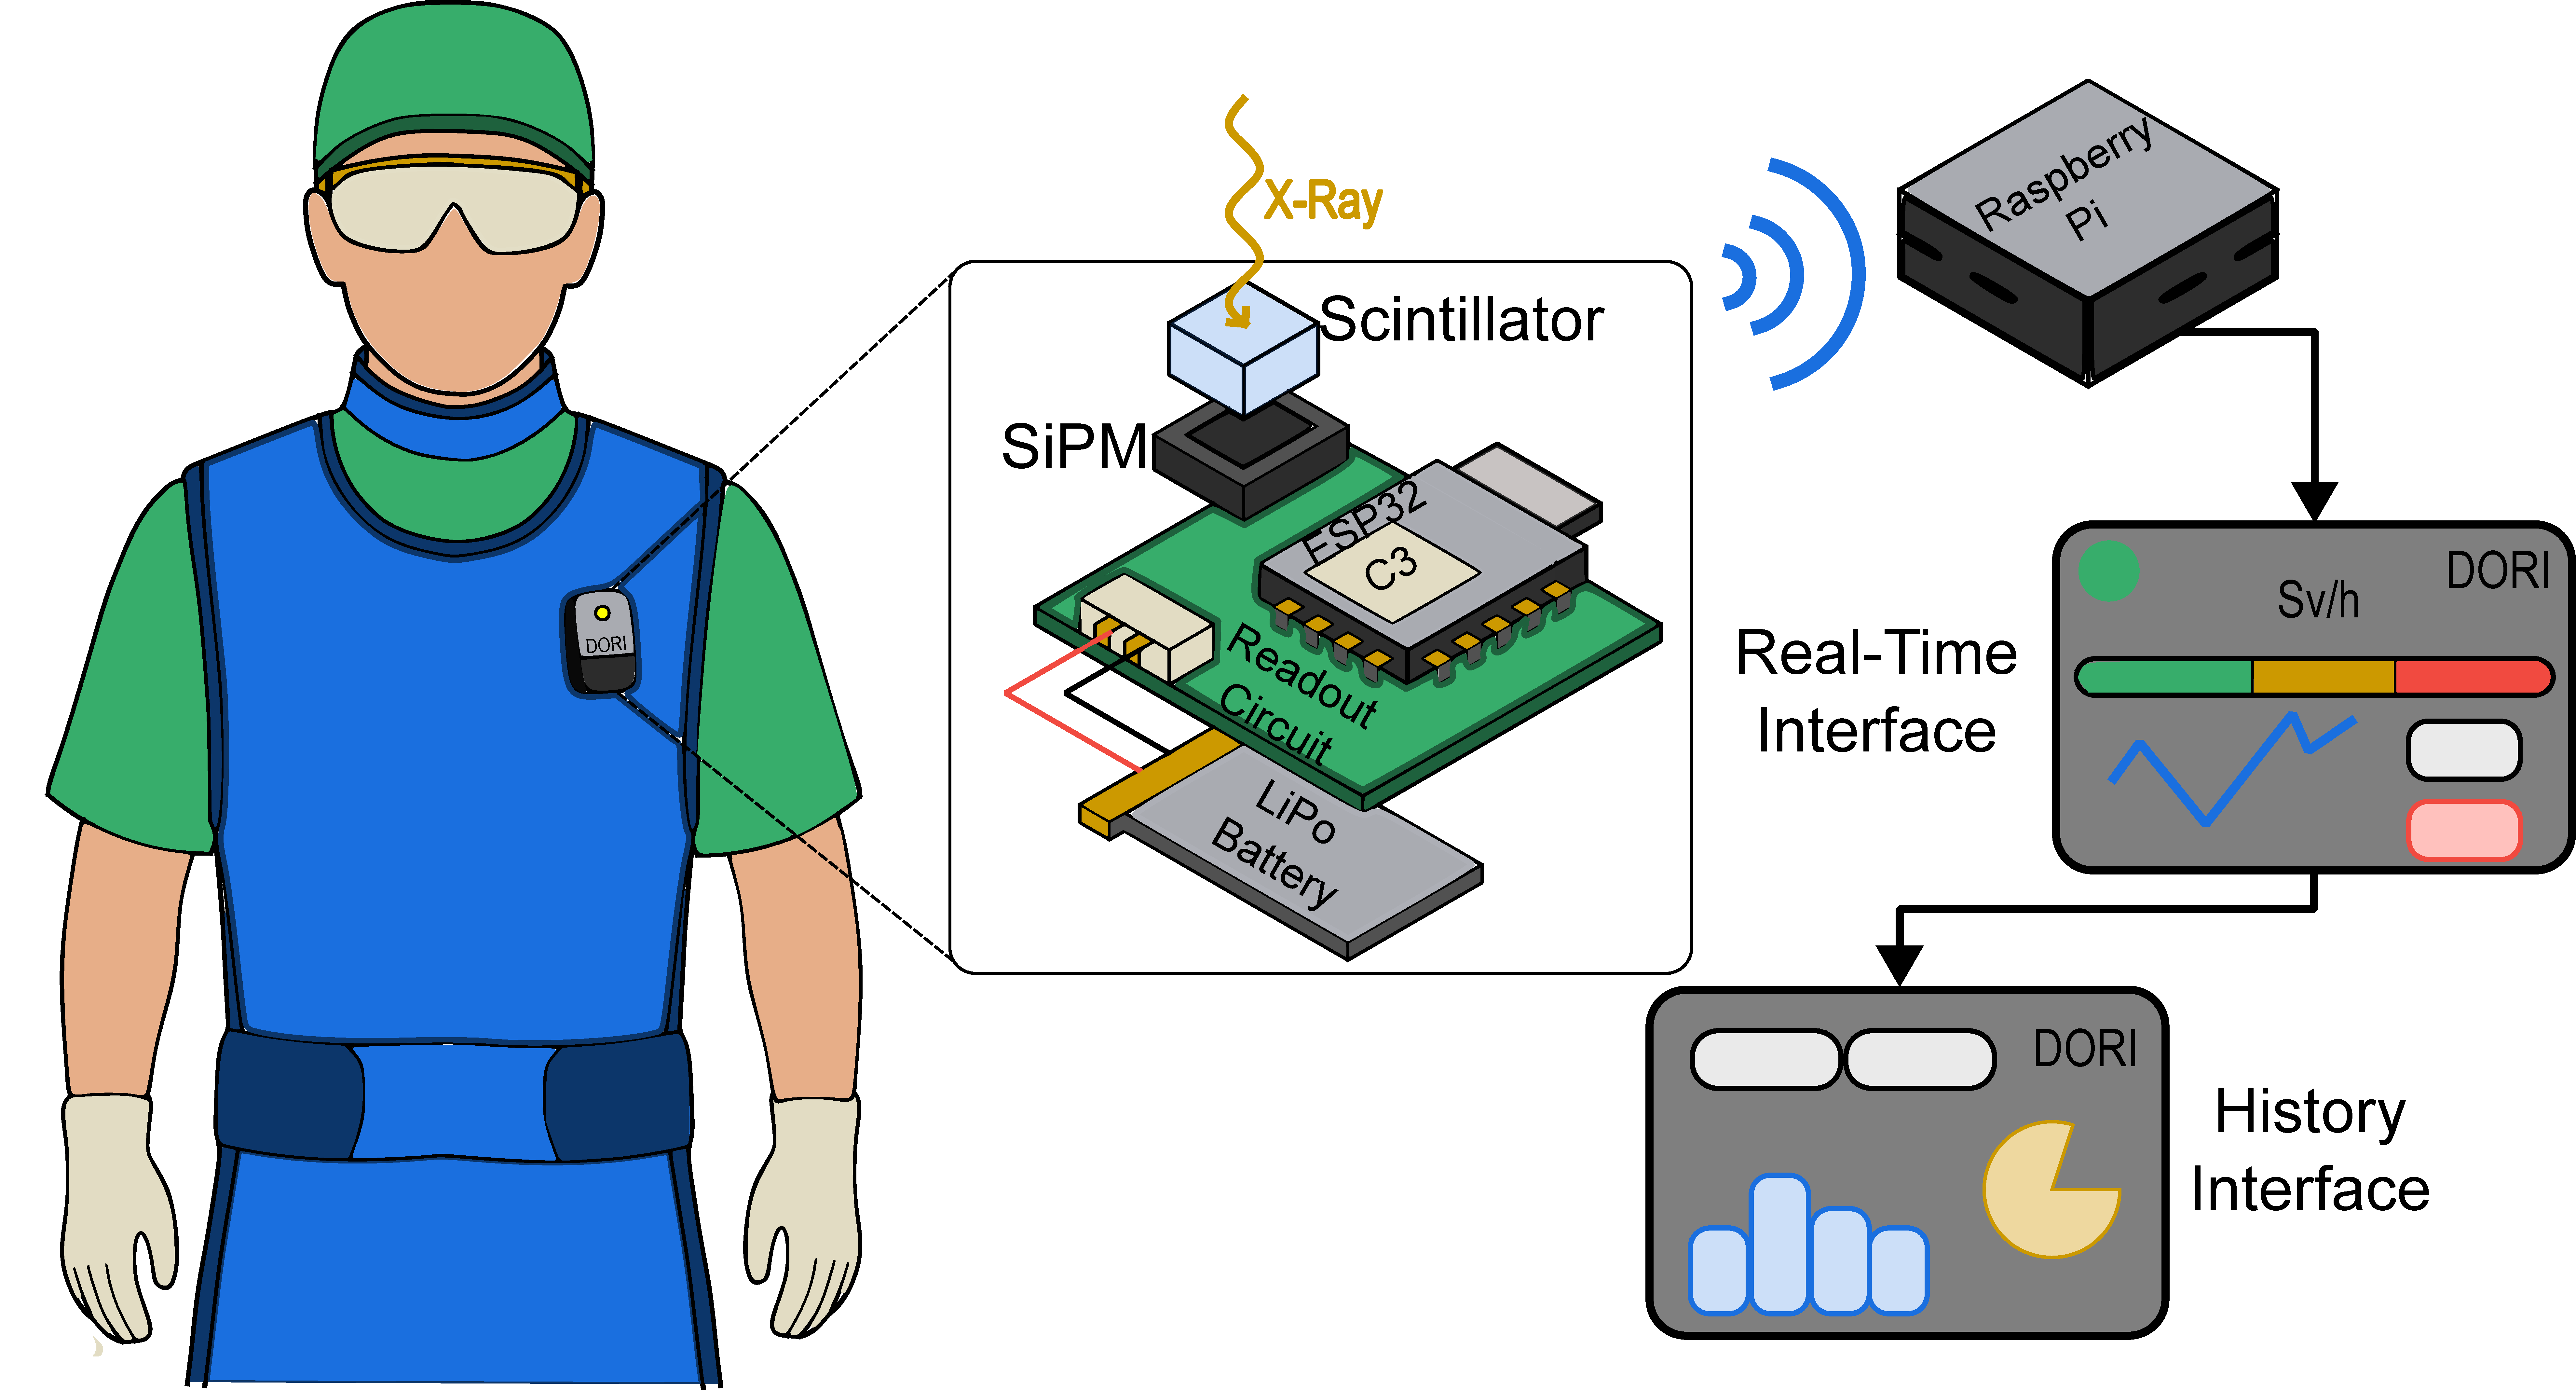
\includegraphics[width=\linewidth]{images/DORI.pdf}
  \caption[Conceptual design of DORI.]{Conceptual design of DORI. The wearable unit (exploded
view) is worn over the protective apron and comprises the scintillator,
photodetector, readout circuit, MCU and LiPo battery. Data are sent to a
Raspberry Pi, which displays the real-time and history interfaces.}
  \label{fig:DORI}
\end{figure}
DORI consists of a compact wearable unit, worn over the protective apron, which integrates the full detection, pulse processing and transmission chain. Each stage is described in detail in the following sections. In general terms, scattered radiation interacts with a scintillator, and the resulting light is converted into an electrical signal by a photodetector.
DORI operates in pulse mode, where each interaction is registered as an individual event. The corresponding pulse is conditioned by a readout board, which preserves the amplitude and thereby the energy deposited in each event. By accounting for the energy of individual interactions, rather than integrating total charge, the accuracy of the dose calculation can be improved. The target energy range is 20 to 100~keV, corresponding to the energies of the scattered field in IR (recall Table~\ref{tab:ir_parameters}).

The chain is controlled by a microcontroller unit (MCU) with wireless communication capabilities. The ESP32-C3 was selected for being compact, lightweight and low-cost. It supports 2.4~GHz Wi-Fi and Bluetooth\textsuperscript{\textregistered} Low Energy (BLE)~5~\cite{134}, the latter being the adopted communication protocol. Unlike Wi-Fi, BLE establishes a direct link with the receiver and requires no external router, reducing system complexity. In addition, BLE~5 offers extended range and increased data throughput relative to previous versions, meeting the requirements of continuous dose transmission. The unit is powered by a rechargeable lithium polymer (LiPo) battery, the AKYGA LP103040~\cite{135}, whose 1200~mAh capacity supports uninterrupted operation over extended periods. The selected Seeed Studio XIAO ESP32-C3~\cite{133} board already incorporates a charging circuit for the battery via its USB-C port. Accordingly, the front-end electronics operate at a 3.3~V logic level.

To preserve battery life, the wearable unit does not compute dose. The MCU accumulates the amplitude information of the detected events and transmits it via BLE at a one-second rate to a Raspberry Pi. Since the Raspberry Pi is permanently powered, it handles all data processing, from pulse amplitude to energy and, ultimately, to dose. A real-time interface then displays the dose rate with a complementary colour-coded scale, updated at the same one-second rate. The scale is replicated on an LED integrated in the wearable unit, with the corresponding colour level sent back to the badge via BLE. All measured data are also stored in an internal database, from which a second interface builds retrospective summaries of the recorded exposure.
\section{Scintillator}
\label{sec:scintillator}
The detection of the scattered radiation is based on a plastic scintillator (PS). PSs are organic materials that emit photons in the near ultraviolet to visible range when excited by ionising radiation. The selected scintillator is a $5 \times 5 \times 5$~mm$^3$ BC-408 cube. BC-408 consists of a polyvinyltoluene base doped with fluorophore compounds that shift the emission to a peak wavelength of 425~nm~\cite{128}.

The main advantage of PSs is their tissue equivalence. Their effective atomic number is also lower than that of the materials used in passive dosimeters or in solid-state diodes, like the RaySafe i3. The energy absorbed in the scintillator therefore approximates the dose to soft tissue without requiring further corrections~\cite{129}. However, as a drawback, the same tissue equivalence implies that, as in soft tissue, Compton scattering predominates over the photoelectric effect at the photon energies of the scattered field. From an energy calibration perspective, the acquired spectrum reduces to a Compton continuum without photopeaks, and the standard identification of $\gamma$-emitting radionuclides is not possible (recall Section~\ref{sec:Photon Interaction with Matter}). Consequently, the energy resolution of these detectors is poor. The only identifiable spectral feature is the CE, corresponding to the maximum energy transfer at a scattering angle of $\theta = 180^{\circ}$, whose energy is well known for a given source through Eq.\ref{eq:compton}. Nonetheless, owing to the poor energy resolution at the energies of interest, the CE may not coincide with the channel of maximum counts. To resolve this ambiguity, Compton coincidence techniques are employed, in which the backscattered photon from a CE event is detected in coincidence with a reference detector. However, these have primarily been demonstrated using $^{22}$Na and $^{137}$Cs, whose CEs lie outside the range relevant to this work~\cite{127}.

Such methods also assume a proportional response, meaning a light output that scales linearly with the deposited energy. However, below approximately 125~keV, the light output of PSs is non-proportional due to ionisation quenching. Slow (lower energy) electrons ionise the medium more densely, and part of the excitation is dissipated without the emission of light~\cite{130}. The Compton electrons produced in the PS in this work fall below this threshold. The pulse height of the detected events may therefore not be a linear measure of the deposited energy, and the response must instead be characterised locally, with any calibration valid only within the region where it is established.
\section{Photodetector}
To detect the scintillation light and convert it into an electrical signal, a silicon photomultiplier (SiPM) from Broadcom (AFBR-S4N66P014M~\cite{131}) was optically coupled to the scintillator. Its $6\times6$~mm\textsuperscript{2} active area matches the PS cross section, maximizing light collection. Additionally, the photon detection efficiency of the SiPM peaks at 420~nm, close to the peak emission of BC-408~\cite{131}.

A SiPM consists of a parallel array of avalanche photodiodes operated in Geiger mode. Each cell is reverse biased above its breakdown voltage, so a single absorbed photon is sufficient to trigger a self-sustaining avalanche. The photons produced by a scintillation event fire many pixels simultaneously, each of which contributes one identical pulse. The summed output current is proportional to the number of fired cells, and therefore to the energy deposited in the PS~\cite{14}. The number of available microcells (22\,428) fulfills the requirements given the photons produced per scintillation event. The SiPM has a breakdown voltage of 33~V and supports overvoltages of up to 16~V~\cite{131}.

\subsection{SiPM Power Supply}
\label{sec:sipm_power_supply}
The SiPM operating voltage was set to 37~V. Although gain increases with overvoltage, so do the dark count rate and crosstalk probability, which in excess mask the low-energy end of the spectrum. For the 20 to 100~keV range, an overvoltage of 4~V provides enough gain for these events to sit above noise levels. The bias is generated by a MAX1932 ~\cite{132} and its output is programmed through a Serial Peripheral Interface (SPI) by the MCU, which writes an eight-bit code to the internal DAC of the power supply.

A fixed 37~V output does not account for the variation of the breakdown voltage with temperature, which increases at 30~mV/$^\circ$C according to the SiPM datasheet~\cite{131}. Since gain depends on the overvoltage, a constant bias means the gain decreases as temperature rises. The same deposited energy then produces a different pulse amplitude, affecting the energy calibration and the derived dose. To compensate for this, an NTC thermistor was added to the feedback network, as recommended in the MAX1932 datasheet~\cite{132} and shown in Fig.~\ref{fig:bias}. The total resistance between the FB node and ground is~\cite{132}:
\begin{equation}
R_\text{total}(T) = R_8 + \frac{R_9\,R_T(T)}{R_9 + R_T(T)},
\label{eq:rtotal}
\end{equation}
The output voltage is therefore~\cite{132}:
\begin{equation}
V_\text{OUT} = 1.25\left(1 + \frac{R_5}{R_\text{total}(T)}\right) + \frac{R_5}{R_6}\left(1.25 - V_\text{DAC}\right),
\label{eq:vout_max}
\end{equation}
where $V_\text{DAC}$ is the DAC output voltage. The compensation condition requires the derivative of Eq.~\ref{eq:vout_max} to equal the temperature coefficient of the breakdown voltage over the operating range of 18 to 25~$^\circ$C:
\begin{equation}
\frac{dV_\text{OUT}}{dT} = \frac{1.25\,R_5}{R_\text{total}^2}\left(\frac{R_9}{R_9 + R_T}\right)^2 \frac{\beta}{T^2}\,R_T = 30~\text{mV/}^\circ\text{C}.
\label{eq:slope}
\end{equation}
Solving this condition together with Eqs.~\ref{eq:rtotal} and \ref{eq:vout_max} and the component selection equations of the datasheet~\cite{132} yields $R_5 = 91$~k$\Omega$, $R_6 = 27$~k$\Omega$, $R_8 = 2.4$~k$\Omega$, and $R_9 = 910$~$\Omega$.
\begin{figure}[H]
  \centering
  \resizebox{!}{5.2cm}{\tikzset{every picture/.style={line width=0.75pt}} %set default line width to 0.75pt        

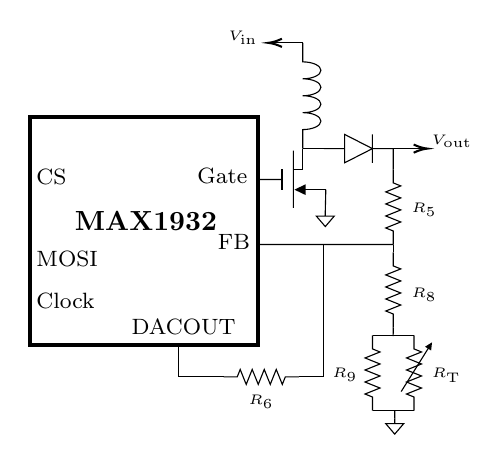
\begin{tikzpicture}[x=0.75pt,y=0.75pt,yscale=-1,xscale=1]
%uncomment if require: \path (0,300); %set diagram left start at 0, and has height of 300

%Shape: Square [id:dp45442051822513774] 
\draw  [line width=1.5]  (218.47,64.6) -- (328.47,64.6) -- (328.47,174.6) -- (218.47,174.6) -- cycle ;
%Shape: Inductor (Air Core) [id:dp8320962493713222] 
\draw   (350,29.04) -- (350,38.21) .. controls (354.83,38.21) and (358.75,40.04) .. (358.75,42.29) .. controls (358.75,44.54) and (354.83,46.37) .. (350,46.37) .. controls (354.83,46.37) and (358.75,48.19) .. (358.75,50.44) .. controls (358.75,52.69) and (354.83,54.52) .. (350,54.52) .. controls (354.83,54.52) and (358.75,56.35) .. (358.75,58.6) .. controls (358.75,60.85) and (354.83,62.67) .. (350,62.67) .. controls (354.83,62.67) and (358.75,64.5) .. (358.75,66.75) .. controls (358.75,69) and (354.83,70.83) .. (350,70.83) -- (350,80) ;
%Shape: Diode [id:dp522086168972487] 
\draw   (370.19,73.17) -- (383.57,80) -- (370.19,86.83) -- (370.19,73.17) -- cycle (360.16,80) -- (370.19,80) (383.57,73.17) -- (383.57,86.83) (383.57,80) -- (393.6,80) ;
%Shape: Resistor [id:dp8144600229276032] 
\draw   (393.61,90) -- (393.61,96.52) -- (397.22,97.97) -- (390,100.86) -- (397.22,103.76) -- (390,106.66) -- (397.22,109.55) -- (390,112.45) -- (397.22,115.35) -- (390,118.24) -- (393.61,119.69) -- (393.61,126.21) ;
%Straight Lines [id:da29049231672487486] 
\draw    (340,90) -- (340,100) ;
%Straight Lines [id:da4316288408593886] 
\draw    (361.11,99.78) -- (348.99,99.78) ;
\draw [shift={(345.99,99.78)}, rotate = 360] [fill={rgb, 255:red, 0; green, 0; blue, 0 }  ][line width=0.08]  [draw opacity=0] (5.36,-2.57) -- (0,0) -- (5.36,2.57) -- cycle    ;
%Straight Lines [id:da6953106373785519] 
\draw    (361.11,99.78) -- (360.86,110) ;
%Shape: Ground [id:dp011205472514209114] 
\draw   (356.54,112.52) -- (360.86,117.56) -- (365.17,112.52) -- (356.54,112.52) -- cycle (360.86,110) -- (360.86,112.52) ;
%Straight Lines [id:da5829290803316644] 
\draw    (350,80) -- (360.16,80) ;
%Straight Lines [id:da05768888846435982] 
\draw    (345.48,80.94) -- (345.5,108.61) ;
%Straight Lines [id:da31478243553340524] 
\draw    (350,80) -- (350,90) ;
%Straight Lines [id:da2330593515607322] 
\draw    (350,90) -- (345.79,90) ;
%Straight Lines [id:da3584287863409543] 
\draw    (328.59,94.89) -- (340.16,94.88) ;
%Shape: Resistor [id:dp4537216327878536] 
\draw   (393.61,130) -- (393.61,136.52) -- (397.22,137.97) -- (390,140.86) -- (397.22,143.76) -- (390,146.66) -- (397.22,149.55) -- (390,152.45) -- (397.22,155.35) -- (390,158.24) -- (393.61,159.69) -- (393.61,166.21) ;
%Shape: Resistor [id:dp44213159457902096] 
\draw   (383.61,170) -- (383.61,176.52) -- (387.22,177.97) -- (380,180.86) -- (387.22,183.76) -- (380,186.66) -- (387.22,189.55) -- (380,192.45) -- (387.22,195.35) -- (380,198.24) -- (383.61,199.69) -- (383.61,206.21) ;
%Shape: Resistor [id:dp5279058570816227] 
\draw   (403.61,170) -- (403.61,176.52) -- (407.22,177.97) -- (400,180.86) -- (407.22,183.76) -- (400,186.66) -- (407.22,189.55) -- (400,192.45) -- (407.22,195.35) -- (400,198.24) -- (403.61,199.69) -- (403.61,206.21) ;
%Shape: Ground [id:dp21864911769776485] 
\draw   (390,212.52) -- (394.31,217.56) -- (398.63,212.52) -- (390,212.52) -- cycle (394.31,210) -- (394.31,212.52) ;
%Shape: Resistor [id:dp5330487161197813] 
\draw   (311.9,190) -- (318.41,190) -- (319.86,186.39) -- (322.76,193.61) -- (325.65,186.39) -- (328.55,193.61) -- (331.45,186.39) -- (334.35,193.61) -- (337.24,186.39) -- (340.14,193.61) -- (341.59,190) -- (348.1,190) ;
%Straight Lines [id:da903277102568916] 
\draw    (397.43,197.05) -- (410.69,175.88) ;
\draw [shift={(412.29,173.33)}, rotate = 122.07] [fill={rgb, 255:red, 0; green, 0; blue, 0 }  ][line width=0.08]  [draw opacity=0] (3.57,-1.72) -- (0,0) -- (3.57,1.72) -- cycle    ;
%Straight Lines [id:da6627028399578476] 
\draw    (393.61,126.21) -- (393.61,130) ;
%Straight Lines [id:da19956176075595244] 
\draw    (383.61,170) -- (403.61,170) ;
%Straight Lines [id:da9867546245054489] 
\draw    (393.61,166.21) -- (393.56,170.39) ;
%Straight Lines [id:da699703638594996] 
\draw    (383.61,206.21) -- (403.61,206.21) ;
%Straight Lines [id:da6230017749012404] 
\draw    (394.3,206.05) -- (394.31,210) ;
%Straight Lines [id:da5942027422502576] 
\draw    (393.61,90) -- (393.6,80) ;
%Straight Lines [id:da7853613457386626] 
\draw    (393.61,126.21) -- (328.37,126.2) ;
%Straight Lines [id:da6727874772719629] 
\draw    (290,174.57) -- (290,190) ;
%Straight Lines [id:da9301720203284228] 
\draw    (311.9,190) -- (290,190) ;
%Straight Lines [id:da23173374113205025] 
\draw    (360,126.43) -- (360,190) ;
%Straight Lines [id:da39088728409946005] 
\draw    (348.1,190) -- (360,190) ;
%Straight Lines [id:da34090922258728096] 
\draw    (350,29.04) -- (335.39,29.04) ;
\draw [shift={(333.39,29.04)}, rotate = 360] [color={rgb, 255:red, 0; green, 0; blue, 0 }  ][line width=0.75]    (6.56,-1.97) .. controls (4.17,-0.84) and (1.99,-0.18) .. (0,0) .. controls (1.99,0.18) and (4.17,0.84) .. (6.56,1.97)   ;
%Straight Lines [id:da06307080945568311] 
\draw    (390,80) -- (408,80) ;
\draw [shift={(410,80)}, rotate = 180] [color={rgb, 255:red, 0; green, 0; blue, 0 }  ][line width=0.75]    (6.56,-1.97) .. controls (4.17,-0.84) and (1.99,-0.18) .. (0,0) .. controls (1.99,0.18) and (4.17,0.84) .. (6.56,1.97)   ;

% Text Node
\draw (298,88.22) node [anchor=north west][inner sep=0.75pt]  [font=\small] [align=left] {{\footnotesize Gate}};
% Text Node
\draw (307.9,120.17) node [anchor=north west][inner sep=0.75pt]  [font=\small] [align=left] {{\footnotesize FB}};
% Text Node
\draw (266.24,160.79) node [anchor=north west][inner sep=0.75pt]  [font=\small] [align=left] {{\footnotesize DACOUT}};
% Text Node
\draw (220.44,88.89) node [anchor=north west][inner sep=0.75pt]  [font=\small] [align=left] {{\footnotesize CS}};
% Text Node
\draw (220.44,128.33) node [anchor=north west][inner sep=0.75pt]  [font=\small] [align=left] {{\footnotesize MOSI}};
% Text Node
\draw (220.44,148.56) node [anchor=north west][inner sep=0.75pt]  [font=\small] [align=left] {{\footnotesize Clock}};
% Text Node
\draw (239,109) node [anchor=north west][inner sep=0.75pt]   [align=left] {\textbf{MAX1932}};
% Text Node
\draw (313,22) node [anchor=north west][inner sep=0.75pt]  [font=\tiny] [align=left] {$V_{\text{in}}$};
% Text Node
\draw (411,72) node [anchor=north west][inner sep=0.75pt]  [font=\tiny] [align=left] {$V_{\text{out}}$};
% Text Node
\draw (401.22,105.01) node [anchor=north west][inner sep=0.75pt]  [font=\tiny] [align=left] {$R_5$};
% Text Node
\draw (401.22,145.9) node [anchor=north west][inner sep=0.75pt]  [font=\tiny] [align=left] {$R_8$};
% Text Node
\draw (411,184.49) node [anchor=north west][inner sep=0.75pt]  [font=\tiny] [align=left] {$R_{\text{T}}$};
% Text Node
\draw (363,184.49) node [anchor=north west][inner sep=0.75pt]  [font=\tiny] [align=left] {$R_9$};
% Text Node
\draw (322.67,197.6) node [anchor=north west][inner sep=0.75pt]  [font=\tiny] [align=left] {$R_6$};

\end{tikzpicture}}
  \caption[SiPM bias supply.]{MAX1932 feedback network with the NTC thermistor $R_T$ for temperature compensation of the SiPM bias. Pin labels on the left correspond to SPI connections.}
  \label{fig:bias}
\end{figure}



\section{Front-End Electronics}
\label{sec:front_end}
The front-end electronics perform the pulse-mode readout of the SiPM response. The architecture developed for this purpose is represented by the simplified block diagram in Fig.~\ref{fig:architecture}, and includes three stages. Pulse shaping integrates and filters the SiPM current into a voltage pulse whose amplitude is proportional to the collected charge. Pulse discrimination then compares this pulse against a reference threshold, rejecting noise, and retains its peak amplitude. Pulse sampling digitises the held value through an Analog-to-Digital Converter (ADC) and transmits it to the MCU. Each stage is detailed in the following sections.

The front-end electronics were assembled on a printed circuit board (PCB), which also integrates the ESP32-C3, the MAX1932 bias supply and the SiPM described previously. The DORI-test board is shown in Fig.~\ref{fig:pcb} (a). The scintillator and the SiPM are not soldered directly on the board. Instead, the two are optically coupled and enclosed in an individual light-tight printed box, connected to the readout chain through a pin header. This arrangement allows the detector elements to be replaced without reworking the board, so that different configurations can be evaluated with the same electronics. All measurements presented in this work were performed with three sealed radioactive sources, $^{241}$Am, $^{109}$Cd and $^{57}$Co, selected because their emissions fall within the energy range of interest. Further information on their activities can be found in Appendix~A. A test box was 3D printed to align each source with the active area of the photosensitive housing, as shown in Fig.~\ref{fig:pcb} (b). The box additionally reduces the handling of the sources and allows a greater distance to be maintained during testing, contributing to a lower radiation exposure.
\begin{figure}[H]
  \centering
  \resizebox{\linewidth}{!}{

\tikzset{every picture/.style={line width=0.75pt}} %set default line width to 0.75pt        

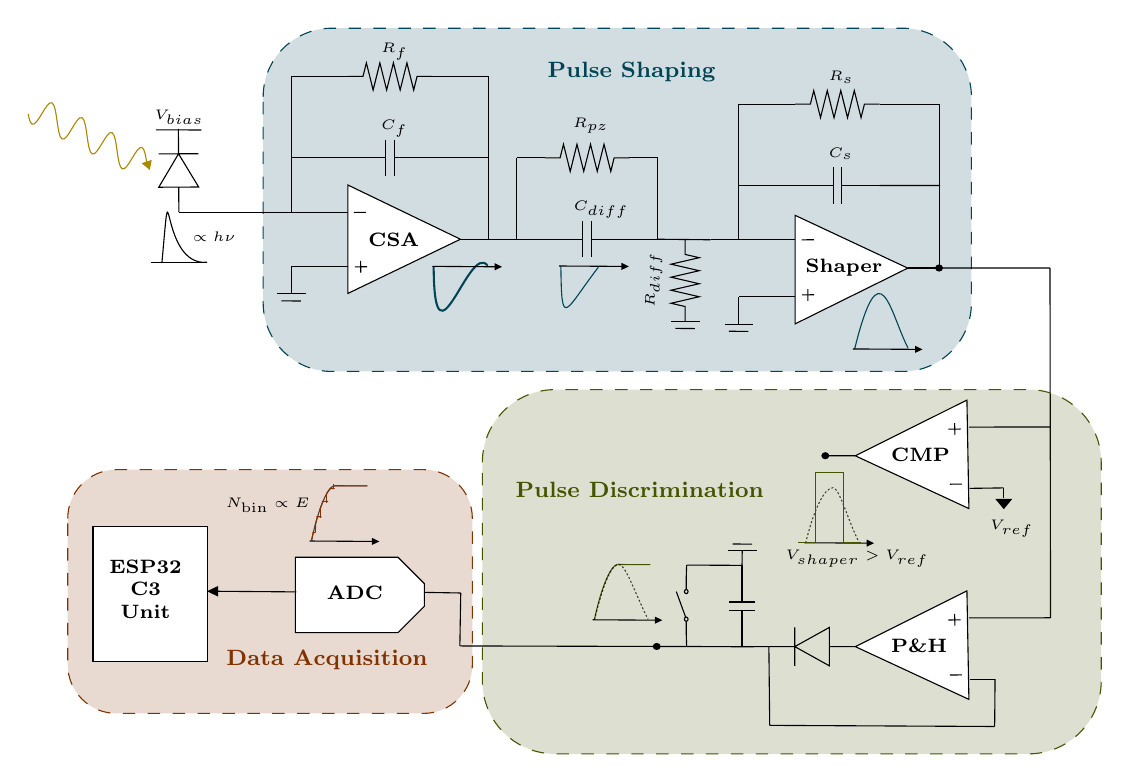
\begin{tikzpicture}[x=0.75pt,y=0.75pt,yscale=-1,xscale=1]
%uncomment if require: \path (0,390); %set diagram left start at 0, and has height of 390

%Rounded Rect [id:dp46800229916678826] 
\draw  [color={rgb, 255:red, 128; green, 51; blue, 0 }  ,draw opacity=1 ][fill={rgb, 255:red, 128; green, 51; blue, 0 }  ,fill opacity=0.18 ][dash pattern={on 4.5pt off 4.5pt}] (75.7,255.44) .. controls (75.7,242.46) and (86.22,231.95) .. (99.19,231.95) -- (247.14,231.95) .. controls (260.12,231.95) and (270.63,242.46) .. (270.63,255.44) -- (270.63,325.9) .. controls (270.63,338.88) and (260.12,349.39) .. (247.14,349.39) -- (99.19,349.39) .. controls (86.22,349.39) and (75.7,338.88) .. (75.7,325.9) -- cycle ;
%Rounded Rect [id:dp6060718292152891] 
\draw  [color={rgb, 255:red, 0; green, 68; blue, 85 }  ,draw opacity=1 ][fill={rgb, 255:red, 0; green, 68; blue, 85 }  ,fill opacity=0.18 ][dash pattern={on 4.5pt off 4.5pt}] (169.85,52.35) .. controls (169.85,34.09) and (184.66,19.28) .. (202.92,19.28) -- (478.01,19.28) .. controls (496.28,19.28) and (511.09,34.09) .. (511.09,52.35) -- (511.09,151.57) .. controls (511.09,169.84) and (496.28,184.64) .. (478.01,184.64) -- (202.92,184.64) .. controls (184.66,184.64) and (169.85,169.84) .. (169.85,151.57) -- cycle ;
%Straight Lines [id:da20418652663852965] 
\draw    (118.17,68.23) -- (140.04,68.31) ;
%Shape: Diode [id:dp9073484797643522] 
\draw   (119.56,95.88) -- (129.08,79.78) -- (138.77,95.78) -- (119.56,95.88) -- cycle (129.23,107.87) -- (129.17,95.83) (119.47,79.83) -- (138.68,79.73) (129.08,79.78) -- (129.01,67.74) ;
%Straight Lines [id:da29328469712985317] 
\draw    (129.23,107.87) -- (210.63,107.87) ;
%Shape: Triangle [id:dp7568885508488827] 
\draw  [fill={rgb, 255:red, 255; green, 255; blue, 255 }  ,fill opacity=1 ] (264.89,120.94) -- (210.63,147.08) -- (210.63,94.8) -- cycle ;
%Straight Lines [id:da4819348879555857] 
\draw    (210.63,134.01) -- (183.5,134.01) ;
%Straight Lines [id:da645749601403131] 
\draw    (183.5,147.08) -- (183.5,134.01) ;
%Straight Lines [id:da6803870332982462] 
\draw    (176.71,147.27) -- (190.28,147.27) ;
%Straight Lines [id:da005605298303441364] 
\draw    (178.65,150.63) -- (188.04,150.71) ;
%Straight Lines [id:da05308331089564988] 
\draw    (183.5,107.87) -- (183.5,81.73) ;
%Straight Lines [id:da020906030143946763] 
\draw    (183.5,42.51) -- (183.5,94.8) ;
%Shape: Resistor [id:dp7434947714198523] 
\draw   (210.63,42.51) -- (217.95,42.51) -- (219.58,35.98) -- (222.83,49.05) -- (226.09,35.98) -- (229.35,49.05) -- (232.6,35.98) -- (235.86,49.05) -- (239.11,35.98) -- (242.37,49.05) -- (244,42.51) -- (251.32,42.51) ;
%Shape: Capacitor [id:dp42145798620234975] 
\draw   (210.63,81.73) -- (228.94,81.73) (233.01,72.99) -- (233.01,90.46) (228.94,72.99) -- (228.94,90.46) (233.01,81.73) -- (251.32,81.73) ;
%Straight Lines [id:da34880193469214116] 
\draw    (210.63,42.51) -- (183.5,42.51) ;
%Straight Lines [id:da026503265572629386] 
\draw    (264.89,120.94) -- (292.02,120.94) ;
%Straight Lines [id:da9274117024294998] 
\draw    (278.45,42.51) -- (278.45,120.94) ;
%Straight Lines [id:da7747280381922488] 
\draw    (251.32,42.51) -- (278.45,42.51) ;
%Straight Lines [id:da1032408852686264] 
\draw    (183.5,81.73) -- (210.63,81.73) ;
%Straight Lines [id:da1423279487465121] 
\draw    (251.32,81.73) -- (278.45,81.73) ;
%Curve Lines [id:da7997259707368105] 
\draw [color={rgb, 255:red, 0; green, 0; blue, 0 }  ,draw opacity=1 ][fill={rgb, 255:red, 255; green, 255; blue, 255 }  ,fill opacity=1 ]   (121.09,132.03) .. controls (126.11,76.56) and (119.49,134.29) .. (142.8,132.03) ;
%Straight Lines [id:da9485003249156622] 
\draw    (115.67,132.03) -- (142.8,132.03) ;
%Curve Lines [id:da49583939836969093] 
\draw [color={rgb, 255:red, 0; green, 68; blue, 85 }  ,draw opacity=1 ]   (313.29,133.84) .. controls (313.63,164.72) and (314.85,155.96) .. (331.36,134.4) ;
%Shape: Resistor [id:dp18008683636522793] 
\draw   (305.58,81.73) -- (312.91,81.73) -- (314.54,75.19) -- (317.79,88.26) -- (321.05,75.19) -- (324.3,88.26) -- (327.56,75.19) -- (330.81,88.26) -- (334.07,75.19) -- (337.33,88.26) -- (338.95,81.73) -- (346.28,81.73) ;
%Straight Lines [id:da6245327821504196] 
\draw    (292.02,120.94) -- (292.02,81.73) ;
%Straight Lines [id:da9330542602485921] 
\draw    (292.02,81.73) -- (305.58,81.73) ;
%Straight Lines [id:da7057152830278173] 
\draw    (292.02,120.94) -- (305.58,120.94) ;
%Shape: Capacitor [id:dp8095550086511366] 
\draw   (305.58,120.94) -- (323.9,120.94) (327.97,112.21) -- (327.97,129.67) (323.9,112.21) -- (323.9,129.67) (327.97,120.94) -- (346.28,120.94) ;
%Straight Lines [id:da5386226934871385] 
\draw    (346.28,81.73) -- (359.84,81.73) ;
%Straight Lines [id:da7313083657794016] 
\draw    (346.28,120.94) -- (359.84,120.94) ;
%Straight Lines [id:da03131911441569635] 
\draw    (359.84,81.73) -- (359.84,120.94) ;
%Curve Lines [id:da7413273067238557] 
\draw [color={rgb, 255:red, 0; green, 68; blue, 85 }  ,draw opacity=1 ][line width=0.75]    (252,134.01) .. controls (252.17,187.85) and (269.17,121.74) .. (278,133.68) ;
%Shape: Triangle [id:dp6184826935280519] 
\draw  [fill={rgb, 255:red, 255; green, 255; blue, 255 }  ,fill opacity=1 ] (480.43,134.86) -- (426.17,161.72) -- (426.17,109.44) -- cycle ;
%Straight Lines [id:da31773246729249327] 
\draw    (426.17,148.65) -- (399.03,148.65) ;
%Straight Lines [id:da3550332613541024] 
\draw    (399.03,161.72) -- (399.03,148.65) ;
%Straight Lines [id:da8025351063037379] 
\draw    (392.25,161.91) -- (405.82,161.91) ;
%Straight Lines [id:da02403217066549712] 
\draw    (394.19,165.27) -- (403.58,165.35) ;
%Straight Lines [id:da16841076045424963] 
\draw    (385.47,121.2) -- (426.17,121.2) ;
%Straight Lines [id:da5746709989474186] 
\draw    (399.03,121.2) -- (399.03,95.06) ;
%Straight Lines [id:da2718623980119098] 
\draw    (399.03,55.84) -- (399.03,108.13) ;
%Shape: Resistor [id:dp29501269522921625] 
\draw   (426.17,55.84) -- (433.49,55.84) -- (435.12,49.31) -- (438.37,62.38) -- (441.63,49.31) -- (444.89,62.38) -- (448.14,49.31) -- (451.4,62.38) -- (454.65,49.31) -- (457.91,62.38) -- (459.54,55.84) -- (466.86,55.84) ;
%Shape: Capacitor [id:dp6295648569904636] 
\draw   (426.17,95.06) -- (444.48,95.06) (448.55,86.32) -- (448.55,103.79) (444.48,86.32) -- (444.48,103.79) (448.55,95.06) -- (466.86,95.06) ;
%Straight Lines [id:da39447831240426734] 
\draw    (426.17,55.84) -- (399.03,55.84) ;
%Straight Lines [id:da7401181488947025] 
\draw    (548.94,134.81) -- (549.21,303.33) ;
%Straight Lines [id:da3780881206944031] 
\draw    (466.86,55.84) -- (495.5,55.84) ;
%Straight Lines [id:da4232645895231355] 
\draw    (399.03,95.06) -- (426.17,95.06) ;
%Straight Lines [id:da4266027647624573] 
\draw    (466.86,95.06) -- (495.95,95.05) ;
%Straight Lines [id:da5672944700293289] 
\draw    (480.43,134.8) -- (495.5,134.8) ;
%Straight Lines [id:da469893720694727] 
\draw    (213.52,108.04) -- (219.36,107.98) ;
%Straight Lines [id:da9392787125105846] 
\draw    (251.32,134.01) -- (281.93,134.21) ;
\draw [shift={(284.93,134.23)}, rotate = 180.37] [fill={rgb, 255:red, 0; green, 0; blue, 0 }  ][line width=0.08]  [draw opacity=0] (3.57,-1.72) -- (0,0) -- (3.57,1.72) -- cycle    ;
%Straight Lines [id:da6932257001220354] 
\draw    (312.44,133.84) -- (343.05,134.03) ;
\draw [shift={(346.05,134.05)}, rotate = 180.37] [fill={rgb, 255:red, 0; green, 0; blue, 0 }  ][line width=0.08]  [draw opacity=0] (3.57,-1.72) -- (0,0) -- (3.57,1.72) -- cycle    ;
%Straight Lines [id:da6166140138845793] 
\draw    (214.06,134.25) -- (219.9,134.19) ;
%Shape: Boxed Line [id:dp7328235768970041] 
\draw    (216.82,131.4) -- (216.87,137.02) ;
%Straight Lines [id:da9592107478171705] 
\draw    (429.33,121.24) -- (435.17,121.18) ;
%Shape: Boxed Line [id:dp06578186279615383] 
\draw    (432.26,145) -- (432.31,150.63) ;
%Straight Lines [id:da21273186496269592] 
\draw    (429.48,147.76) -- (435.31,147.69) ;
%Shape: Resistor [id:dp07090411488435666] 
\draw   (373.14,121.2) -- (373.14,128.26) -- (379.92,129.83) -- (366.35,132.97) -- (379.92,136.1) -- (366.35,139.24) -- (379.92,142.38) -- (366.35,145.51) -- (379.92,148.65) -- (366.35,151.79) -- (373.14,153.36) -- (373.14,160.42) ;
%Straight Lines [id:da5181129573733605] 
\draw    (366.56,160.54) -- (380.13,160.54) ;
%Straight Lines [id:da36868876671547046] 
\draw    (368.5,163.9) -- (377.89,163.98) ;
%Straight Lines [id:da4086711222947753] 
\draw    (359.84,120.94) -- (385.47,121.2) ;
%Rounded Rect [id:dp3460824200505386] 
\draw  [color={rgb, 255:red, 68; green, 85; blue, 0 }  ,draw opacity=1 ][fill={rgb, 255:red, 68; green, 85; blue, 0 }  ,fill opacity=0.18 ][dash pattern={on 4.5pt off 4.5pt}] (275.46,228.49) .. controls (275.46,209.1) and (291.18,193.39) .. (310.56,193.39) -- (538.52,193.39) .. controls (557.91,193.39) and (573.62,209.1) .. (573.62,228.49) -- (573.62,333.79) .. controls (573.62,353.18) and (557.91,368.89) .. (538.52,368.89) -- (310.56,368.89) .. controls (291.18,368.89) and (275.46,353.18) .. (275.46,333.79) -- cycle ;
%Shape: Triangle [id:dp21057859356469377] 
\draw  [fill={rgb, 255:red, 255; green, 255; blue, 255 }  ,fill opacity=1 ] (455.14,225.28) -- (508.92,198.42) -- (509.87,250.71) -- cycle ;
%Straight Lines [id:da7294664906139928] 
\draw    (506.48,238.91) -- (500.65,238.97) ;
%Shape: Boxed Line [id:dp3537895946781868] 
\draw    (503.13,215.14) -- (502.98,209.52) ;
%Straight Lines [id:da9669577971099538] 
\draw    (505.86,212.39) -- (500.02,212.45) ;
%Straight Lines [id:da8006808934622864] 
\draw    (510.26,240.97) -- (526.57,240.75) ;
%Shape: Triangle [id:dp4851626389643716] 
\draw  [fill={rgb, 255:red, 0; green, 0; blue, 0 }  ,fill opacity=1 ] (526.69,250.57) -- (523.14,246.29) -- (530.24,246.29) -- cycle ;
%Straight Lines [id:da7399314250868523] 
\draw    (455.14,225.28) -- (440.69,225.25) ;
%Flowchart: Connector [id:dp3531466314065995] 
\draw  [fill={rgb, 255:red, 0; green, 0; blue, 0 }  ,fill opacity=1 ] (493.88,134.8) .. controls (493.88,134) and (494.61,133.35) .. (495.5,133.35) .. controls (496.39,133.35) and (497.11,134) .. (497.11,134.8) .. controls (497.11,135.59) and (496.39,136.24) .. (495.5,136.24) .. controls (494.61,136.24) and (493.88,135.59) .. (493.88,134.8) -- cycle ;
%Straight Lines [id:da9446115204522941] 
\draw    (509.88,211.45) -- (549.21,211.39) ;
%Curve Lines [id:da31175352604231354] 
\draw [color={rgb, 255:red, 0; green, 68; blue, 85 }  ,draw opacity=1 ]   (454.82,173.8) .. controls (467.17,123.88) and (471.61,155.96) .. (480.63,173.55) ;
%Straight Lines [id:da8734375505712497] 
\draw    (453.91,173.8) -- (484.52,174) ;
\draw [shift={(487.51,174.02)}, rotate = 180.37] [fill={rgb, 255:red, 0; green, 0; blue, 0 }  ][line width=0.08]  [draw opacity=0] (3.57,-1.72) -- (0,0) -- (3.57,1.72) -- cycle    ;
%Straight Lines [id:da6007611642847911] 
\draw    (430.57,267.17) -- (461.17,267.37) ;
\draw [shift={(464.17,267.38)}, rotate = 180.37] [fill={rgb, 255:red, 0; green, 0; blue, 0 }  ][line width=0.08]  [draw opacity=0] (3.57,-1.72) -- (0,0) -- (3.57,1.72) -- cycle    ;
%Curve Lines [id:da5409343504904985] 
\draw [color={rgb, 255:red, 0; green, 0; blue, 0 }  ,draw opacity=0.7 ] [dash pattern={on 0.75pt off 0.75pt on 0.75pt off 0.75pt}]  (431.19,267.37) .. controls (436.14,247.38) and (441.17,240.57) .. (444.39,240.68) .. controls (447.6,240.8) and (451.6,256.57) .. (457.01,267.12) ;
%Shape: Pulse Wave Form [id:dp37814170861699237] 
\draw  [color={rgb, 255:red, 68; green, 85; blue, 0 }  ,draw opacity=1 ] (427.44,267.23) -- (435.91,267.23) -- (435.91,233.36) -- (449.48,233.36) -- (449.48,267.23) -- (457.96,267.23) ;

%Straight Lines [id:da8033158731026477] 
\draw    (328.55,304.29) -- (359.16,304.48) ;
\draw [shift={(362.16,304.5)}, rotate = 180.37] [fill={rgb, 255:red, 0; green, 0; blue, 0 }  ][line width=0.08]  [draw opacity=0] (3.57,-1.72) -- (0,0) -- (3.57,1.72) -- cycle    ;
%Curve Lines [id:da8165839321439692] 
\draw [color={rgb, 255:red, 68; green, 85; blue, 0 }  ,draw opacity=1 ]   (329.46,304.29) .. controls (330.89,296.83) and (335.71,278.62) .. (340.54,277.66) ;
%Straight Lines [id:da9249993527350234] 
\draw [color={rgb, 255:red, 68; green, 85; blue, 0 }  ,draw opacity=1 ]   (340.54,277.66) -- (356.36,277.74) ;
%Curve Lines [id:da01278581006202073] 
\draw [color={rgb, 255:red, 0; green, 0; blue, 0 }  ,draw opacity=0.7 ] [dash pattern={on 0.75pt off 0.75pt on 0.75pt off 0.75pt}]  (329.46,304.29) .. controls (334.41,284.3) and (338.09,277.46) .. (341.3,277.57) .. controls (344.51,277.68) and (349.87,293.49) .. (355.27,304.04) ;
%Straight Lines [id:da36645697031500035] 
\draw    (526.57,245.78) -- (526.57,240.75) ;
%Shape: Triangle [id:dp48501946316287736] 
\draw  [fill={rgb, 255:red, 255; green, 255; blue, 255 }  ,fill opacity=1 ] (455.14,317.22) -- (508.92,290.36) -- (509.87,342.64) -- cycle ;
%Straight Lines [id:da6036906170346914] 
\draw    (506.48,330.84) -- (500.65,330.91) ;
%Shape: Boxed Line [id:dp6726482576478763] 
\draw    (503.13,307.08) -- (502.98,301.45) ;
%Straight Lines [id:da037444841152633135] 
\draw    (505.86,304.32) -- (500.02,304.39) ;
%Straight Lines [id:da5709459533271122] 
\draw    (510.26,332.91) -- (522.47,332.91) ;
%Straight Lines [id:da19356976941121384] 
\draw    (509.88,303.38) -- (549.21,303.33) ;
%Shape: Diode [id:dp614316518769653] 
\draw   (442.65,326.48) -- (425.99,317.22) -- (442.65,307.96) -- (442.65,326.48) -- cycle (455.14,317.22) -- (442.65,317.22) (425.99,326.48) -- (425.99,307.96) (425.99,317.22) -- (413.5,317.22) ;
%Straight Lines [id:da09813703953082598] 
\draw    (413.5,317.22) -- (413.9,355.16) ;
%Straight Lines [id:da849214487415646] 
\draw    (413.9,355.16) -- (522.28,355.7) ;
%Straight Lines [id:da125511136072201] 
\draw    (522.47,332.91) -- (522.28,355.7) ;
%Shape: Capacitor [id:dp7142356900456059] 
\draw   (400.56,278.07) -- (400.56,295.71) (407,299.63) -- (394.12,299.63) (407,295.71) -- (394.12,295.71) (400.56,299.63) -- (400.56,317.28) ;
%Shape: Simple Switch [id:dp5297728261178234] 
\draw   (373.67,310.11) -- (373.67,305) (373.67,289.68) -- (373.67,284.57) (373.37,302.96) -- (368.9,290.7) (373.67,291.72) .. controls (373.18,291.72) and (372.78,291.26) .. (372.78,290.7) .. controls (372.78,290.14) and (373.18,289.68) .. (373.67,289.68) .. controls (374.17,289.68) and (374.57,290.14) .. (374.57,290.7) .. controls (374.57,291.26) and (374.17,291.72) .. (373.67,291.72) -- cycle (373.67,305) .. controls (373.18,305) and (372.78,304.54) .. (372.78,303.98) .. controls (372.78,303.42) and (373.18,302.96) .. (373.67,302.96) .. controls (374.17,302.96) and (374.57,303.42) .. (374.57,303.98) .. controls (374.57,304.54) and (374.17,305) .. (373.67,305) -- cycle ;
%Straight Lines [id:da9962880185364887] 
\draw    (400.56,278.07) -- (373.87,277.93) ;
%Straight Lines [id:da4168400592441782] 
\draw    (400.56,317.28) -- (373.87,317.15) ;
%Straight Lines [id:da6629627230865746] 
\draw    (373.87,277.93) -- (373.67,284.57) ;
%Straight Lines [id:da6227335867281195] 
\draw    (373.67,310.11) -- (373.87,317.15) ;
%Straight Lines [id:da9440197749138511] 
\draw    (400.56,317.28) -- (413.5,317.22) ;
%Straight Lines [id:da5574398837436616] 
\draw    (373.87,317.15) -- (359.47,317.14) ;
%Flowchart: Connector [id:dp28586564232252365] 
\draw  [fill={rgb, 255:red, 0; green, 0; blue, 0 }  ,fill opacity=1 ] (439.08,225.25) .. controls (439.08,224.45) and (439.8,223.81) .. (440.69,223.81) .. controls (441.58,223.81) and (442.3,224.45) .. (442.3,225.25) .. controls (442.3,226.05) and (441.58,226.69) .. (440.69,226.69) .. controls (439.8,226.69) and (439.08,226.05) .. (439.08,225.25) -- cycle ;
%Flowchart: Connector [id:dp5135507227534388] 
\draw  [fill={rgb, 255:red, 0; green, 0; blue, 0 }  ,fill opacity=1 ] (357.86,317.14) .. controls (357.86,316.35) and (358.58,315.7) .. (359.47,315.7) .. controls (360.36,315.7) and (361.08,316.35) .. (361.08,317.14) .. controls (361.08,317.94) and (360.36,318.58) .. (359.47,318.58) .. controls (358.58,318.58) and (357.86,317.94) .. (357.86,317.14) -- cycle ;
%Shape: Wave [id:dp059927494842615836] 
\draw  [color={rgb, 255:red, 170; green, 136; blue, 0 }  ,draw opacity=1 ] (56.66,60.65) .. controls (57.1,63.11) and (57.63,65.03) .. (58.51,65.46) .. controls (59.82,66.11) and (61.52,63.3) .. (63.3,60.33) .. controls (65.08,57.37) and (66.78,54.56) .. (68.09,55.21) .. controls (69.4,55.86) and (69.96,59.8) .. (70.54,63.93) .. controls (71.12,68.06) and (71.67,72) .. (72.98,72.65) .. controls (74.29,73.3) and (75.99,70.48) .. (77.77,67.52) .. controls (79.55,64.56) and (81.25,61.75) .. (82.56,62.4) .. controls (83.87,63.05) and (84.43,66.98) .. (85,71.12) .. controls (85.58,75.25) and (86.14,79.19) .. (87.45,79.84) .. controls (88.76,80.49) and (90.46,77.67) .. (92.24,74.71) .. controls (94.02,71.75) and (95.72,68.94) .. (97.03,69.59) .. controls (98.34,70.24) and (98.89,74.17) .. (99.47,78.31) .. controls (100.05,82.44) and (100.61,86.38) .. (101.92,87.03) .. controls (103.23,87.68) and (104.93,84.86) .. (106.71,81.9) .. controls (108.49,78.94) and (110.19,76.12) .. (111.5,76.77) .. controls (112.71,77.37) and (113.27,80.78) .. (113.81,84.55) ;
%Shape: Triangle [id:dp3108622029974263] 
\draw  [color={rgb, 255:red, 170; green, 136; blue, 0 }  ,draw opacity=1 ][fill={rgb, 255:red, 170; green, 136; blue, 0 }  ,fill opacity=1 ] (115.05,87.07) -- (111.86,84.44) -- (115.81,83.09) -- cycle ;
%Straight Lines [id:da5842921754561695] 
\draw    (400.56,278.07) -- (400.66,271.23) ;
%Straight Lines [id:da97191101904161] 
\draw    (396,267.77) -- (400.92,267.81) -- (405.39,267.84) ;
%Straight Lines [id:da8202699426795026] 
\draw    (393.99,271.03) -- (395.72,271.03) -- (407.56,271.03) ;
%Snip Same Side Corner Rect [id:dp24267720786095204] 
\draw  [fill={rgb, 255:red, 255; green, 255; blue, 255 }  ,fill opacity=1 ] (234.8,274.15) -- (247.52,286.87) -- (247.52,297.77) -- (234.8,310.49) -- (185.39,310.49) -- (185.39,310.49) -- (185.39,274.15) -- (185.39,274.15) -- cycle ;
%Shape: Rectangle [id:dp4960716974860516] 
\draw  [fill={rgb, 255:red, 255; green, 255; blue, 255 }  ,fill opacity=1 ] (87.86,259.38) -- (142.94,259.38) -- (142.94,324.22) -- (87.86,324.22) -- cycle ;
%Straight Lines [id:da5259235282088736] 
\draw    (264.62,316.89) -- (359.47,317.14) ;
%Straight Lines [id:da04918323557857496] 
\draw    (247.85,291.09) -- (265.04,291.38) ;
%Straight Lines [id:da700345769463564] 
\draw    (265.04,291.38) -- (264.62,316.89) ;
%Straight Lines [id:da44513384727711636] 
\draw    (192.21,266.34) -- (222.82,266.54) ;
\draw [shift={(225.82,266.56)}, rotate = 180.37] [fill={rgb, 255:red, 0; green, 0; blue, 0 }  ][line width=0.08]  [draw opacity=0] (3.57,-1.72) -- (0,0) -- (3.57,1.72) -- cycle    ;
%Curve Lines [id:da06577028557977793] 
\draw [color={rgb, 255:red, 0; green, 0; blue, 0 }  ,draw opacity=0.7 ]   (193.12,266.34) .. controls (194.55,258.88) and (199.36,240.67) .. (204.19,239.71) ;
%Straight Lines [id:da0572237289311508] 
\draw [color={rgb, 255:red, 0; green, 0; blue, 0 }  ,draw opacity=0.7 ]   (204.19,239.71) -- (220.01,239.8) ;
%Curve Lines [id:da3804043288541633] 
\draw [color={rgb, 255:red, 128; green, 51; blue, 0 }  ,draw opacity=1 ] [dash pattern={on 3pt off 3pt on 3pt off 3pt}]  (193.12,266.34) .. controls (194.55,258.88) and (199.36,240.67) .. (204.19,239.71) ;
%Straight Lines [id:da5333998307295363] 
\draw [color={rgb, 255:red, 128; green, 51; blue, 0 }  ,draw opacity=1 ]   (193.63,262.21) -- (195,262.32) ;
%Straight Lines [id:da40393427405433224] 
\draw [color={rgb, 255:red, 128; green, 51; blue, 0 }  ,draw opacity=1 ]   (195,262.32) -- (195.08,258.23) ;
%Straight Lines [id:da3824884565346163] 
\draw [color={rgb, 255:red, 128; green, 51; blue, 0 }  ,draw opacity=1 ]   (202.04,241.08) -- (204.32,241.09) ;
%Straight Lines [id:da8760345808356574] 
\draw [color={rgb, 255:red, 128; green, 51; blue, 0 }  ,draw opacity=1 ]   (203.75,241.36) -- (203.75,239.04) ;

%Straight Lines [id:da012864593156911797] 
\draw [color={rgb, 255:red, 128; green, 51; blue, 0 }  ,draw opacity=1 ]   (195.47,254.61) -- (197.96,254.68) ;
%Straight Lines [id:da7563678124476333] 
\draw [color={rgb, 255:red, 128; green, 51; blue, 0 }  ,draw opacity=1 ]   (197.4,255.23) -- (197.4,250.54) ;
%Straight Lines [id:da5333243365793827] 
\draw [color={rgb, 255:red, 128; green, 51; blue, 0 }  ,draw opacity=1 ]   (198.85,247.27) -- (198.18,247.22) -- (201.13,247.28) ;
%Straight Lines [id:da6175946543817453] 
\draw [color={rgb, 255:red, 128; green, 51; blue, 0 }  ,draw opacity=1 ]   (200.56,247.82) -- (200.56,247.22) -- (200.56,243.14) ;
%Straight Lines [id:da3521344691026579] 
\draw [color={rgb, 255:red, 128; green, 51; blue, 0 }  ,draw opacity=1 ]   (204.19,239.71) -- (220.01,239.8) ;
%Straight Lines [id:da18368526561352316] 
\draw    (185.87,290.85) -- (145.8,290.54) ;
\draw [shift={(142.8,290.52)}, rotate = 0.43] [fill={rgb, 255:red, 0; green, 0; blue, 0 }  ][line width=0.08]  [draw opacity=0] (5.36,-2.57) -- (0,0) -- (5.36,2.57) -- cycle    ;
%Straight Lines [id:da56033182920969] 
\draw    (495.5,55.84) -- (495.5,133.35) ;
%Straight Lines [id:da784442544187718] 
\draw    (495.5,134.8) -- (548.94,134.81) ;

% Text Node
\draw (225.47,25.29) node [anchor=north west][inner sep=0.75pt]  [font=\tiny] [align=left] {$R_{f}$};
% Text Node
\draw (225.47,62.28) node [anchor=north west][inner sep=0.75pt]  [font=\tiny] [align=left] {$C_{f}$};
% Text Node
\draw (116.3,57.49) node [anchor=north west][inner sep=0.75pt]  [font=\tiny] [align=left] {$V_{bias}$};
% Text Node
\draw (134.54,116.18) node [anchor=north west][inner sep=0.75pt] [font=\tiny] {\(\propto h\nu\)};
% Text Node
\draw (317.75,61.5) node [anchor=north west][inner sep=0.75pt]  [font=\tiny] [align=left] {$R_{pz}$};
% Text Node
\draw (318.11,101.49) node [anchor=north west][inner sep=0.75pt]  [font=\tiny] [align=left] {$C_{diff}$};
% Text Node
\draw (441.01,38.62) node [anchor=north west][inner sep=0.75pt]  [font=\tiny] [align=left] {$R_{s}$};
% Text Node
\draw (441.01,75.61) node [anchor=north west][inner sep=0.75pt]  [font=\tiny] [align=left] {$C_{s}$};
% Text Node
\draw (219.33,116.63) node [anchor=north west][inner sep=0.75pt]  [font=\scriptsize] [align=left] {{\scriptsize \textbf{CSA}}};
% Text Node
\draw (430,129) node [anchor=north west][inner sep=0.75pt]  [font=\scriptsize] [align=left] {{\scriptsize \textbf{Shaper}}};
% Text Node
\draw (305.69,34.53) node [anchor=north west][inner sep=0.75pt]   [align=left] {\textbf{{\footnotesize \textcolor[rgb]{0,0.27,0.33}{Pulse Shaping}}}};
% Text Node
\draw (352.68,155.01) node [anchor=north west][inner sep=0.75pt]  [font=\tiny,rotate=-270] [align=left] {$R_{diff}$};
% Text Node
\draw (518.87,255.11) node [anchor=north west][inner sep=0.75pt]  [font=\tiny] [align=left] {$V_{ref}$};
% Text Node
\draw (471.18,220.38) node [anchor=north west][inner sep=0.75pt]  [font=\scriptsize] [align=left] {{\scriptsize \textbf{CMP}}};
% Text Node
\draw (420.26,269.33) node [anchor=north west][inner sep=0.75pt]   [align=left] {{\tiny $V_{shaper} > V_{ref}$}};
% Text Node
\draw (471.18,312.13) node [anchor=north west][inner sep=0.75pt]  [font=\scriptsize] [align=left] {{\scriptsize \textbf{P\&H}}};
% Text Node
\draw (290.23,236.5) node [anchor=north west][inner sep=0.75pt]   [align=left] {\textbf{{\footnotesize \textcolor[rgb]{0.27,0.33,0}{Pulse Discrimination}}}};
% Text Node
\draw (199.34,286.87) node [anchor=north west][inner sep=0.75pt]  [font=\scriptsize] [align=left] {{\scriptsize \textbf{ADC}}};
% Text Node
\draw (94.49,274.48) node [anchor=north west][inner sep=0.75pt] [font=\scriptsize] [align=center] {
\textbf{ESP32}\\
\textbf{C3}\\
\textbf{Unit}
};
% Text Node
\draw (150.9,317.64) node [anchor=north west][inner sep=0.75pt]   [align=left] {\textbf{{\footnotesize \textcolor[rgb]{0.5,0.2,0}{Data Acquisition}}}};
% Text Node
\draw (150.67,244.28) node [anchor=north west][inner sep=0.75pt]  [font=\tiny] [align=left] {$N_{\text{bin}} \propto E$};

\end{tikzpicture}


}
  \caption[Architecture of the DORI system.]{Architecture of the DORI system.}
  \label{fig:architecture}
\end{figure}

\begin{figure}[H]
  \centering
  \begin{minipage}[c]{0.52\linewidth}
    \centering
    \subfloat[]{\label{fig:pcb_test}%
      \resizebox{\linewidth}{!}{\begin{tikzpicture}[x=1pt,y=1pt,
    every node/.style={font=\footnotesize},
    ah/.style={draw opacity=0,line width=0.08,fill opacity=1},
    lbl/.style={fill=white,align=center,inner sep=2.5pt,line width=0.6pt},
    dim/.style={fill=white,align=center,inner sep=2pt,draw=none,font=\scriptsize},
    reg/.style={line width=1.2pt}]

% ---- Photograph -------------------------------------------------------
\node [anchor=south west,inner sep=0] at (0,0)
  {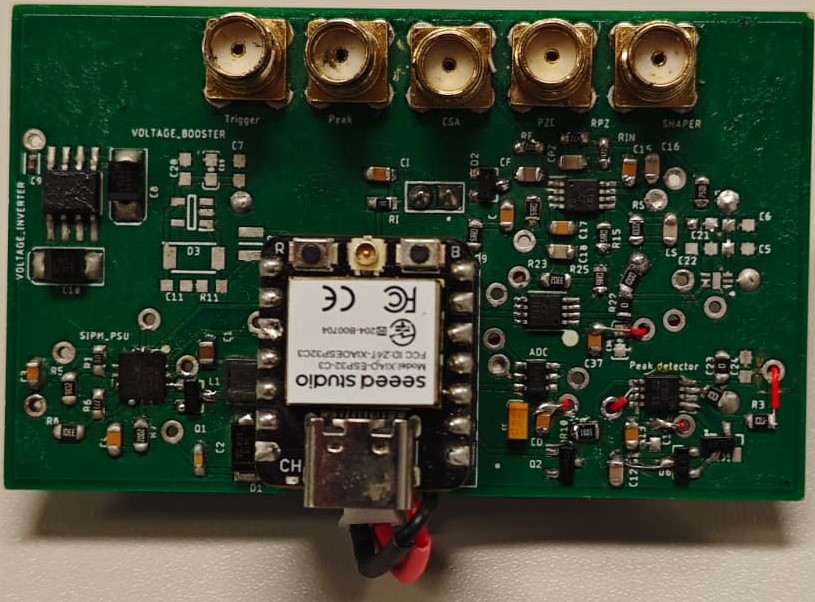
\includegraphics[width=186pt,height=127pt]{images/pcb_teste.jpg}};

% ---- Region outlines ---------------------------------------------------
\draw [reg,color={rgb, 255:red, 241; green, 74; blue, 64 }]
      (2.55,24.84) rectangle (52.93,59.98);                 % SiPM power supply
\draw [reg,color={rgb, 255:red, 26; green, 111; blue, 223 }]
      (116.09,72.67) rectangle (166.47,101.07);             % pulse shaping
\draw [reg,color={rgb, 255:red, 204; green, 153; blue, 0 }]
      (113.63,34.27) rectangle (129.67,53.47);              % ADC
\draw [reg,color={rgb, 255:red, 55; green, 173; blue, 107 }]
      (113.51,63.72) .. controls (118.22,73.60) and (139.09,68.88) .. (153.45,57.88)
   .. controls (167.81,46.87) and (177.68,49.12) .. (178.35,43.95)
   .. controls (179.03,38.79) and (182.39,38.56) .. (172.97,30.48)
   .. controls (163.55,22.40) and (163.98,22.18) .. (151.65,21.95)
   .. controls (139.33,21.72) and (126.97,19.26) .. (126.86,25.54)
   .. controls (126.74,31.83) and (140.14,43.95) .. (136.62,50.01)
   .. controls (133.10,56.08) and (108.80,53.84) .. (113.51,63.72) -- cycle ;

% ---- Labels over the board (no arrows) --------------------------------
\node [lbl,draw=none,font=\scriptsize,anchor=center] at (83.33,54.66) {MCU};
\node [lbl,draw={rgb, 255:red, 204; green, 153; blue, 0 },
       font=\scriptsize,anchor=center] at (114.30,27.04) {ADC};
\node [lbl,draw={rgb, 255:red, 241; green, 74; blue, 64 },anchor=center]
      at (27.90,13.25) {SiPM\\Power Supply};
\node [lbl,draw={rgb, 255:red, 55; green, 173; blue, 107 },anchor=center]
      at (163,13.25) {Pulse\\Discrimination};

% ---- Pulse shaping (right of the board) -------------------------------
\node [lbl,draw={rgb, 255:red, 26; green, 111; blue, 223 },anchor=west]
      at (165,86.90) {Pulse\\Shaping};



% ---- Signal test points (only arrow in the figure) --------------------
\node [lbl,draw={rgb, 255:red, 81; green, 81; blue, 81 },anchor=center]
      at (27.60,88) {Signal\\Test Points};
\draw [color={rgb, 255:red, 81; green, 81; blue, 81 },line width=1.1pt] (50,99) -- (50,108);
\draw [shift={(50,116)},rotate=270,ah,fill={rgb, 255:red, 81; green, 81; blue, 81 }]
      (7.85,-3.78) -- (0,0) -- (7.85,3.78) -- cycle ;

% ---- Width dimension (7 cm) --------------------------------------------
\draw [line width=1.1pt,black] (3.56,134) -- (184.42,134);
\draw [shift={(3.56,134)},rotate=0,ah,fill=black]
      (7.85,-3.78) -- (0,0) -- (7.85,3.78) -- cycle ;
\draw [shift={(184.42,134)},rotate=180,ah,fill=black]
      (7.85,-3.78) -- (0,0) -- (7.85,3.78) -- cycle ;
\node [dim,anchor=center] at (94,134) {7~cm};

% ---- Height dimension (4.3 cm) -----------------------------------------
\draw [line width=1.1pt,black] (-8,23.50) -- (-8,125.65);
\draw [shift={(-8,23.50)},rotate=90,ah,fill=black]
      (7.85,-3.78) -- (0,0) -- (7.85,3.78) -- cycle ;
\draw [shift={(-8,125.65)},rotate=270,ah,fill=black]
      (7.85,-3.78) -- (0,0) -- (7.85,3.78) -- cycle ;
\node [dim,anchor=center,rotate=90] at (-8,74.60) {4.3~cm};

\end{tikzpicture}}}
  \end{minipage}%
  \hfill%
  \begin{minipage}[c]{0.48\linewidth}
    \centering
    \subfloat[]{\label{fig:dori_case}%
      \resizebox{\linewidth}{!}{\begin{tikzpicture}[x=1pt,y=1pt,
    every node/.style={font=\footnotesize},
    ah/.style={draw opacity=0,line width=0.08,fill opacity=1},
    lbl/.style={fill=white,fill opacity=0.88,text opacity=1,
                align=center,inner sep=2.5pt,line width=0.6pt},
    dim/.style={fill=white,align=center,inner sep=2pt,draw=none,font=\scriptsize}]

% ---- Photograph -------------------------------------------------------
\node [anchor=south west,inner sep=0] at (0,0)
  {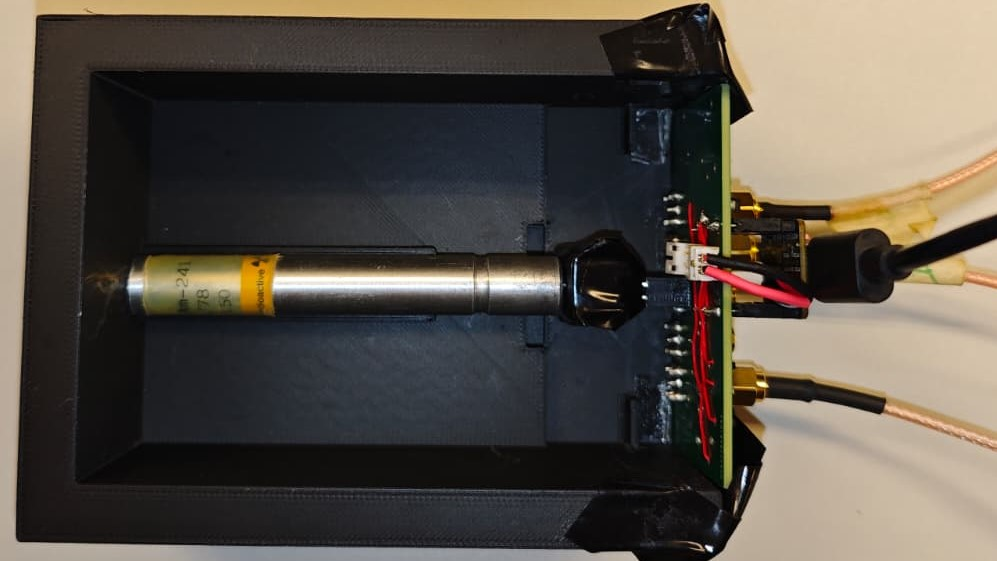
\includegraphics[width=200pt,height=127.1pt]{images/dori_case.jpg}};

% ---- 12 cm dimension (above the image, black) -------------------------
\draw [line width=1.1pt,black] (8.8,134) -- (144.4,134);
\draw [shift={(8.8,134)},rotate=0,ah,fill=black]
      (7.85,-3.78) -- (0,0) -- (7.85,3.78) -- cycle ;
\draw [shift={(144.4,134)},rotate=180,ah,fill=black]
      (7.85,-3.78) -- (0,0) -- (7.85,3.78) -- cycle ;
\node [dim,anchor=center] at (76.6,134) {12~cm};

% ---- Source holder -----------------------------------------------------
\node [anchor=south,align=center,
       text={rgb, 255:red, 204; green, 153; blue, 0 }] at (78,90) {Source Holder};
\draw [color={rgb, 255:red, 204; green, 153; blue, 0 },line width=1.1pt] (62,88) -- (58.15,79.2);
\draw [shift={(55,72)},rotate=66.4,ah,fill={rgb, 255:red, 204; green, 153; blue, 0 }]
      (7.85,-3.78) -- (0,0) -- (7.85,3.78) -- cycle ;
\draw [color={rgb, 255:red, 204; green, 153; blue, 0 },line width=1.1pt] (94,88) -- (100.4,80.5);
\draw [shift={(105.5,74.5)},rotate=130.4,ah,fill={rgb, 255:red, 204; green, 153; blue, 0 }]
      (7.85,-3.78) -- (0,0) -- (7.85,3.78) -- cycle ;

% ---- SiPM + scintillator ----------------------------------------------
\node [lbl,draw={rgb, 255:red, 26; green, 111; blue, 223 },anchor=north east]
      (sipm) at (196,112) {SiPM\\+\\Scintillator};
\draw [color={rgb, 255:red, 26; green, 111; blue, 223 },line width=1.1pt]
      (sipm.west) -| (118.1,77.4);
\draw [shift={(118.1,69.5)},rotate=90,ah,fill={rgb, 255:red, 26; green, 111; blue, 223 }]
      (7.85,-3.78) -- (0,0) -- (7.85,3.78) -- cycle ;

% ---- PCB ---------------------------------------------------------------
\node [lbl,draw={rgb, 255:red, 55; green, 173; blue, 107 },anchor=east]
      (pcb) at (196,49.9) {PCB};
\draw [color={rgb, 255:red, 55; green, 173; blue, 107 },line width=1.1pt]
      (pcb.west) -- (155.4,49.9);
\draw [shift={(147.5,49.9)},rotate=0,ah,fill={rgb, 255:red, 55; green, 173; blue, 107 }]
      (7.85,-3.78) -- (0,0) -- (7.85,3.78) -- cycle ;

% ---- 3D printed test box ----------------------------------------------
\node [lbl,draw={rgb, 255:red, 81; green, 81; blue, 81 },anchor=south east]
      (box) at (196,4) {3D Printed\\Test Box};
\draw [color={rgb, 255:red, 81; green, 81; blue, 81 },line width=1.1pt]
      (box.west) -- (131,15);
\draw [shift={(123,15)},rotate=0,ah,fill=black,
       fill={rgb, 255:red, 81; green, 81; blue, 81 }]
      (7.85,-3.78) -- (0,0) -- (7.85,3.78) -- cycle ;

\end{tikzpicture}}}
  \end{minipage}
  \caption[DORI-test board.]{%
    DORI-test board.
    \textbf{(a)} PCB with the main functional blocks identified, together with the signal test points used for characterisation;
    \textbf{(b)} assembled prototype inside the 3D printed test box, showing the sealed source holder aligned with the scintillator and SiPM.
  }
  \label{fig:pcb}
\end{figure}
\subsection{Pulse Shaping}
The current pulse produced by the SiPM delivers a quantity of charge, $Q$, that must be converted into a measurable voltage signal in the preamplifier~\cite{105}:
\begin{equation}
    Q = \int I(t)\, dt, \quad \text{unit: } [\mathrm{C}]
    \label{eq:charge}
\end{equation}

To achieve this, a Charge-Sensitive Amplifier (CSA) was implemented. The CSA is widely used as a preamplifier since the rise time of the output pulse depends only on the charge collection time in the detector, independent of both the detector and the preamplifier input capacitances~\cite{14}. It is an inverting integrator configuration designed around a low-noise operational amplifier, such as the LT6203~\cite{LT6202_LT6203_LT6204}, that was chosen accordingly. The feedback loop is closed by a capacitor $C_f$ in parallel with a resistor $R_f$~\cite{106,14}.

In this circuit, the current flows through $C_f$, allowing it to store charge and producing an output voltage proportional to $Q$. $R_f$ acts as a reset mechanism, providing a discharge path for $C_f$, in order for new pulses to be detected. The resulting output voltage can be written as~\cite{104,105}:
\begin{equation}
    V_{\text{out}} = -\frac{Q}{C_f}\, e^{-t/\tau_f}, \quad \text{unit: } [\mathrm{V}]
    \label{eq:vout}
\end{equation}

\noindent where $\tau_f = R_f C_f$ is the discharge time constant. For total
charge integration, this constant must be longer than the duration of the SiPM current pulse.

The charge gain of the CSA, $G$,  depends exclusively on $C_f$ and is therefore~\cite{106}:
\begin{equation}
    G = \frac{V_{\text{out}}}{Q} = -\frac{1}{C_f}, \quad \text{unit: } [\mathrm{V/C}]
    \label{eq:gain}
\end{equation}

To preserve the pulse amplitude, which carries the energy information of the detected events, additional signal conditioning stages were implemented. Given the high event count rate expected in IR, a Semi-Gaussian shaper was adopted in order to prevent baseline drift and relax the timing demands of the following stages. It consists of a CR differentiator followed by $n$ RC integrator stages. Increasing $n$ produces a more symmetric output pulse, which returns to baseline faster but introduces a longer peaking time~\cite{14}. For this work, a simple CR-RC ($n=1$) network was implemented, with equal differentiation and integration time constants.

The finite decay time constant of the CSA causes an undershoot at the shaper output~\cite{107}. If the signal has not recovered before the next event arrives, the subsequent pulse is superimposed on this undershoot, reducing its measured amplitude. To mitigate this effect, a Pole-Zero Cancellation (PZC) configuration was implemented. $C_{\text{diff}}$ and $R_{\text{diff}}$ form the CR differentiation network. A resistor $R_{\text{pz}}$, placed in parallel with $C_{\text{diff}}$, introduces a zero that compensates the pole produced by the CSA. Proper cancellation occurs when the following condition is satisfied~\cite{108,14,110}:
\begin{equation}
    R_{\text{pz}}\, C_{\text{diff}} = R_f\, C_f
    \label{eq:pzc}
\end{equation}

 The RC stage was implemented as an inverting low-pass filter, similar to the CSA configuration, with a feedback capacitor $C_s$ in parallel with a resistor $R_s$. As in the CSA, the gain depends on the feedback capacitor, so the value of $C_s$ controls the gain of the stage. The value of $R_s$ is then chosen so that $R_s C_s$ equals the common time constant fixed by the previous stages.

The gain of the front-end electronics was set empirically. As mentioned in Section~\ref{sec:sipm_power_supply}, the SiPM bias was fixed to keep the dark count rate at a low amplitude without masking the low-energy end of the spectrum. The gain must be high enough that real pulses are resolved above this level. It must also be low enough that the full energy range of interest, up to 100~keV, remains below saturation. The gain therefore places the spectrum in the lower portion of the available 3.3 V amplitude range.
Within this portion, enough channels must remain available to sample these energies. Following Knoll~\cite{14}, a spectral feature is adequately sampled when its full width at half maximum (FWHM) spans at least five channels. Of the reference sources available for this work, $^{241}$Am is the only one that produces a resolvable photopeak in BC-408, at
59.5~keV. The reported energy resolution of BC-408 at this energy is 30 to 50\%~\cite{119,126,127}. The narrowest case, 30\%, corresponds to a FWHM of 17.9~keV and sets the more demanding limit. Five channels across this FWHM give a channel width of 3.6~keV, and therefore a minimum of 28 channels up to 100~keV. This is a lower bound on the channel count, below which the photopeak is undersampled and energy information is lost. However, it is worth noting that such a small number of channels would be impractical for spectral characterisation, and therefore for energy calibration.

The $^{241}$Am source was nevertheless used to guide the gain. The pulses generated by the source were observed directly on the oscilloscope, and the gain was adjusted so that they did not saturate the OpAmps. It was set to remain within an amplitude range that the ADC samples with a reasonable number of channels, leaving room for the higher energies up to 100~keV. Ultimately, the gain was chosen to give finer binning while still satisfying the condition imposed by the most limiting factor, the resolution of BC-408. The resulting component values of the pulse shaping chain are listed in Table~\ref{tab:frontend}.

\vspace{1em}
\refstepcounter{table}
\label{tab:frontend}
\noindent\textbf{Table~\thetable.} Component values of the pulse shaping chain.
\addcontentsline{lot}{table}{\protect\numberline{\thetable}Component values of the pulse shaping chain.}
\vspace{0.1em}
\begin{table}[H]
  \centering
  \setlength{\tabcolsep}{12pt}
  \renewcommand{\arraystretch}{1.5}
  \begin{tabular}{c c c c c c}
    \toprule
    \multicolumn{2}{c}{\textbf{CSA}} &
    \multicolumn{2}{c}{\textbf{PZC}} &
    \multicolumn{2}{c}{\textbf{Shaper}} \\
    \cmidrule(lr){1-2}\cmidrule(lr){3-4}\cmidrule(lr){5-6}
    \textbf{Parameter} & \textbf{Value} &
    \textbf{Parameter} & \textbf{Value} &
    \textbf{Parameter} & \textbf{Value} \\
    \midrule
    \multirow{3}{*}{\shortstack{$R_f$ \\[2.2em] $C_f$}} &
    \multirow{3}{*}{\shortstack{4.7 k$\Omega$ \\[2.2em] 100 pF}} &
    $R_{\text{diff}}$ & 4.7 k$\Omega$ &
    \multirow{3}{*}{\shortstack{$R_s$ \\[2.2em] $C_s$}} &
    \multirow{3}{*}{\shortstack{10 k$\Omega$ \\[2.2em] 47 pF}} \\
    & & $R_{\text{pz}}$ & 4.7 k$\Omega$ & & \\
    & & $C_{\text{pz}}$ & 100 pF & & \\
    \midrule
    $\tau$ & 470 ns & & 470 ns & & 470 ns \\
    \bottomrule
  \end{tabular}
\end{table}

\subsubsection{Transient Response}

The transient response of the shaping chain to a single $^{241}$Am event is shown in Fig.~\ref{fig:shaping_chain}. The associated time metrics, extracted over the full set of acquired waveforms, are summarised in Table~\ref{tab:shaping}.

The integration at the CSA produces a negative pulse, since the charge is collected onto $C_f$ in an inverting configuration, and this polarity is preserved through the differentiating network. The inverting topology adopted for the last integrating stage restores a positive output at the shaper, as required by the single-positive-supply operation of the subsequent stages. A residual undershoot is nevertheless observed at every stage, originating from the CSA. Its relative magnitude is not increased along the chain, which would be the case in the absence of $R_{pz}$. The gain at the final stage was decreased, so that events of this energy are sampled towards the lower end of the available bins, as discussed. The main effect of the shaping is the redistribution of the signal in time. The semi-Gaussian output is broader and the time taken to reach the maximum is increased from $147 \pm 28$~ns at the CSA output to $387 \pm 50$~ns at the shaper, even though the latter has a lower amplitude. The interval over which the signal remains within 90\% of its maximum is doubled, from $208 \pm 167$~ns to $400 \pm 154$~ns. These effects are intended, since the amplitude is retained through comparator logic, and a maximum that is both delayed and sustained reduces the timing demands imposed on both the hardware and firmware. Within a broad range of amplitudes, the total shaping time is consistent across events, as it is set by the time constants selected for this network. At the shaper output it is $1.96 \pm 0.09$~$\mu$s, and this is the pulse the subsequent stages discriminate and sample.

\begin{figure}[H]
  \centering
  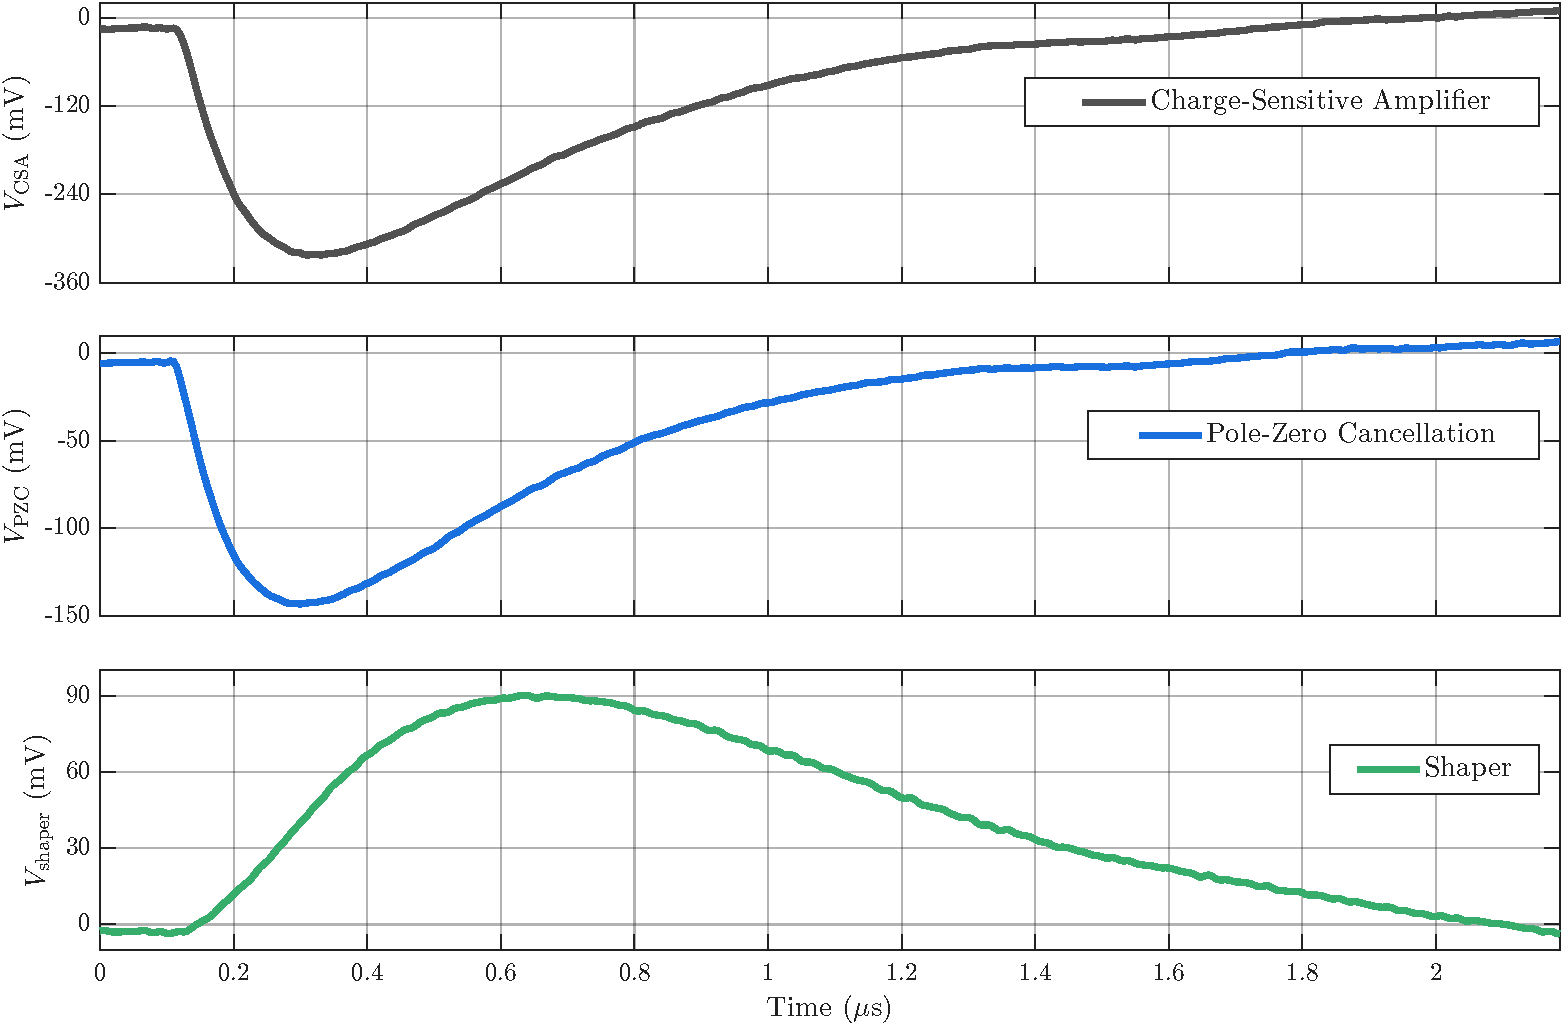
\includegraphics[width=\linewidth]{images/shaping_chain_trace00001.pdf}
  \caption[Transient response of the pulse shaping chain.]{Transient response of the CSA (grey), PZC (blue) and shaper (green) to a single $^{241}$Am event.}
  \label{fig:shaping_chain}
\end{figure}

\vspace{1em}

\refstepcounter{table}
\label{tab:shaping}
\noindent\textbf{Table~\thetable.} Timing metrics of the pulse shaping chain at each stage.
\addcontentsline{lot}{table}{\protect\numberline{\thetable}Timing metrics of the pulse shaping chain at each stage.}

\vspace{0.1em}

\begin{table}[H]
  \centering
  \setlength{\tabcolsep}{16pt}
  \renewcommand{\arraystretch}{1.65}
  \begin{tabular}{l c c c}
    \toprule
     & \textbf{CSA} & \textbf{PZC} & \textbf{Shaper} \\
    \midrule
    Amplitude range (mV)            & 191--861        & 87--430         & 61--407         \\
    Peaking time (ns)               & $147 \pm 28$    & $135 \pm 25$    & $387 \pm 50$    \\
    Width at 90\% of peak (ns)      & $208 \pm 167$   & $192 \pm 141$   & $400 \pm 154$   \\
    Total shaping time ($\mu$s)     & $1.42 \pm 0.09$ & $1.26 \pm 0.07$ & $1.96 \pm 0.09$ \\
    \bottomrule
  \end{tabular}
\end{table}


\subsection{Pulse Discrimination}
\label{sec:pulse_discrimination}

Pulse discrimination distinguishes real X-ray events from electronic noise and retains the amplitude of those accepted for digitisation. As mentioned above, it operates on a comparator logic. The LT1711~\cite{LT1711_LT1712} was selected for this application, a fast comparator operated in a non-inverting configuration. As shown in Fig.~\ref{fig:architecture}, the signal from the shaper is applied to the non-inverting input, while a fixed reference voltage, $V_{ref}$, is applied to the inverting input. The reference is derived from the 3.3 V supply rail through a resistive divider:

\begin{equation}
V_{ref} = \frac{R_2}{R_1 + R_2} \cdot 3.3, \text{ unit: [V]}
\label{eq:vref}
\end{equation}

\noindent where $R_1$ is the resistor connecting the node to the supply, and $R_2$ the resistor between the divider node and ground. The threshold was set to 10 mV. This value was established from the comparator input acquired under dark count conditions of the SiPM. The amplitudes of these events lie predominantly below 10 mV. The condition is satisfied by $R_1 = 33$ k$\Omega$ and $R_2 = 100$ $\Omega$.

A dedicated pin of the ESP32-C3 is connected to the logic output of the comparator and configured as an interrupt. Whenever the input exceeds $V_{ref}$, the comparator output switches to the logic high level. The pin is monitored continuously by dedicated hardware within the MCU, so the transition is registered as soon as it occurs. Detection initiates the readout loop, and the interrupt is detached for its duration, so that no further triggers are accepted while the event is being processed. It is reattached once the loop has terminated.

Simultaneously, the shaper output is fed to a Peak-and-Hold (P\&H) circuit. A P\&H captures the maximum of the input signal and sustains it after the pulse has decayed, extending the interval over which the peak amplitude remains available. The analogue conversion can then be performed more accurately. Given the small amplitude of the events, a configuration based on a precision rectifier is required. The adopted circuit is shown in Fig.~\ref{fig:peak_and_hold}. Two feedback paths are available to OA1. The outer path includes $D_2$ and runs from $C_H$ through the buffer OA2 and the resistor $R$ to the inverting input. The local path runs directly from the output of OA1 through $D_1$ to the same node. The two diodes are oppositely oriented, so only one path is closed at any instant, and the transition between them is determined by the position of the output of OA1 relative to the inverting input~\cite{Franco2015}.

With $C_H$ discharged and the shaped pulse rising, OA1 drives its output upwards. The anode of $D_2$ rises above its cathode, which is held at the capacitor voltage, so the diode becomes forward biased and conducts. Charge flows into $C_H$ and the capacitor voltage rises with the input. That voltage is read by OA2, and is returned through $R$ to the inverting input of OA1. Both amplifiers are implemented with the OPA354~\cite{OPA354}, whose input draws negligible current, so the stored charge cannot be drained by OA2. The amplifier therefore compares the shaped pulse against the stored voltage and continues to drive its output until the two coincide. $D_1$ is consequently reverse biased and its path is closed. This is the track mode, which is maintained until the pulse begins to decay~\cite{Franco2015}.

Once the maximum has passed, OA1 drives its output downwards. $D_2$ becomes reverse biased and the track loop is broken. At the same instant, the output of OA1 falls below the inverting input, $D_1$ becomes forward biased and establishes the local feedback path. Without this branch the amplifier would be left without feedback and driven into saturation against the negative supply, and recovery at the arrival of the following event would be governed by the slew rate. With $D_2$ reverse biased, the stored charge has no drain path through it. The remaining connections to the node are the input of OA2 and the reset path, which is held open throughout the interval. The peak value is therefore retained. This is the hold mode. The value of $C_H = 470$~pF, reflects a compromise between the two modes. A larger capacitance reduces droop during hold, but would take longer for OA1 to charge it, and higher pulses would not be held~\cite{Franco2015,Horowitz2015}.
\begin{figure}[H]
  \centering
  \tikzset{every picture/.style={line width=0.75pt}}

\begin{tikzpicture}[
    x=1.5pt, y=1.5pt, yscale=-1, xscale=1,
    every node/.style={font=\normalsize, inner sep=1pt}
]

%==================== Feedback resistor R (top rail) ====================
\draw    (200,40) -- (261.9,40) ;
\draw    (261.9,40) -- (268.41,40) -- (269.86,36.39) -- (272.76,43.61) -- (275.65,36.39) -- (278.55,43.61) -- (281.45,36.39) -- (284.35,43.61) -- (287.24,36.39) -- (290.14,43.61) -- (291.59,40) -- (298.1,40) ;
\draw    (298.1,40) -- (390,40) ;

%==================== OA_1 ====================
\draw    (210,76) -- (250,100) -- (210,124) -- cycle ;
\draw    (200,90) -- (210,90) ;
\draw    (210,110) -- (192,110) ;
\draw [shift={(190,110)}, rotate=0] [line width=0.75]
       (6.56,-1.97) .. controls (4.17,-0.84) and (1.99,-0.18) .. (0,0) .. controls (1.99,0.18) and (4.17,0.84) .. (6.56,1.97) ;
\draw    (200,40) -- (200,90) ;

%==================== D_1 (feedback diode) ====================
\draw    (200,60) -- (260,60) ;
\draw    (260,60) -- (260,73.31) ;
\draw    (266.83,73.31) -- (260,86.69) -- (253.17,73.31) -- cycle ;
\draw    (253.17,86.69) -- (266.83,86.69) ;
\draw    (260,86.69) -- (260,100) ;

%==================== D_2 (output diode) ====================
\draw    (250,100) -- (273.31,100) ;
\draw    (273.31,93.17) -- (286.69,100) -- (273.31,106.83) -- cycle ;
\draw    (286.69,93.17) -- (286.69,106.83) ;
\draw    (286.69,100) -- (340,100) ;

%==================== Hold capacitor C_h ====================
\draw    (304.5,100) -- (304.5,117) ;
\draw    (300,117) -- (309,117) ;
\draw    (300,121) -- (309,121) ;
\draw    (304.5,121) -- (304.5,140) ;
\draw    (300.19,140) -- (304.5,145) -- (308.81,140) -- cycle ;

%==================== Discharge resistor R_h ====================
\draw    (330,100) -- (330,106.74) -- (333.61,108.19) -- (326.39,111.08) -- (333.61,113.98) -- (326.39,116.88) -- (333.61,119.77) -- (326.39,122.67) -- (333.61,125.57) -- (326.39,128.46) -- (330,129.91) -- (330,144) ;

%==================== Reset MOSFET ====================
\draw    (336,141) -- (336,147) ;
\draw    (336,149) -- (336,155) ;
\draw    (336,157) -- (336,163) ;
\draw    (342,140) -- (342,164) ;
\draw    (342,152) -- (355,152) ;
\draw [shift={(357,152)}, rotate=180] [line width=0.75]
       (6.56,-1.97) .. controls (4.17,-0.84) and (1.99,-0.18) .. (0,0) .. controls (1.99,0.18) and (4.17,0.84) .. (6.56,1.97) ;
\draw    (330,144) -- (336,144) ;
\draw    (336,160) -- (330,160) ;
\draw    (330,152) -- (330,166) ;
\draw    (330,152) -- (334,152) ;
\draw [shift={(336,152)}, rotate=180] [fill={rgb, 255:red, 0; green, 0; blue, 0}, fill opacity=1] [line width=0.08] [draw opacity=0]
       (3.57,-1.72) -- (0,0) -- (3.57,1.72) -- cycle ;
\draw    (325.69,166) -- (330,171) -- (334.31,166) -- cycle ;

%==================== OA_2 ====================
\draw    (340,66) -- (380,90) -- (340,114) -- cycle ;
\draw    (330,40) -- (330,80) ;
\draw    (330,80) -- (340,80) ;
\draw    (380,90) -- (408,90) ;
\draw [shift={(410,90)}, rotate=180] [line width=0.75]
       (6.56,-1.97) .. controls (4.17,-0.84) and (1.99,-0.18) .. (0,0) .. controls (1.99,0.18) and (4.17,0.84) .. (6.56,1.97) ;
\draw    (390,40) -- (390,90) ;

%==================== Junction dots ====================
\fill (200,60)    circle (0.8) ;
\fill (260,100)   circle (0.8) ;
\fill (304.5,100) circle (0.8) ;
\fill (330,100)   circle (0.8) ;
\fill (330,40)    circle (0.8) ;
\fill (330,160)   circle (0.8) ;
\fill (390,90)    circle (0.8) ;

%==================== Labels ====================
% terminals
\draw (186,110) node [anchor=east] {V$_{\mathrm{Shaper}}$};
\draw (414,90)  node [anchor=west] {V$_{\mathrm{Peak}}$};
\draw (361,152) node [anchor=west] {Reset};

% op-amps
\draw (218,100) node [anchor=west] {OA$_{1}$};
\draw (213,90)  node [anchor=west] {$-$};
\draw (213,110) node [anchor=west] {$+$};
\draw (348,90)  node [anchor=west] {OA$_{2}$};
\draw (343,80)  node [anchor=west] {$-$};
\draw (343,100) node [anchor=west] {$+$};

% passives
\draw (280,35)  node [anchor=south] {R};
\draw (250,80)  node [anchor=east]  {D$_{1}$};
\draw (280,90)  node [anchor=south] {D$_{2}$};
\draw (298,119) node [anchor=east]  {C$_{\mathrm{h}}$};
\draw (336,119) node [anchor=west]  {R$_{\mathrm{h}}$};

\end{tikzpicture}
  \caption[Peak-and-Hold circuit.]{Peak-and-Hold circuit based on a precision rectifier. The outer feedback path of OA1 is shown at the top through $R$, while the local path closes through $D_1$.} 
  \label{fig:peak_and_hold}
\end{figure}

With no reset path, the capacitor would only ever accumulate charge. Once a maximum has been stored, a subsequent event of lower amplitude cannot forward bias $D_2$. The output would therefore converge to the largest amplitude ever received rather than to the amplitude of each individual event. A discharge path is therefore required, and it must be opened and closed under control so that $C_H$ is emptied between events. This function is performed by an N-channel MOSFET placed in series with $R_{H}=7.5$~k$\Omega$ across the capacitor, driven by a logic level from the MCU. When held low, the path between drain and source is open and the stored charge is retained. At the 3.3 V level the channel is established and the capacitor discharges through $R_H$ with a time constant $\tau = R_H C_H$. The gate is therefore held low by default, so that the circuit is always ready to capture the maximum of the signal. Detection of a valid pulse raises the interrupt described above, after which a delay of 2~$\mu$s is imposed to allow the held value to stabilise before the sampling logic is applied. The gate is then driven high for an interval longer than $\tau$, sufficient for $C_H$ to discharge, and returned low~\cite{Franco2015}.

\subsubsection{Transient Response}

The output of the pulse discrimination chain to a single $^{241}$Am event is shown in Fig.~\ref{fig:pulse_discrimination}. The trigger level was taken as the intersection between the shaper output and the comparator transition. It is measured at 9.3~mV, in agreement with the nominal threshold of approximately 10~mV. Upon reaching the maximum, the P\&H circuit retains the amplitude of the event, although a droop of the held value is present throughout the hold interval. The decay is more pronounced over the first two microseconds after the peak, which justifies the pre-sampling delay mentioned above. The residual droop over the rest of the hold is attributed to leakage through the capacitor, the diode and/or the reset path~\cite{Franco2015,Horowitz2015}.

No sampling logic was implemented for these measurements. Nevertheless, a latency is present in the transition of the transistor logical state. The hold interval is therefore extended beyond the value imposed by the firmware, which contributes directly to the dead time of the detector. Once the reset path is closed, the discharge of the storage capacitor is governed by the time constant imposed by $R_h$ and $C_h$. It was observed, however, that the output does not return to ground, settling instead at a residual baseline of approximately 50~mV. The discharge also continues after the gate has returned to the low logical state, at which point the capacitor should retain its stored voltage. This is consistent with the transition latency described above. It was first considered whether $R_h$ was too high for the discharge to complete within the time the gate sits at 3.3~V. To assess this, $R_h$ was changed to 1~k$\Omega$. Although the discharge was completed in a shorter interval, as expected, the output would settles at the same residual baseline. This behaviour could be justified with the single-supply configuration of the OpAmps. With the negative rail of OA1 connected directly to ground, the amplifier cannot reproduce the negative baseline of the shaper output. Once the reset path is open, and the input at OA1 remains negative, the current needed to supply this load may cause an output swing. This output swing would be the floor at which $C_h$ can be minimally charged. Therefore, no event below 50~mV can be sampled, as it cannot be tracked. It is a limitation of the current front-end electronics, and it reduces the dynamic range available at the lower end of the energies of interest. Ultimately, $R_h$ was kept at 7.5~k$\Omega$. Without sampling logic, the mean dead time is measured as 13~$\pm$~1~$\mu$s, taken as the interval over which the P\&H output remains at hold until it discharges to the residual baseline.

\begin{figure}[H]
  \centering
  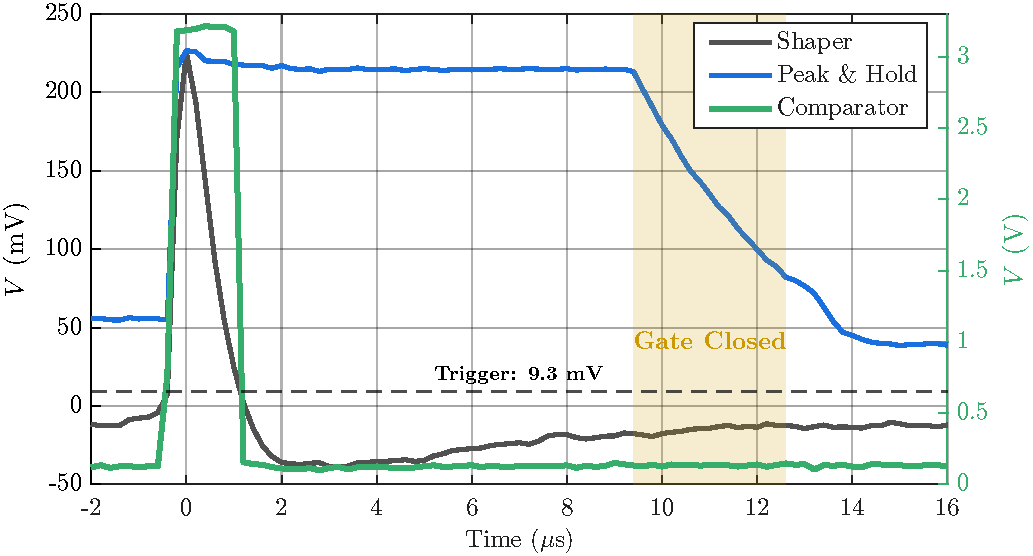
\includegraphics[width=\linewidth]{images/7.5k_notitle.pdf}
  \caption[Transient response of the pulse discrimination chain.]{Transient response of the shaper (grey), comparator (green) and P\&H (blue) stages to a single $^{241}$Am event. The yellow region marks the interval during which the reset transistor is driven HIGH, allowing the hold capacitor to discharge.}
  \label{fig:pulse_discrimination}
\end{figure}

\subsection{Pulse Sampling}
\label{sec:pulse_sampling}
Pulse sampling digitises the held signal through an ADC. The converter maps the input range onto $2^n$ discrete levels, where $n$ is its resolution in bits. Each amplitude is sampled and quantized to a corresponding digital bin. Since the conversion occupies the acquisition
chain, the introduction of a sampling stage is expected to increase the dead time of DORI. Two converters were therefore evaluated, the ADC internal to the ESP32-C3 and an external ADS7883~\cite{ADS7883}, both of 12-bit resolution. The measured dead times are presented in Table~\ref{tab:dead_time}.

\vspace{1em}
\refstepcounter{table}
\label{tab:dead_time}
\noindent \textbf{Table \thetable.} Dead time of the acquisition chain for each sampling
condition. Values are the mean of multiple $^{241}$Am events with the corresponding standard
deviation.
\vspace{0.1em}
\begin{center}
\setlength{\tabcolsep}{22pt}
\renewcommand{\arraystretch}{1.3}
\begin{tabular}{ccc}
\hline
\textbf{Sampling Condition} & \textbf{Dead Time ($\mu$s)} & \textbf{Sampling Protocol} \\
\hline
\textit{N/A} & 13.2 $\pm$ 0.9 & \textit{N/A} \\
Internal MCU ADC & 59.2 $\pm$ 1.5 & Analog Read \\
External ADC & 17.8 $\pm$ 0.4 & SPI \\
\hline
\end{tabular}
\end{center}
\vspace{1em}

From the perspective of power consumption and component complexity, the internal converter would be preferable. However, relative to the dead time measured without a sampling stage, the internal converter adds a delay ten times higher than the external one. The internal ADC is accessed through the \texttt{analogRead} routine, and limited by its own execution time, making it unsuitable for this application. On the other hand, the ADS7883 is read over SPI at 20~MHz, a dedicated high-speed protocol, and consequentely increasing the dead time by only 4.6~$\mu$s. The external converter was therefore adopted, as it allows a higher count rate to be achieved. The digitised values are subsequently rebinned to a 10-bit range in order to reduce the volume of data transmitted by the communication protocol. Over the 3.3~V input range, the resulting 1024 channels correspond to a channel width of 3.2~mV, which sets the smallest amplitude difference that can be resolved. With a dead time of 17.8~$\pm$~0.4~$\mu$s, the maximum count rate of DORI is $(56~\pm~1)\times10^{3}$~counts per second.


\section{Validation of the Front-End Electronics}
\label{sec:frontend-validation}
Prior to energy calibration of the PS, the readout electronics were validated using a $5 \times 5 \times 10$~mm CsI(Tl) crystal. The linearity of DORI can be tested by relating pulses of known energy to the channels in which they are stored. To identify an incident radionuclide emitting $\gamma$-rays, that is, to obtain the known energy pulse, photoelectric absorption must be favoured. An inorganic scintillator is appropriate for this validation owing to its higher density and effective atomic number, which favour photoelectric absorption in the energy range of interest. A linear channel-to-energy mapping is expected, and any significant deviation would be attributable to the front-end electronics~\cite{14}. This validation therefore indicates whether the front-end electronics introduce any non-linearity, such as the amplitude droop in the P\&H or its residual baseline. Should either prove amplitude-dependent, it would require characterisation or correction.

The hardware gain was adjusted to accommodate the higher light output of CsI(Tl), and spectra were acquired over 10-minute intervals using the three radioactive sources described previously. The resulting pulse height spectra are shown in Fig.~\ref{fig:validation_electronics} (a). The background was subtracted, and channels 18 and below were excluded, as its elevated count rate would otherwise dominate the vertical scale. Given the ADC step, channel 18 corresponds to a voltage of approximately 58~mV, which lies near the residual baseline of the P\&H stage. It can therefore be concluded that any event below this level is assigned to this bin, owing to the return of the hold capacitor to that charge. This does not compromise the validation, since all expected spectral features are resolved for each source, including the low energy 14.4~keV $\gamma$-ray emission of $^{57}$Co. The consequence is the masking of lower energies, and the implication for the PS calibration is that the energy range proposed must lie above this threshold.
\begin{figure}[H]
  \centering
  \subfloat[]{\label{fig:spectra}%
    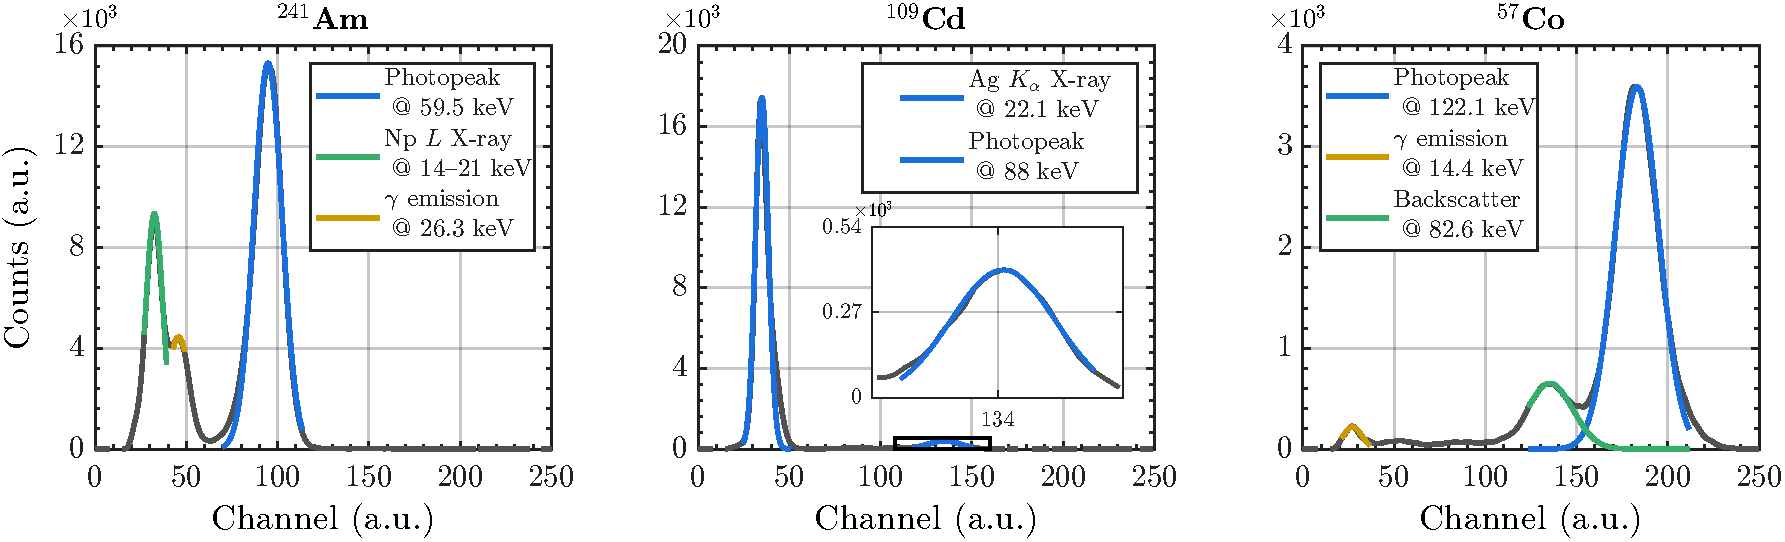
\includegraphics[width=\linewidth]{images/spectra.pdf}}\\[1ex]
  \subfloat[]{\label{fig:calib}%
    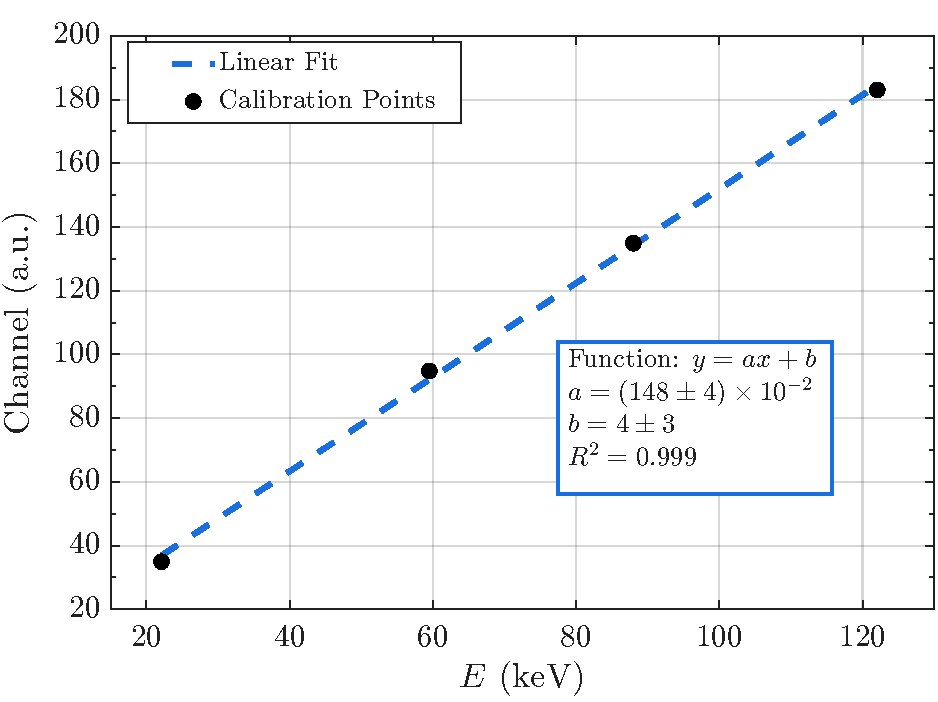
\includegraphics[width=0.47\linewidth]{images/fit_csi.pdf}}%
  \hfill%
  \subfloat[]{\label{fig:co57}%
    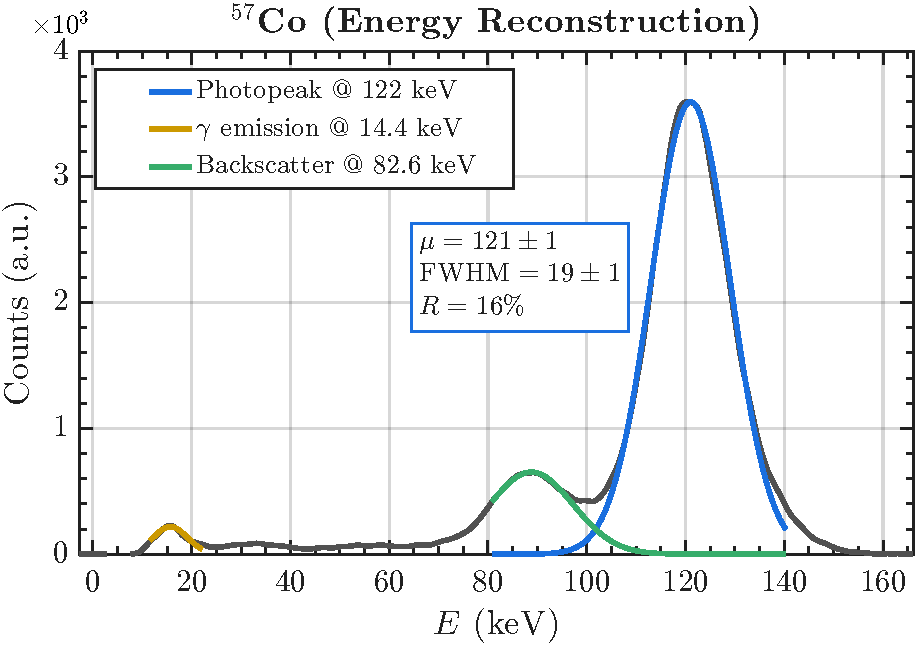
\includegraphics[width=0.50\linewidth]{images/co57_energy_reconstruction.pdf}}
  \caption[Validation of the Front-End Electronics.]{%
    \textbf{(a)} Pulse height spectra acquired with the CsI(Tl) crystal for the three calibration sources. Identified spectral features are labelled.
    \textbf{(b)} Channel-to-energy calibration curve with linear fit.
    \textbf{(c)} $^{57}$Co spectrum reconstructed in energy units.}
  \label{fig:validation_electronics}
\end{figure}

The centroid channel of each photopeak was mapped to its known energy value, and a linear fit of the form:
%
\begin{equation}
    C = aE + b,
    \label{eq:calibration_csi}
\end{equation}
%
was applied, where $C$ is the channel number and $E$ is the energy in keV (Fig.~\ref{fig:validation_electronics} (b)). The fit yields $R^2 = 0.999$, confirming a linear channel-to-energy relationship up to at least channel 183, corresponding to an input amplitude of approximately 590~mV. This confirms that the P\&H circuit does not introduce amplitude-dependent errors within this bin range.

As a validation of the calibration, the $^{57}$Co spectrum was reconstructed in energy units and is shown in Fig.~\ref{fig:validation_electronics} (c). The fitted centroid of the 122~keV photopeak yields $\mu = 121 \pm 1$~keV, consistent with the nominal value within uncertainty. The measured FWHM is $19 \pm 1$~keV, corresponding to an energy resolution of $16 \pm 1$\% at 122~keV, consistent with values reported in the literature for CsI(Tl)~\cite{117,118}. This indicates that the front-end electronics do not degrade the intrinsic energy resolution of the crystal. The DORI hardware is therefore considered validated.



\chapter{Calibration of the DORI Prototype}
\section{Energy Calibration}
\label{sec:energy_calibration}
As a novel approach for PSs, the energy response was calibrated using the \emph{Bremsstrahlung} endpoint of an X-ray tube. The maximum X-ray photon energy produced corresponds to the scenario in which the accelerated electron transfers all its kinetic energy in a single interaction with the anode nucleus. The maximum energy detected, i.e., the endpoint of the acquired spectrum, is therefore equal to the tube voltage, which serves as the energy reference for calibration. Since the \emph{Bremsstrahlung} spectrum near the endpoint is approximately linear, this abscissa can be determined as the $x$-intercept of a least-squares fit to that region~\cite{121}. This test and all subsequent tests relying on X-ray production used an Apogee 5500 Series tube (Oxford Instruments). It is 50~W tube that operates over a voltage range of 0 to 50~kV, with a maximum beam current of 1.0~mA~\cite{oxford2019apogee}.

The detector was positioned in the beam line, at a distance sufficient to avoid saturation of the front-end electronics. \emph{Bremsstrahlung} spectra were acquired over 5-minute intervals for tube voltages of 15--50~kVp and tube currents of 0.050--0.250~mA, and are shown in Fig.~\ref{fig:bremss_calibration} (a) and (b), respectively. Background was subtracted, and channels 18 and below were again excluded. As represented in Fig.~\ref{fig:bremss_calibration} (a), the 15~kVp spectrum is not visible, as it sits within the excluded background. At this distance and fluence, photons of such low energy are absorbed by the black adhesive tape used for light-wrapping of the photosensitive detector element. This establishes the lower bound of the calibrated range at 20~keV.
\begin{figure}[H]
  \centering
  \begin{minipage}[c]{0.48\linewidth}
    \centering
    \subfloat[]{\label{fig:bremss_spectra}%
      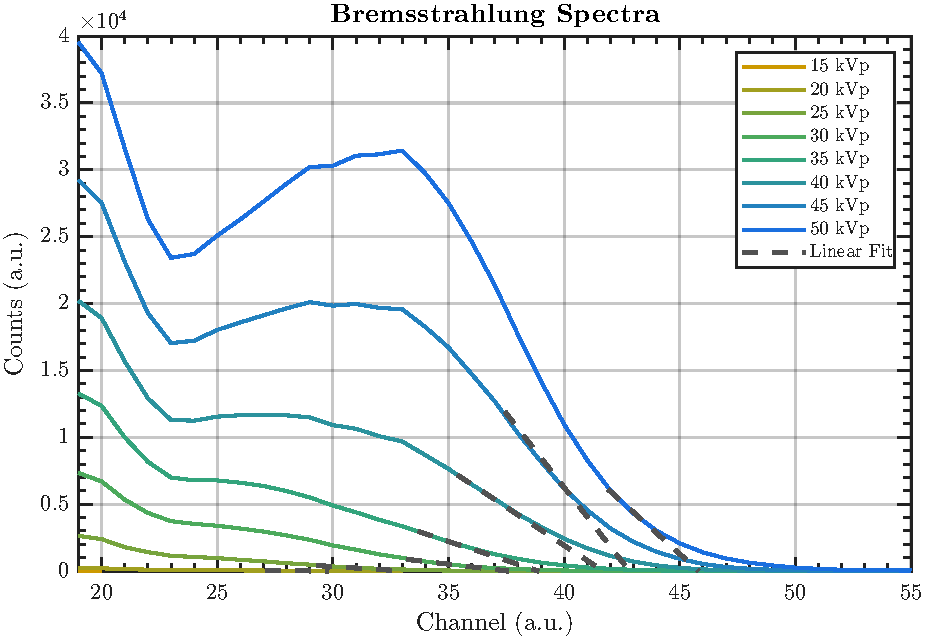
\includegraphics[width=\linewidth]{images/bremsstrahlung_fits.pdf}}
  \end{minipage}%
  \hfill%
  \begin{minipage}[c]{0.48\linewidth}
    \centering
    \subfloat[]{\label{fig:bremss_endpoint}%
      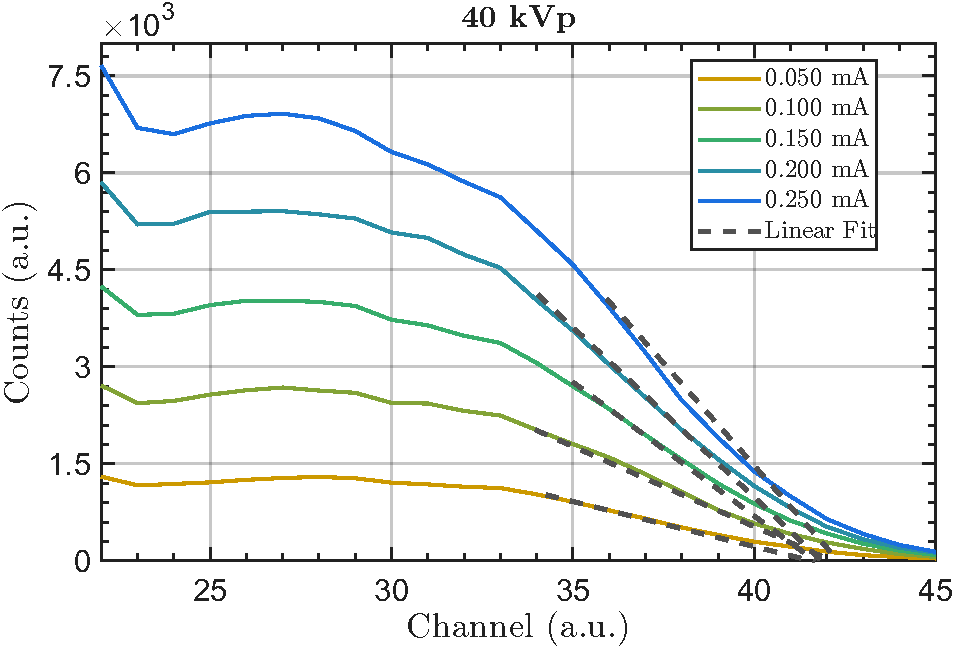
\includegraphics[width=\linewidth]{images/bremsstrahlung_40kVp_vs_current.pdf}}
  \end{minipage}
  \caption[\emph{Bremsstrahlung} Spectra.]{%
    \emph{Bremsstrahlung} spectra, background subtracted and excluded;
    \textbf{(a)} acquired at 0.250~mA for tube voltages from 15 to 50~kVp;
    \textbf{(b)} acquired at 40~kVp for tube currents from 0.050 to 0.250~mA.
  }
  \label{fig:bremss_calibration}
\end{figure}

The linear region of each \emph{Bremsstrahlung} spectrum was selected interactively, and a least-squares regression was applied to the points within that window. The $x$-intercept of the fitted line gives the endpoint channel. Since tube current affects only photon fluence and not the spectral endpoint, the five acquisitions per voltage produce five independent estimates (see Fig.~\ref{fig:bremss_calibration} (b)). The resulting values are summarized in Table~\ref{tab:endpoints}.

% Small vertical space after surrounding text
\vspace{1em}

% Manual table title, numbered and added to LoT
\refstepcounter{table}
\label{tab:endpoints}
\noindent\textbf{Table~\thetable.} \emph{Bremsstrahlung} endpoint channel for each tube voltage. Values are the mean of five acquisitions with the maximum deviation from the mean.
\addcontentsline{lot}{table}{\protect\numberline{\thetable}\emph{Bremsstrahlung} endpoint channel for each tube voltage.}

% Small space between title and table
\vspace{0.1em}

\begin{table}[H]
  \centering
  \begin{tabular}{>{\centering\arraybackslash}m{0.18\textwidth}
                  >{\centering\arraybackslash}m{0.08\textwidth}
                  >{\centering\arraybackslash}m{0.08\textwidth}
                  >{\centering\arraybackslash}m{0.08\textwidth}
                  >{\centering\arraybackslash}m{0.08\textwidth}
                  >{\centering\arraybackslash}m{0.08\textwidth}
                  >{\centering\arraybackslash}m{0.08\textwidth}
                  >{\centering\arraybackslash}m{0.08\textwidth}}
    \toprule
    \scriptsize \textbf{Tube Voltage (kVp)} & \scriptsize \textbf{20} & \scriptsize \textbf{25} & \scriptsize \textbf{30} & \scriptsize \textbf{35} & \scriptsize \textbf{40} & \scriptsize \textbf{45} & \scriptsize \textbf{50} \\
    \midrule
    \scriptsize \textbf{Endpoint Channel (a.u.)}
    & \scriptsize $31 \pm 3\%$
    & \scriptsize $33 \pm 3\%$
    & \scriptsize $37 \pm 1\%$
    & \scriptsize $39 \pm 1\%$
    & \scriptsize $42 \pm 1\%$
    & \scriptsize $43 \pm 1\%$
    & \scriptsize $45 \pm 2\%$ \\
    \bottomrule
  \end{tabular}
\end{table}
Although 20 and 25 keV lie in the boundary at which photoeletric absorption ceases to dominate in BC-408 (see Appendix~B), the associated uncertainty is dominated by counting statistics. The associated error improves between 30 and 45 keV, indicating that in this region both the photoelectric cross-section and the photon fluence are sufficient for the endpoint to be determined with good precision. At 50 keV, the photoelectric absorption in the scintillator drops below 0.5\%, and consequently the uncertainty increases. As full energy transfer becomes less probable, the spectrum compresses toward a lower and less reliable endpoint. Additionally, pileup further distorts the spectral shape near the abscissa. The pileup distortion is visible as a non-linear tail in the higher energy spectra of Fig.~\ref{fig:bremss_calibration} (a), which is not characteristic of filtered \emph{Bremsstrahlung}. At higher count rates, the baseline does not recover between successive pulses, causing them to superimpose and producing the observed tail. These are the fundamental limitations of the endpoint method at higher energies, as the associated uncertainty is expected to grow accordingly.

To extend the calibration beyond the range of the X-ray tube, spectra of the reference sources were acquired with the PS five times, each over a 90 min interval. Of the three sources, the only features available are the $^{241}$Am photopeak at 59.5 keV, and the CE of the 122 keV line of $^{57}$Co, at 39.46 keV, shown in Fig.~\ref{fig:source_spectra} (a) and (b) respectively. 
\begin{figure}[H]
  \centering
  \begin{minipage}[c]{0.50\linewidth}
    \centering
    \subfloat[]{\label{fig:Am-241}%
      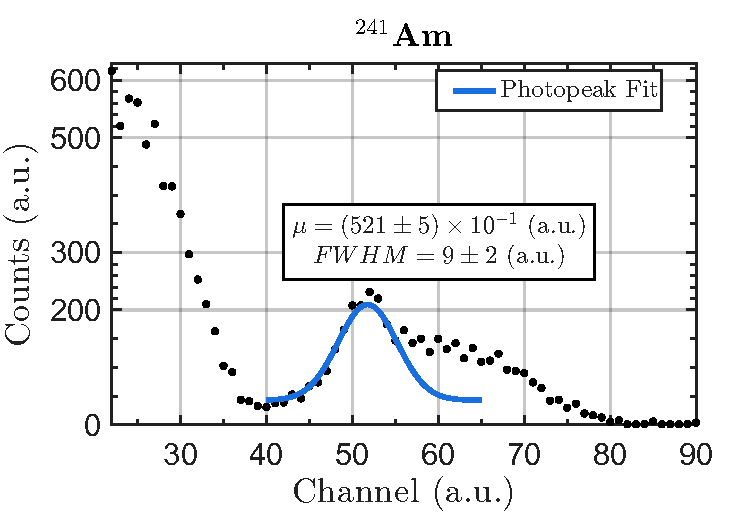
\includegraphics[width=\linewidth]{images/plastic_Am-241.pdf}}
  \end{minipage}%
  \hfill%
  \begin{minipage}[c]{0.50\linewidth}
    \centering
    \subfloat[]{\label{fig:Co-57}%
      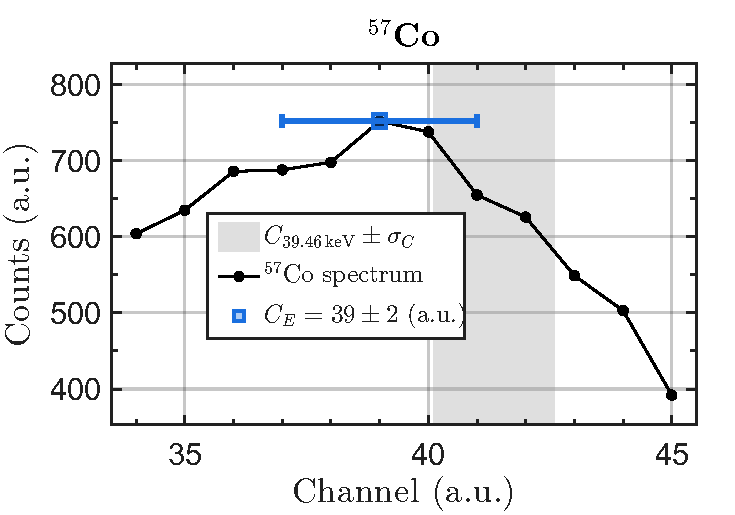
\includegraphics[width=\linewidth]{images/plastic_Co-57_fit.pdf}}
  \end{minipage}
  \caption[Reference source spectra.]{%
    Reference source spectra, background subtracted. Annotated values are the mean of five acquisitions with the maximum deviation from the mean as uncertainty.
    \textbf{(a)} $^{241}$Am, with the Gaussian fit to the 59.5~keV photopeak.
    \textbf{(b)} $^{57}$Co's Compton Edge at 39.46~keV.
  }
  \label{fig:source_spectra}
\end{figure}

The $^{241}$Am photopeak is fully resolved and was described by a Gaussian fit, whereas the $^{57}$Co CE was extracted as the channel of maximum counts. Despite the lower number of counts accumulated in the photopeak, it has the smaller uncertainty of the two features, and although it is not as sharp as the one obtained with the CsI crystal in Section~\ref{sec:frontend-validation}, the centroid position is reproducible across acquisitions. The broadening of the $^{57}$Co feature is a consequence of the energy dependence of the resolution and its degradation at lower energies. The photopeak is therefore included as a calibration point at 59.5~keV, whereas the edge, falling within the interval already covered by the tube, is treated as an independent validation of the \emph{Bremsstrahlung} method.

A weighted least-squares fit was applied to account for the differences in uncertainty across the energy range and is shown in Fig.~\ref{fig:energy_calibration}.
\begin{figure}[H]
  \centering
  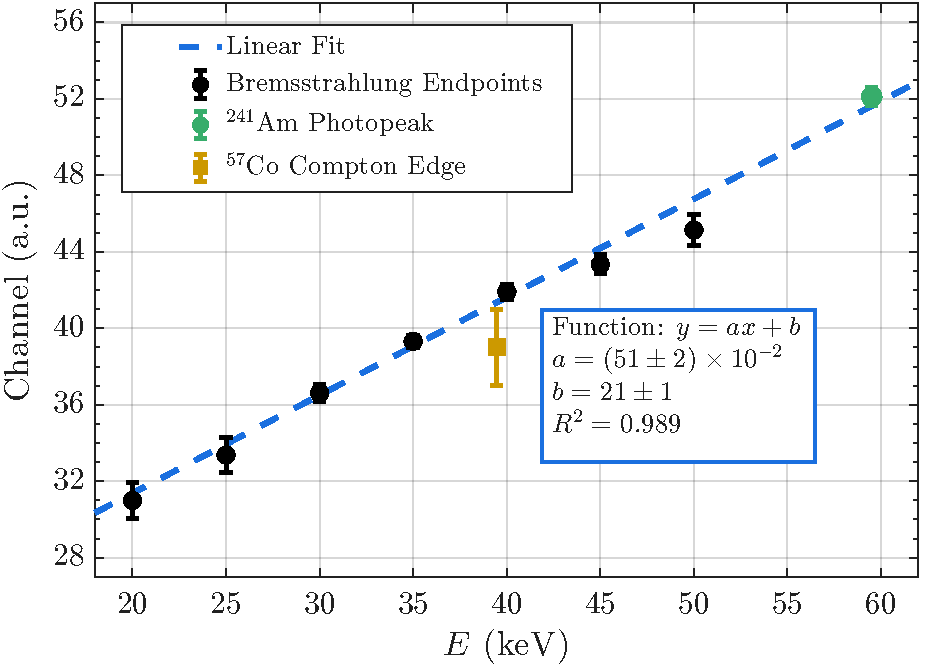
\includegraphics[width=0.85\linewidth]{images/energy.pdf}
  \caption[Energy calibration of the DORI prototype.]{%
    Weighted least-squares energy calibration of the DORI prototype, obtained from the seven \emph{Bremsstrahlung} endpoints and the $^{241}$Am photopeak centroid. The $^{57}$Co Compton edge is superimposed for validation.
  }
  \label{fig:energy_calibration}
\end{figure}
Although the 45 keV uncertainty is small, both the 45 and 50 keV endpoints fall below the calibration line, beyond their uncertainties. This underestimation is consistent with the compression of the spectrum discussed above. In contrast, the $^{241}$Am centroid falls on the calibration line with an uncertainty smaller than that of the highest-energy endpoint estimate. The weighted fit ensures that these better-determined points contribute more to the calibration, and the uncertainties in each estimate propagate into the calibration coefficients~\cite{121}. The fit is of the form:
\begin{equation}
    C = aE + b,
    \label{eq:calibration}
\end{equation}
where $C$ is the channel number and $E$ is the energy in keV. With $R^2 = 0.989$, the DORI response can be treated as locally linear within the calibrated interval of 20 to 60 keV. Given a measured channel, the energy is therefore obtained from the following simplified expression~\cite{125}:
\begin{equation}
    E = \frac{C - 21}{0.51},
    \label{eq:energy_conversion}
\end{equation}
\begin{equation}
    \sigma_E = \frac{1}{0.51}\sqrt{(0.02)^2\,E^2 + 1^2}.
    \label{eq:energy_uncertainty}
\end{equation}


The $^{241}$Am photopeak in Fig.~\ref{fig:source_spectra} (a) has a FWHM of $9 \pm 2$ channels, above the minimum of five channels set in Section~\ref{sec:shaping}. The chosen gain therefore samples the photopeak adequately. As the only available photopeak, its centroid is also used to calculate the energy resolution of the DORI system at 59.5 keV. Although $R$ is dimensionless and, in principle, independent of the channel-to-energy conversion, the non-zero intercept $b$ shifts the centroid without contributing to the FWHM. Consequently, the resolution differs between channel and energy space and these parameters must be converted to energy using Eqs.~\ref{eq:energy_conversion} and \ref{eq:energy_uncertainty}. With these values, DORI has an energy resolution of $R = (29 \pm 5)$\% at 59.5 keV, consistent with values reported in the literature, and previously discussed, for BC-408 PSs. 

As for the CE of the 122~keV line of $^{57}$Co, the extracted channel falls below the calibration line, outside of it even within its own uncertainty. This discrepancy was predicted in Section~\ref{sec:scintillator} and is attributed to the extraction method rather than to the calibration itself. According to Swiderski~\emph{et al.}~\cite{127}, the finite resolution of PSs causes the channel of maximum counts not to coincide with the true position of the edge. The CE lies at a channel above that of maximum counts, and the offset grows as the resolution degrades. Taking CE as the maximum of the distribution therefore introduces a systematic and observed underestimation. The deviation is thus not evidence of a failure of the \emph{Bremsstrahlung} calibration, although the extraction method does not allow it to be validated either. Additionally, extension of the linear fit to 100 keV cannot be assumed, as it would span the non-proportional region of the plastic response discussed in Section~\ref{sec:scintillator}. In the absence of additional calibration points, the gap between 60 and 100 keV is acknowledged as a limitation of the present calibration. Within these limits, the DORI prototype response across the 20 to 60 keV range is characterized and the following dose calibration is performed within this interval.

\section{Dose Calibration}
\label{sec:dose_rate_calibration}

As introduced, an individual monitoring device is calibrated in personal dose equivalent, $H_p(d)$, with $d = 10$~mm adopted, the depth at which the quantity is defined for whole-body exposure. These devices are calibrated in certified laboratories, which have reference instruments and ensure the reproducibility and traceability of the measurements. The available reference fields include radionuclide sources, mono-energetic X-radiation and continuous filtered X-ray beams of defined quality, and conversion coefficients are provided for all of them. The calibration presented here follows the ISO 4037 series~\cite{113,ISO2,ISO3} for the conversion of \emph{air KERMA} to $H_p(10)$, using filtered X-ray beams of the narrow (N) series, the same reference qualities over which the commercial RaySafe i3 is calibrated. The protocol was adapted to the instrumentation available with the intention of demonstrating the methodology and showing that DORI can be calibrated as a prototype.

\subsection{Setup}
The production of the radiation quality needed depends on the tube potential, the total filtration and the properties of the anode. Given the X-ray tube available and the energy calibration, only radiation qualities with energies in the 20 to 50~keV range can be used. In the N-series that corresponds to N-25, N-30 and N-40, as the N-20 spectrum falls outside the calibrated energy range. The parameters defining each of the three qualities, together with the corresponding conversion coefficients, are listed in Table~\ref{tab:nseries}.
% Small vertical space after surrounding text
\vspace{1em}

% Manual table title, numbered and added to LoT
\refstepcounter{table}
\label{tab:nseries}
\noindent\textbf{Table~\thetable.} N-series radiation qualities. Coefficients correspond to the ISO slab phantom at 1-meter normal incidence. Adapted from Refs.~\cite{113,ISO3}.%
\addcontentsline{lot}{table}{\protect\numberline{\thetable}N-series radiation qualities.}

% Small space between title and table
\vspace{0.1em}

\begin{table}[H]
  \centering
  \begin{tabular*}{\textwidth}{@{\extracolsep{\fill}}cccc@{}}
    \toprule
    \textbf{\begin{tabular}[b]{@{}c@{}}Radiation\\Quality\end{tabular}} &
    \textbf{\begin{tabular}[b]{@{}c@{}}Tube Potential\\(kVp)\end{tabular}} &
    \textbf{\begin{tabular}[b]{@{}c@{}}Added\\Filtration\end{tabular}} &
    \begin{tabular}[b]{@{}c@{}}$\bm{h_{pK}(10)}$\\\textbf{(Sv/Gy)}\end{tabular} \\
    \midrule
    \textbf{N-25} & 25 & 2 mm Al & 0.574 \\
    \textbf{N-30} & 30 & 4 mm Al & 0.815 \\
    \textbf{N-40} & 40 & 4 mm Al + 0.21 mm Cu & 1.210 \\
    \bottomrule
  \end{tabular*}
\end{table}
As introduced, the dosimeter must be placed on a PMMA phantom during the calibration. For $H_p(10)$ the ISO water slab phantom is used, since it reproduces the backscatter of the trunk of the body and therefore the conditions under which the dosimeter is worn for this specific quantity. It consists of a PMMA shell of 30 $\times$ 30 $\times$ 15~cm, with a 2.5~mm front wall and 10~mm remaining walls, filled with water~\cite{ISO3}. A phantom replicating these dimensions was built for this work, but it was not filled with water, due to the risk of leakage in the presence of electronics around the setup. The DORI-test board was taped to the front wall of the phantom, with its photosensitive area aligned with the centre of the tube. Custom 3D-printed supports were made to hold the filters, and these sit on an alignment rail together with the phantom. The setup is shown in Fig.~\ref{fig:setup}. The centre of the PS entrance face is placed 1~meter away from the tube, and this position is taken as the reference measurement point, marked by the red star in the image. The \emph{air KERMA} was measured with the R/F Low detector of the RaySafe Xi~\cite{raysafe}, which was the only one to provide a measurable signal at this distance. The instrument was last calibrated in October 2013 and the product has since been discontinued, however, it was the only reference available. For these measurements the phantom and the dosimeter are removed from the rail and the centre of the R/F Low detector is placed at the reference point. 

It should be noted that the reference conditions under which the conversion coefficients of Table~\ref{tab:nseries} are defined cannot be fully reproduced with the available instrumentation. The phantom was not filled with water, so the backscatter contribution is lower than the one assumed by the standard. The anode is made of molybdenum instead of tungsten, although its characteristic lines lie below the calibrated energy range and therefore do not contribute to the measured spectra. The inherent filtration falls only within the maximum deviation permitted by ISO 4037, and the HVL of each quality were not tracked. Most importantly, the main limitation is the reference instrument itself. The values obtained are therefore not traceable and the procedure described here does not constitute a formal calibration. Its purpose is to establish and validate a methodology that reproduces the ISO 4037 framework as closely as the available setup allows, so that the same procedure can later be planed and repeated at a certified facility under the required field conditions. 
\begin{figure}[H]
  \centering
  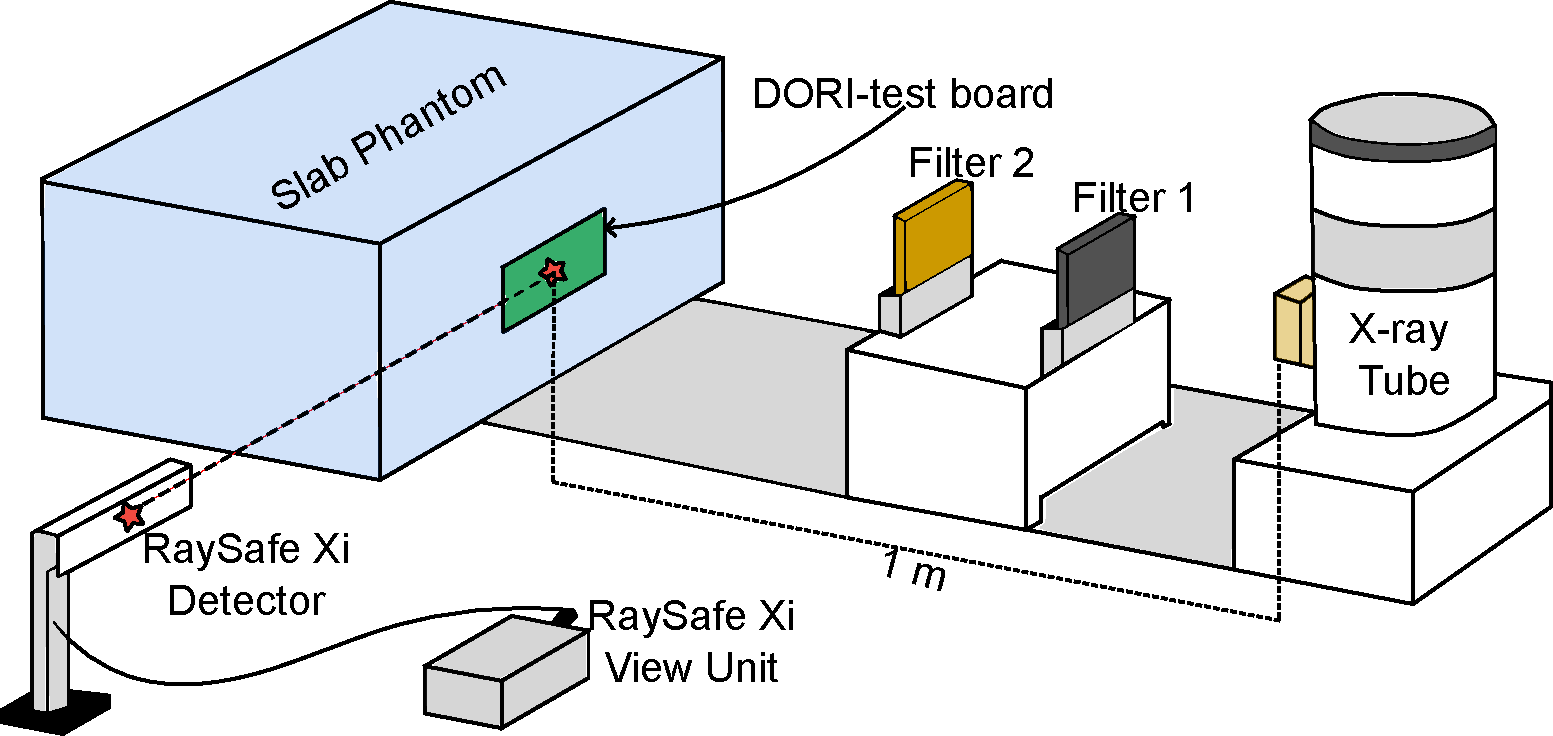
\includegraphics[width=\linewidth]{images/dose.pdf}
  \caption[Dose calibration setup.]{Dose calibration setup. The beam quality is defined by the placement of one filter, or two in the case of N-40, at the exit window of the X-ray tube. The DORI-test board is placed at the reference measurement point (red star), in contact with the front wall of the built slab phantom. The RaySafe Xi detector is positioned at the same point of test free in air, with the phantom removed, and the \emph{air KERMA} values are read on its view unit.}
  \label{fig:setup}
\end{figure}



All acquisitions were made at a tube current of 0.5~mA for 2 minutes, and the spectrum and average \emph{air KERMA} rate from DORI and the RaySafe were recorded, respectively.
The spectra acquired are shown in Fig.~\ref{fig:dose}~(a). Counts below the lower limit of the validated energy calibration and above the endpoint energy of the respective beam were excluded. Each spectrum is therefore confined to its expected energy range, and noise and pile-up events are rejected.

\begin{figure}[H]
  \centering
  \begin{minipage}[c]{0.50\linewidth}
    \centering
    \subfloat[]{\label{fig:dose_spectra}%
      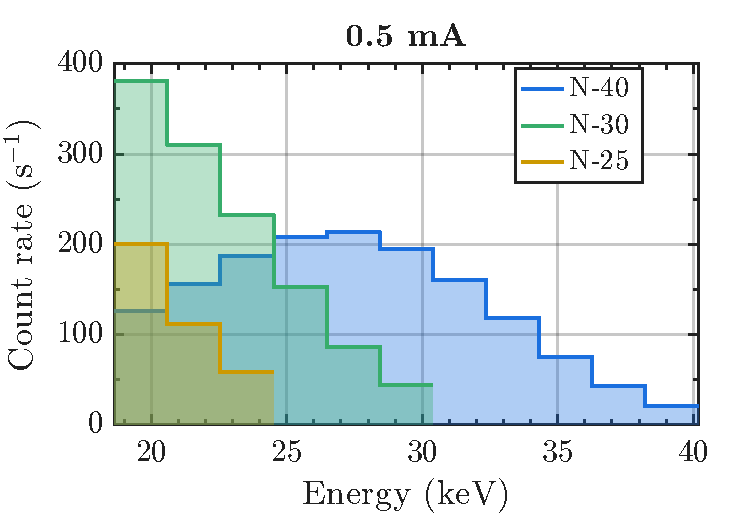
\includegraphics[width=\linewidth]{images/fig1_spectra.pdf}}
  \end{minipage}%
  \hfill%
  \begin{minipage}[c]{0.50\linewidth}
    \centering
    \subfloat[]{\label{fig:hp_10}%
      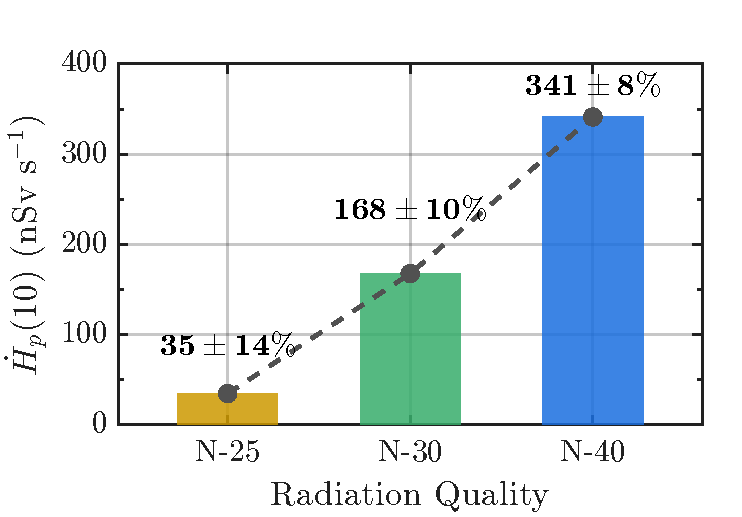
\includegraphics[width=\linewidth]{images/fig2_reference.pdf}}
  \end{minipage}
  \caption[ISO 4037 narrow-series qualities N-25, N-30 and N-40, acquired at 0.500~mA for 2 minutes.]{ISO 4037 narrow-series qualities N-25, N-30 and N-40, acquired at 0.500~mA for 2 minutes.
    \textbf{(a)} Energy spectra;
    \textbf{(b)} reference $\dot{H}_p(10)$.
  }
  \label{fig:dose}
\end{figure}

The effect of the filtration can be seen, since all acquisitions were made at the same tube current and for the same duration. Without filtration, the count rate would scale approximately with the square of the tube potential. The N-series filtration is designed to narrow the spectrum by suppressing its low-energy component. The lower count rate registered at the lower energies for N-40 is a direct consequence of the copper filter. This is not seen for N-30. N-30 requires twice the aluminium of N-25 and yet exceeds it at every energy the two share, since the higher output of the harder beam compensates the additional attenuation. The low-energy component of N-40 is nevertheless not completely suppressed. The detected counts originate from Compton interactions in the PS and from photons scattered by the slab phantom, which is itself intended to produce scattering. As a consequence, the mean energy of each distribution falls progressively below the value tabulated by ISO for the corresponding quality.

The reference $\dot{H}_p(10)$ obtained for each quality is shown in Fig.~\ref{fig:dose}(b), calculated from the measured \emph{air KERMA} rate and the conversion coefficients of Table~\ref{tab:nseries}. The values increase with tube potential, as both terms of the product grow with beam energy. The relative uncertainty decreases with tube potential, from $14\%$ at N-25 to $8\%$ at N-40. The \emph{air KERMA} rates of N-30 and N-40 sit above the trigger level of the detector ($>100$~nGy~s$^{-1}$)~\cite{Specs}, while that of N-25 is flagged as a low signal, contributing to the higher uncertainty.

\subsection{Methods}

The absorbed dose increases with the energy deposited, so counts registered at different energies do not produce the same biological effect. $H_p(10)$ can therefore be written as a sum over the spectrum, each count contributing according to the energy at which it was detected:
\begin{equation}
H_p(10) = \sum_{i=1}^{m} w_i N_i ,
\label{eq:bin_model}
\end{equation}
where $N_i$ is the number of counts and $w_i$ the dose per count, in Sv/count.  Each weight holds the response of DORI to the ISO reference field in that energy range, since it converts the counts the device registers into the dose delivered. Calibrating the dosimeter in dose therefore corresponds to determining the set of weights $w_i$.
 
As shown, each radiation quality produces one pulse height spectrum with an associated $H_p(10)$ rate. Since the radiation is not monoenergetic, the weights cannot be assigned to individual energies. The spectrum must instead be grouped into $m$ bins, each covering a range of energies which will carry the same weight. The number of bins that can be resolved is limited by the number of radiation qualities available, as each quality provides one equation of the form of Eq.~\ref{eq:bin_model}. For $q$ radiation qualities, the measurements can be written as:
\begin{equation}
\begin{bmatrix}
H_1 \\ H_2 \\ \vdots \\ H_q
\end{bmatrix}
=
\begin{bmatrix}
N_{11} & N_{12} & \cdots & N_{1m} \\
N_{21} & N_{22} & \cdots & N_{2m} \\
\vdots & \vdots  & \ddots & \vdots \\
N_{q1} & N_{q2} & \cdots & N_{qm}
\end{bmatrix}
\begin{bmatrix}
w_1 \\ w_2 \\ \vdots \\ w_m
\end{bmatrix},
\label{eq:system}
\end{equation}
where each row of $\mathbf{A}$ holds the counts per bin measured for one quality, $\mathbf{H}$ is the measured $H_p(10)$ and $\mathbf{w}$ the unknown weights. For $q > m$ the system is overdetermined and is solved by the least-squares method~\cite{portable}:
\begin{equation}
\mathbf{w} = \left(\mathbf{A}^{\!\top}\mathbf{A}\right)^{-1}
\mathbf{A}^{\!\top}\mathbf{H} .
\label{eq:lsq}
\end{equation}

With three radiation qualities available, $q = 3$ and the system of Eq.~\ref{eq:system} admits at most three unknowns. Solving it with $m = 3$ fits the three measurements exactly, leaving no redundancy with which to verify the solution and making no use of the uncertainties of the reference values. Choosing $m = 2$ leaves one degree of freedom, which allows a weighted solution and leaves a residual against which the quality of the fit can be assessed. For this case, the counts of every quality are summed into two groups separated by a single boundary. Eleven channels cover the 20 to 40~keV range, so ten boundary positions are possible. All of them were tested and the two most representative cases are shown in Fig.~\ref{fig:weights}~(a) and (b), the division at 25~keV and the equal-width division at 30~keV, respectively.

\begin{figure}[H]
  \centering
  \begin{minipage}[c]{0.48\linewidth}
    \centering
    \subfloat[]{\label{fig:w_2bin25}%
      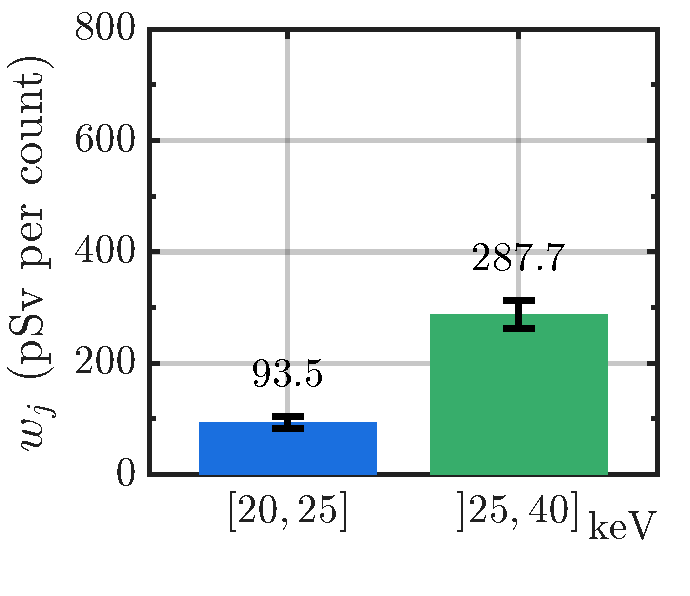
\includegraphics[width=\linewidth]{images/weights2bin25_sub.pdf}}
  \end{minipage}%
  \hfill%
  \begin{minipage}[c]{0.48\linewidth}
    \centering
    \subfloat[]{\label{fig:w_2bin30}%
      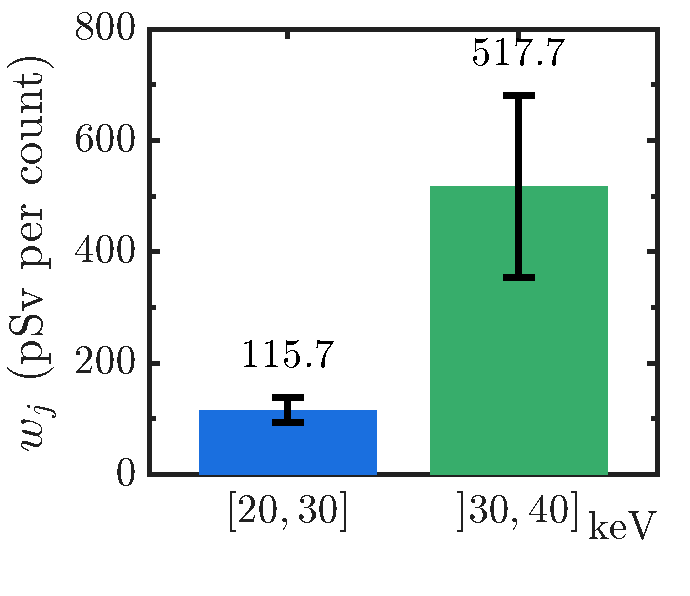
\includegraphics[width=\linewidth]{images/weights2bin30_sub.pdf}}
  \end{minipage}

  \vspace{1em}
  \begin{minipage}[c]{0.85\linewidth}
    \centering
    \subfloat[]{\label{fig:w_3bin}%
      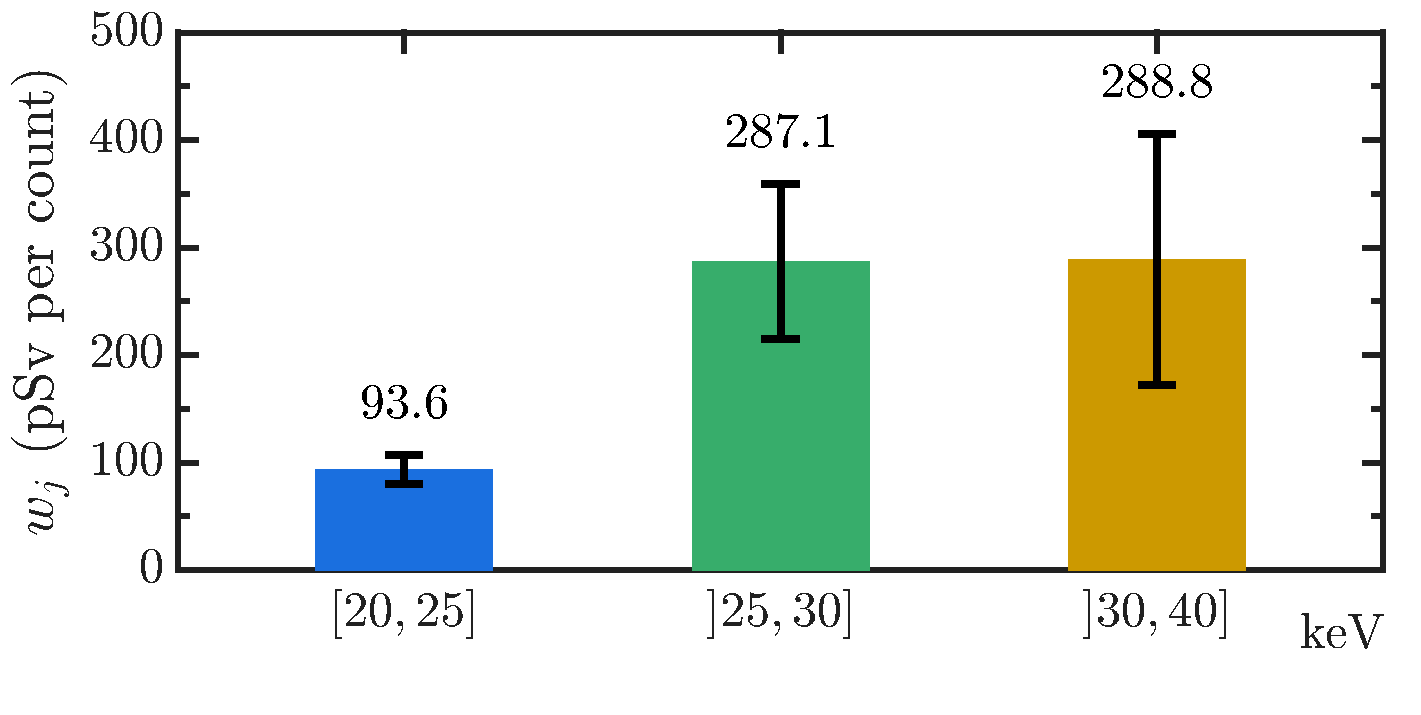
\includegraphics[width=\linewidth]{images/weights3bin_sub.pdf}}
  \end{minipage}
  \caption[Dose per count obtained for three binning schemes.]{Dose per count obtained for three binning schemes within the calibrated 20 to 40~keV range.
    \textbf{(a)} Two bins divided at 25~keV;
    \textbf{(b)} two bins divided at 30~keV;
    \textbf{(c)} three bins divided at 25 and 30~keV.
  }
  \label{fig:weights}
\end{figure}


Both divisions return $w_2 > w_1$, as expected from the increase of dose with the energy detected, but they differ in how well each weight is determined. At 25~keV the boundary coincides with the end of the N-25 spectrum. N-25 therefore falls entirely in the lower bin and fixes $w_1$ by itself, while N-30 and N-40 both populate the upper bin and together determine $w_2$. Every quality is used, and the uncertainties obtained are the lowest of the three schemes. For any boundary above this energy, N-25 and N-30 both contribute to the lower bin, and for these cases, most notably at 30~keV, the two qualities have incompatible values of $w_1$, $93.6$ and $139.0$~pSv/count respectively. The solution is therefore a compromise between the two. Additionally, and as represented for this specific scenario, the uncertainty of $w_2$ is the largest, which makes this division unsuitable.

The small number of measurements also allows the solution to be determined directly. As mentioned in the last paragraph, since N-25 has no counts in the upper bin, it determines $w_1$ on its own, $93.6 \pm 13.2$~pSv/count. Subtracting that contribution from N-30 gives $w_2 = 287.1 \pm 72.0$~pSv/count over the 25 to 30~keV range, and subtracting both contributions from N-40 gives $w_3 = 288.8 \pm 116.9$~pSv/count over the 30 to 40~keV range. Two independent radiation qualities therefore return the same weight, within the uncertainty of the fit, and the increase expected for the third weight is marginal and lies only within its uncertainty. This reasoning is the three-bin solution represented in Fig.~\ref{fig:weights}~(c). For this scenario, the uncertainties of the two upper weights increase to $25\%$ and $40\%$ against $10\%$ in the two-bin solution, which makes the model less robust.

A two-bin model was therefore adopted, with $N_1 \in \left[20,25\right]$~keV and $N_2 \in \left]25,40\right]$~keV, and Eq.~\ref{eq:bin_model} reduces to:
\begin{equation}
H_p(10) = w_1 N_1 + w_2 N_2 ,
\label{eq:two_bin}
\end{equation}
with the values in Fig.~\ref{fig:weights}~(a):
\begin{equation}
w_1 = 93.5 \pm 11.4, \qquad w_2 = 287.7 \pm 25.5,\ \text{unit: } \left[\frac{\mathrm{pSv}}{\mathrm{count}}\right] .
\label{eq:weights}
\end{equation}
 
\noindent A count registered in the upper bin therefore carries $3.1$ times the dose of a count registered in the lower bin, which translates the effect of higher energy on the dose delivered. It should be noted that a 15~keV bin is broad considering the available range, but it is again a consequence of the small number of radiation qualities that can be used. A tube capable of higher potentials would provide additional qualities and allow finer divisions. Given a measured spectrum, the personal dose equivalent is therefore obtained from the following simplified expression:
\begin{equation}
    H_p(10) = 93.5\,N_1 + 287.7\,N_2 ,
    \label{eq:dose_conversion}
\end{equation}
\begin{equation}
    \sigma_{H_p(10)} = \sqrt{\left(11.4\,N_1\right)^2 + \left(25.5\,N_2\right)^2} ,
    \label{eq:dose_uncertainty}
\end{equation}

The response of DORI after calibration is shown in Table~\ref{tab:response}, where the reconstructed ${H}_p(10)$ agrees with the reference value within the uncertainty, for the three qualities and for both reconstructions. The calibration therefore reproduces the measurements from which it was derived. Additionally, a leave-one-out test was performed, where the weights are recomputed from two qualities and used to predict the $\dot{H}_p(10)$ of the third by reconstructing the dose from its own bin counts. The most interesting result is the case of N-25. As mentioned, it is the only direct measurement of $w_1$. When excluded, $w_1$ can only be inferred from the different proportions in which N-30 and N-40 divide their counts between the two bins. As can be seen, the reconstructed dose differs by approximately $0.3\%$, indicating that $w_1$ is well determined by the available measurements and is not an artefact of the single quality that defines it.

Overall, these results support the two-bin model and the position of its boundary, and indicate that, with the three measurements available, this was the best division that could be made. The precision of the calibration is limited not only by the number of qualities, but also by the uncertainty of the reference dose values, which is dominated by the RaySafe Xi for the reasons already given. It should be emphasised that a formal calibration was never the purpose. The goal of demonstrating that a prototype of this kind can be calibrated in dose from its own spectrum has been achieved, and the methodology is shown to be workable. A significant part of the future work will therefore be to extend the energy calibration to higher energies and to obtain more reliable $\dot{H}_p(10)$ reference values.

\vspace{1em}
\refstepcounter{table}
\label{tab:response}
\noindent\textbf{Table~\thetable.} Reference $\dot{H}_p(10)$ and the values reconstructed by the two-bin calibration and by the leave-one-out test, for the three radiation qualities.
\addcontentsline{lot}{table}{\protect\numberline{\thetable}Response of DORI after the dose calibration.}

\vspace{0.1em}
\begin{table}[H]
  \centering
  \begin{tabular*}{\textwidth}{@{\extracolsep{\fill}}cccc@{}}
    \toprule
    \textbf{\begin{tabular}[b]{@{}c@{}}Radiation\\Quality\end{tabular}} &
    \textbf{\begin{tabular}[b]{@{}c@{}}Reference\\(nSv s$^{-1}$)\end{tabular}} &
    \textbf{\begin{tabular}[b]{@{}c@{}}Calibration\\(nSv s$^{-1}$)\end{tabular}} &
    \textbf{\begin{tabular}[b]{@{}c@{}}Leave-one-out\\(nSv s$^{-1}$)\end{tabular}} \\
    \midrule
    \textbf{N-25} & $35 \pm 5$   & $35 \pm 4$  & $35 \pm 8$ \\
    \textbf{N-30} & $168 \pm 16$ & $168 \pm 13$ & $168 \pm 14$ \\
    \textbf{N-40} & $341 \pm 26$ & $341 \pm 27$ & $340 \pm 75$ \\
    \bottomrule
  \end{tabular*}
\end{table}




\section{Dose Rate Reconstruction}
\label{sec:dose_rate}

The spectra acquired for the energy calibration were reprocessed through the two-bin dose calibration. Each spectrum was cut at its own \emph{Bremsstrahlung} endpoint, and only tube potentials of 25, 30, 35 and 40~kVp were used, as they sit within the calibrated energy range. The resulting dose rates, for five tube currents at each of the four potentials, are shown in Fig.~\ref{fig:dose_linearity}. 

\begin{figure}[H]
  \centering
  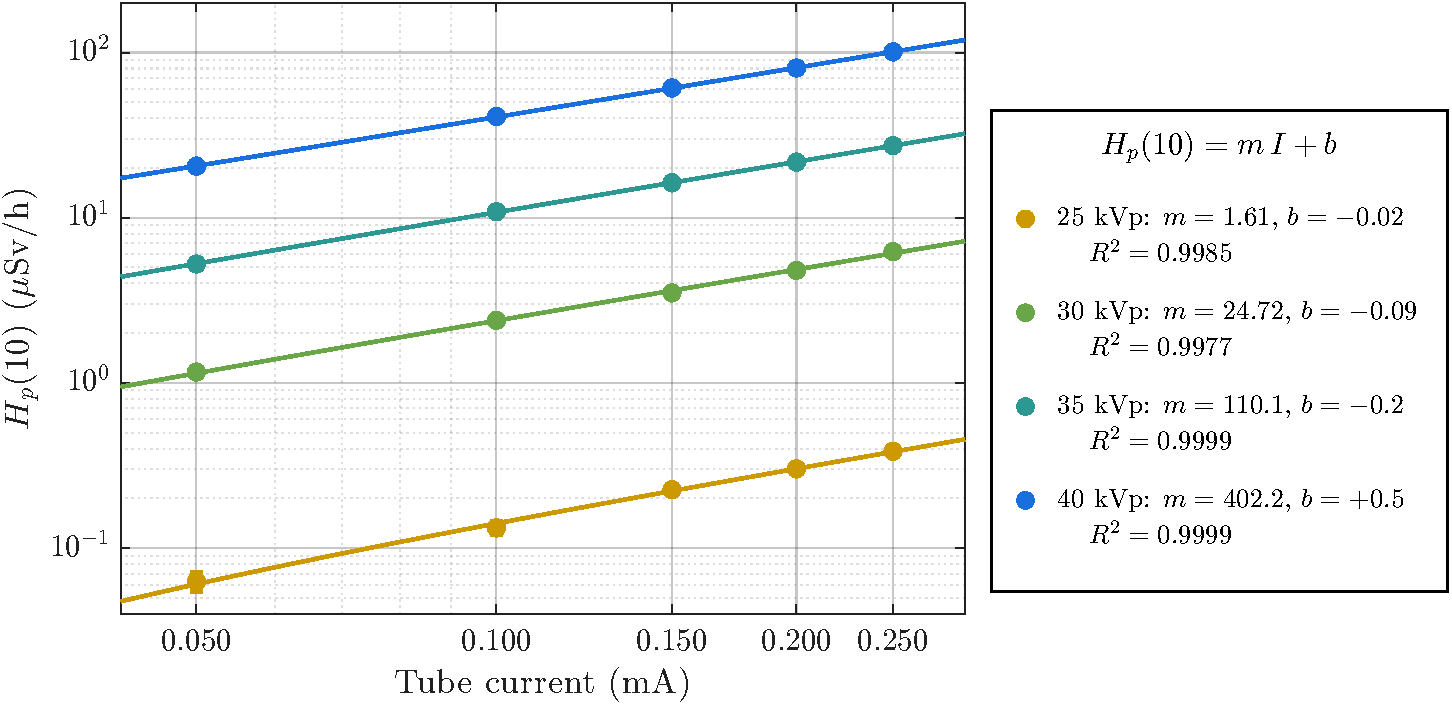
\includegraphics[width=1\linewidth]{images/dose_rate_linearity.pdf}
  \caption[Reconstructed $H_p(10)$ rate as a function of tube current.]{Reconstructed $H_p(10)$ rate as a function of tube current, for tube
potentials of 25-40~kVp and currents of 0.050-0.250~mA.
  }
  \label{fig:dose_linearity}
\end{figure}

The measurements span 0.063 to 101~$\mu$Sv/h. At every tube potential the dose rate increases linearly with the tube current, with $R^2 \geq 0.998$. The fitted intercepts are consistent with zero at all four potentials, as expected, since no tube current means no counts and therefore no dose. The largest deviation from the fitted line is $6\%$, occurring at 25~kVp, and is attributed to the poorer counting statistics at this potential. The total count rate over the whole set ranges from 82 to $1.9\times10^{3}$~s$^{-1}$, against the saturation count rate of $56\times10^{3}$~s$^{-1}$ given in Section~\ref{sec:pulse_sampling}. The measurements therefore lie within a reliable photon counting region, where dead time and pile-up are negligible. The ratio $N_2/N_1$ remains constant with the tube current at the potentials where both bins are populated, indicating that the distribution of counts is preserved over this range. 

The relevance of this range can be assessed against the isodose map of Fig.~\ref{fig:scatter}, keeping in mind that the reliability of the reconstructed values depends on the assumptions of the dose calibration described in the previous section. That map spans 0.0075 to 167~$\mu$Sv/h behind a lead apron and 0.5 to $12\times10^{3}$~$\mu$Sv/h without one, at chest level, for one of the most demanding procedures in this modality. The range reconstructed here overlaps most of the shielded scale, but covers only the lower part of the unshielded one, which are detected at higher scattering distances. Other studies report average dose rates of approximately 30~$\mu$Sv/h for conventional interventions above personal shielding~\cite{53}. The dose rates are therefore relevant, but the position at which the dosimeter is worn should be considered when a full energy and dose calibration is defined. The limit in count rate has also not been established, and the performance of the prototype has to be characterised before an operating range in dose rate can be claimed. Reaching those rates would involve higher photon energies, and establishing the limit of linearity requires, once again, a more complete energy and dose calibration.









\chapter{Final Prototype}

The current DORI prototype is shown in Fig.~\ref{fig:prototype}.
A new PCB was designed with emphasis on a more compact footprint, correcting the layout errors identified in the DORI-test board and optimised for wireless operation. In comparison with the previous PCB, the colour-coded LED was integrated, and a power switch was added to disconnect the LiPo battery from the circuit. Additionally, all oscilloscope test points were removed and the SiPM is now soldered directly onto the board.

To obtain a portable version of the system, and to ensure that no ambient light reaches the photosensitive elements, a two-part 3D printed case was designed. The lower layer contains a dedicated compartment for the LiPo battery (Fig.~\ref{fig:prototype}~(a)) and is enclosed by the PCB. As shown in Fig.~\ref{fig:prototype}~(b), the PS was wrapped in several layers of Teflon tape, covering all non-exiting surfaces of the cube. Optical silicone grease(!!!!!!!) was applied as coupling between the SiPM and the PS. The friction it creates, together with dedicated holes in the top layer of the case, keep the PS in place and aligned with the SiPM. Apertures are provided for the LED, the power switch (Fig.~\ref{fig:prototype}~(c)) and the USB-C port for charging and firmware uploading. The top layer is closed tightly against the bottom one with four screws. A loop was modelled on the top to hold a standard badge clip, allowing the unit to be worn over clothing. As represented, the current DORI unit measures 6.3~cm in width, 7.2~cm in height and 2.5~cm in thickness, with a total mass of 141~g. For comparison, the RaySafe i3 device measures 4.0 $\times$ 5.8 $\times$ 1.7~cm and has a mass of only 34~g. Although the dimensions are comparable, the DORI PCB still leaves room for improvement in size, through a better use of the PCB's top and bottom layers for component placement. Additionally, the integration of the ESP32-C3 as a bare chip, rather than the prototyping module, would contribute further to the reduction of the footprint. From a wearable point of view, the mass is currently the most likely cause of discomfort. The enclosure was printed at 100\% infill to guarantee that no ambient light reaches the photosensitive elements. This choice increases the mass of the unit, which is higher than desirable for a badge worn over clothing. If light-tightness can be preserved, a reduction can be achieved with a lower infill density, or with different printing methods and materials.

All design files of the final prototype are made available in a public repository [repository link], so that the system can be reproduced and further developed. These include the CAD models of the enclosure, the PCB layout and schematic, the firmware, the acquisition software and the energy and dose calibration parameters derived in this work. Future work should also include the implementation of the graphical user interface projected in Chapter~\ref{chapter:hardware_development}, for real time visualisation of the dose rate and storage of the acquired data.

\begin{figure}[H]
  \centering
  \resizebox{1\linewidth}{!}{\begin{tikzpicture}[x=1pt,y=1pt,
    every node/.style={font=\footnotesize},
    ah/.style={draw opacity=0,line width=0.08,fill opacity=1},
    ahs/.style={ah,scale=0.55},
    lbl/.style={fill=white,align=center,inner sep=2.5pt,line width=0.6pt},
    dim/.style={fill=white,align=center,inner sep=2pt,draw=none,font=\scriptsize},
    pan/.style={font=\footnotesize\bfseries,inner sep=0pt,anchor=north}]

% =========================================================================
% (a)  bottom shell  --  image x: 59.5 -> 237.25 , y: 172 -> 308.9
% =========================================================================
\node [anchor=south west,inner sep=0] at (59.5,172)
  {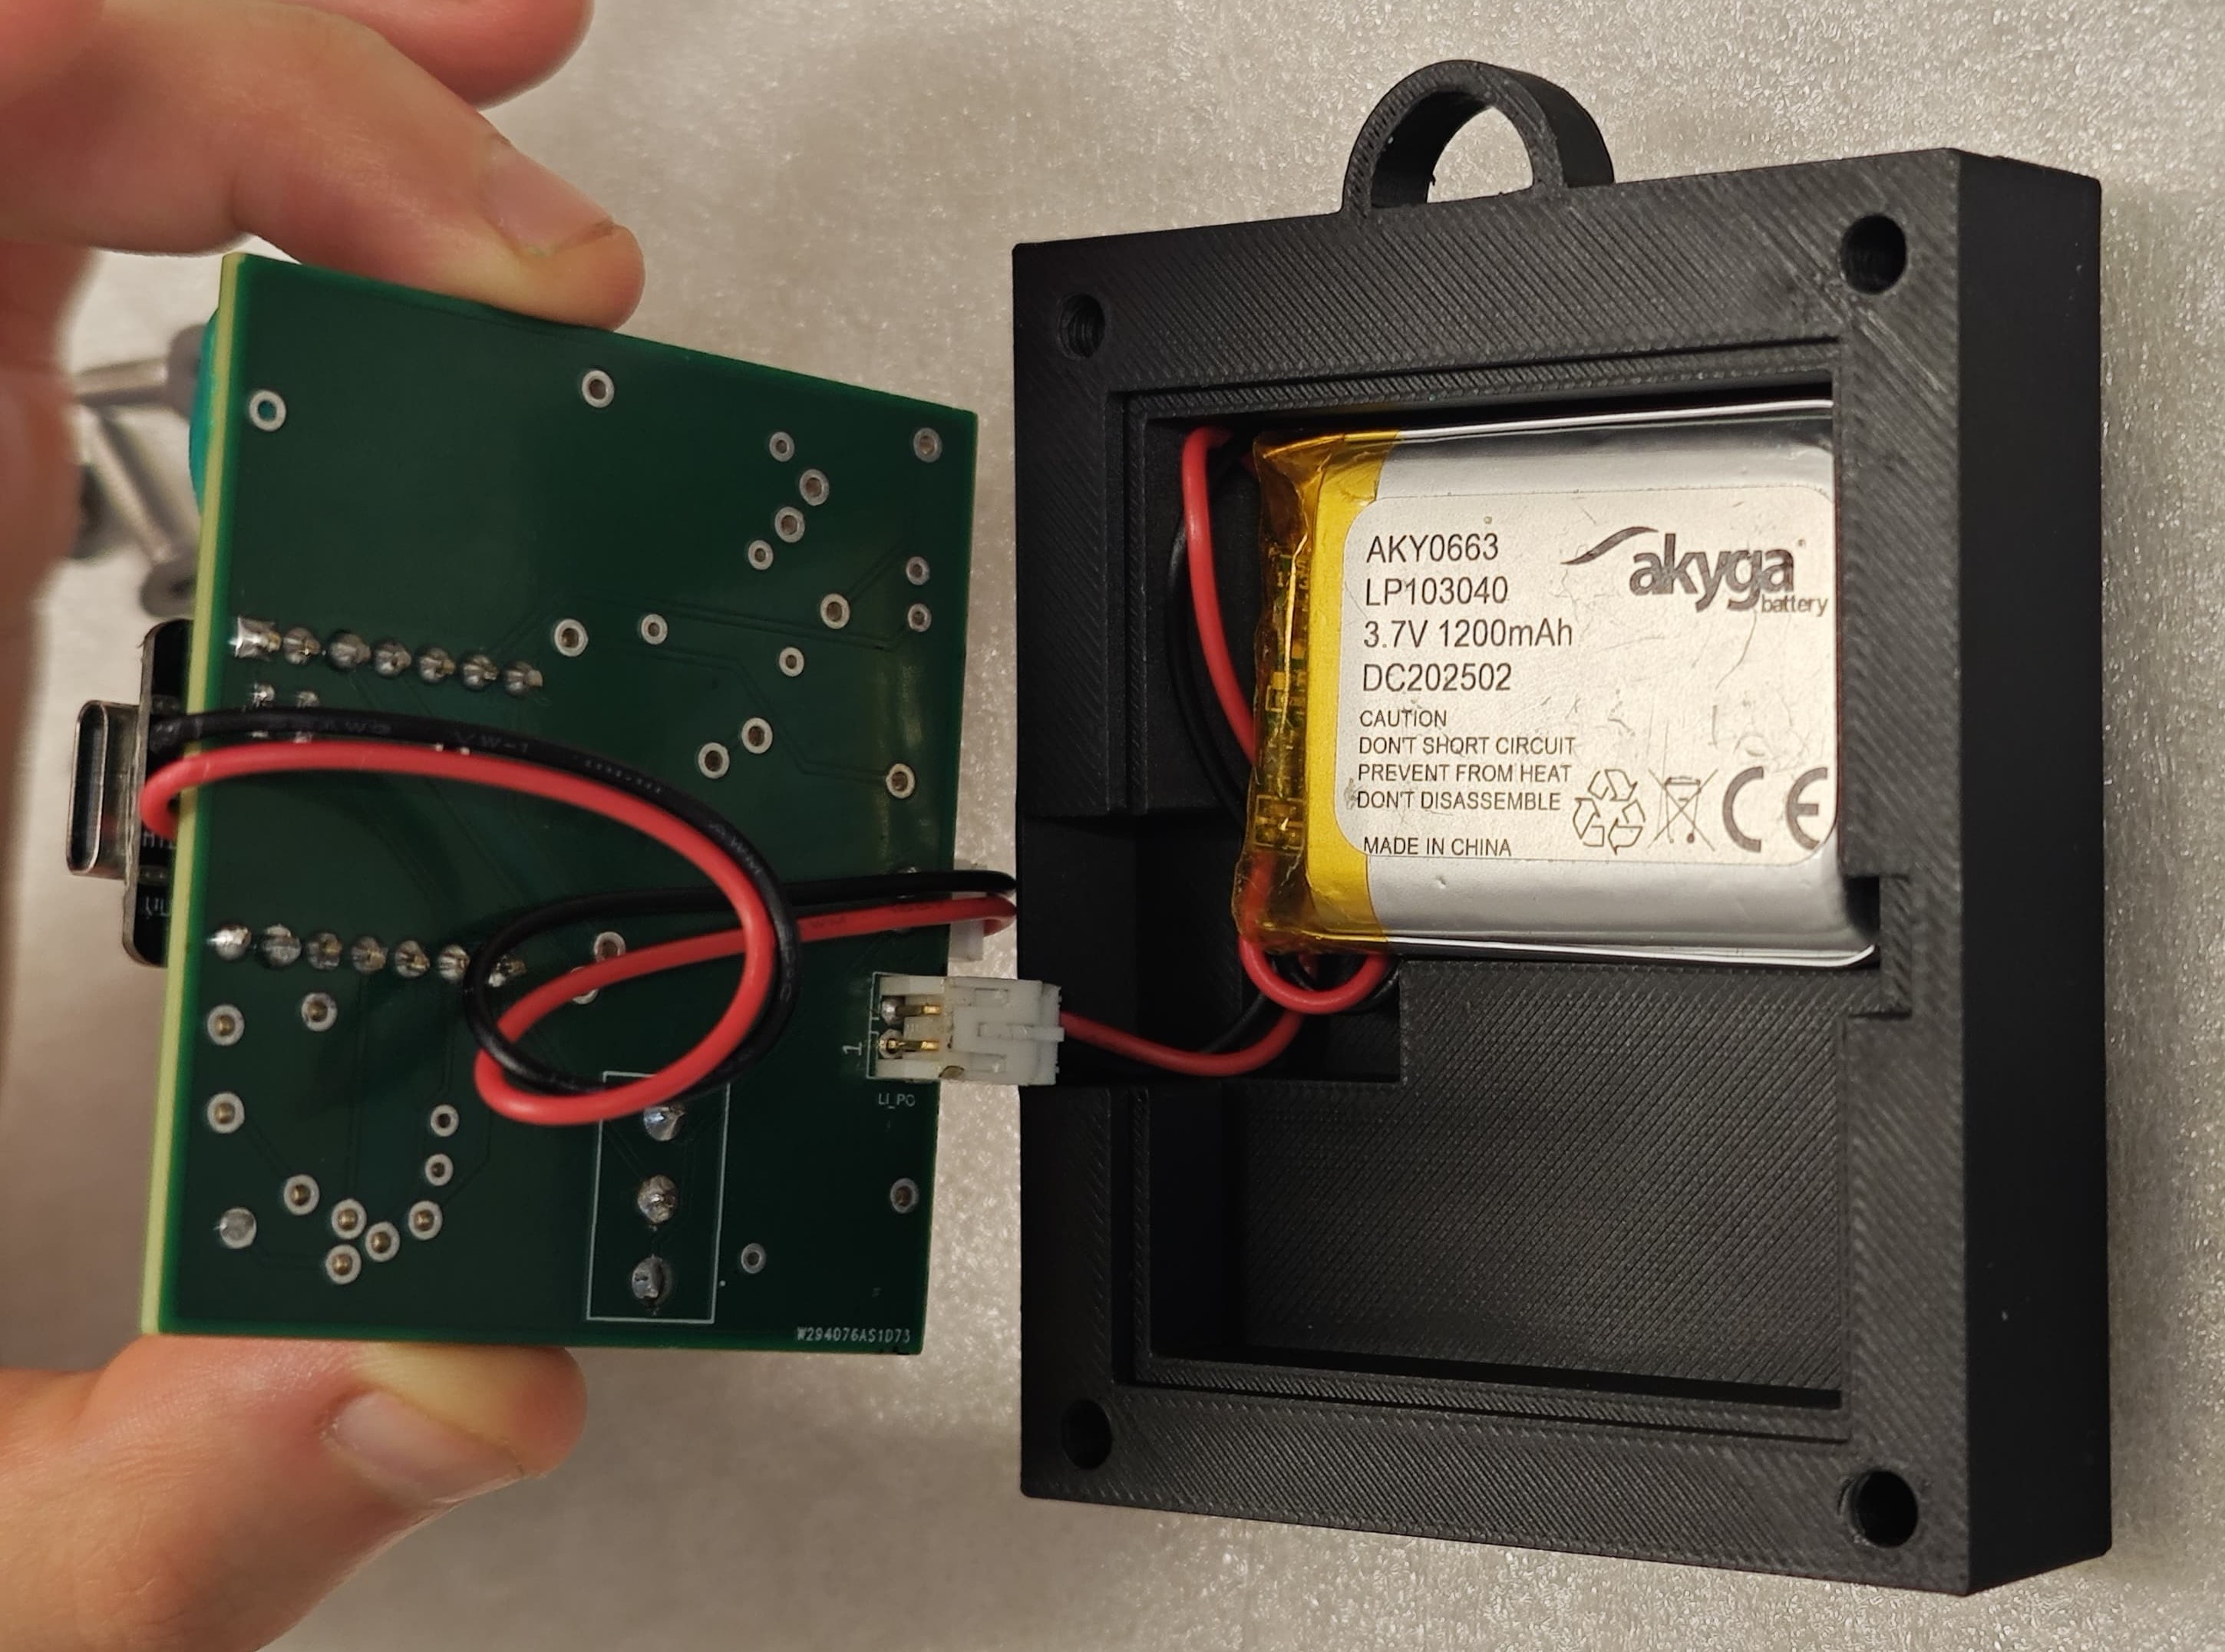
\includegraphics[width=177.75pt,height=136.9pt]{images/baixo.jpg}};

% ---- Battery + cables compartment ---------------------------------------
\node [lbl,draw={rgb, 255:red, 81; green, 81; blue, 81 },anchor=center]
      (batt) at (106.1,280.6) {Battery + Cables\\Compartment};
\draw [color={rgb, 255:red, 81; green, 81; blue, 81 },line width=1.1pt]
      ([xshift=12.5pt]batt.south) -- (147.0,240.4);
\draw [shift={(152.6,234.7)},rotate=134.3,ah,
       fill={rgb, 255:red, 81; green, 81; blue, 81 }]
      (7.85,-3.78) -- (0,0) -- (7.85,3.78) -- cycle ;

% ---- Power cables -------------------------------------------------------
\node [lbl,draw={rgb, 255:red, 241; green, 74; blue, 64 },anchor=center]
      (pcab) at (163.25,189.1) {Power\\Cables};
\draw [color={rgb, 255:red, 241; green, 74; blue, 64 },line width=1.1pt]
      ([xshift=-8pt]pcab.north) -- (151.0,213.7);
\draw [shift={(148.6,221.35)},rotate=287.4,ah,
       fill={rgb, 255:red, 241; green, 74; blue, 64 }]
      (7.85,-3.78) -- (0,0) -- (7.85,3.78) -- cycle ;
\draw [color={rgb, 255:red, 241; green, 74; blue, 64 },line width=1.1pt]
      ([xshift=-8pt]pcab.north) -- (126.4,217.7);
\draw [shift={(119.6,221.85)},rotate=328.6,ah,
       fill={rgb, 255:red, 241; green, 74; blue, 64 }]
      (7.85,-3.78) -- (0,0) -- (7.85,3.78) -- cycle ;

% ---- Panel letter (centred on the image) --------------------------------
\node [pan] at (148.375,164) {(a)};
\begin{scope}[yshift=8pt]
% =========================================================================
% (b)  middle shell  --  image x: 0 -> 135.7 , y: 0 -> 146
% =========================================================================
\node [anchor=south west,inner sep=0] at (0,0)
  {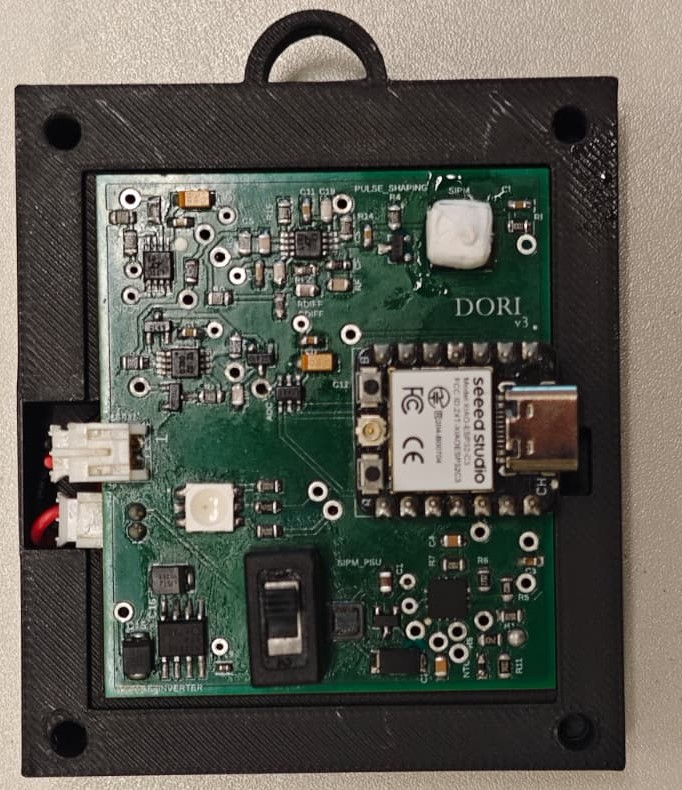
\includegraphics[width=135.7pt,height=146pt]{images/meio.jpg}};

% ---- Teflon-wrapped scintillator ---------------------------------------
\node [lbl,draw={rgb, 255:red, 26; green, 111; blue, 223 },anchor=center]
      (tefl) at (56.65,126.2) {Teflon-wrapped\\Scintillator};
\draw [color={rgb, 255:red, 26; green, 111; blue, 223 },line width=1.1pt]
      ([xshift=9.35pt]tefl.south) -- (79.2,107.0);
\draw [shift={(86.0,102.8)},rotate=148.2,ah,
       fill={rgb, 255:red, 26; green, 111; blue, 223 }]
      (7.85,-3.78) -- (0,0) -- (7.85,3.78) -- cycle ;

% ---- Width dimension (6.3 cm) ------------------------------------------
\draw [line width=1.1pt,black] (2,-4) -- (123.5,-4);
\draw [shift={(2,-4)},rotate=0,ah,fill=black]
      (7.85,-3.78) -- (0,0) -- (7.85,3.78) -- cycle ;
\draw [shift={(123.5,-4)},rotate=180,ah,fill=black]
      (7.85,-3.78) -- (0,0) -- (7.85,3.78) -- cycle ;
\node [dim,anchor=center] at (62.8,-4) {6.3~cm};
% ---- Height dimension (7.2 cm) -----------------------------------------
\draw [line width=1.1pt,black] (-4,3.5) -- (-4,132.5);
\draw [shift={(-4,3.5)},rotate=90,ah,fill=black]
      (7.85,-3.78) -- (0,0) -- (7.85,3.78) -- cycle ;
\draw [shift={(-4,132.5)},rotate=270,ah,fill=black]
      (7.85,-3.78) -- (0,0) -- (7.85,3.78) -- cycle ;
\node [dim,anchor=center,rotate=90] at (-4,68) {7.2~cm};

% ---- Panel letter -------------------------------------------------------
\node [pan] at (67.85,-10) {(b)};

% =========================================================================
% (c)  top shell  --  image x: 159.7 -> 296.8 , y: 0 -> 146
% =========================================================================
\node [anchor=south west,inner sep=0] at (159.7,0)
  {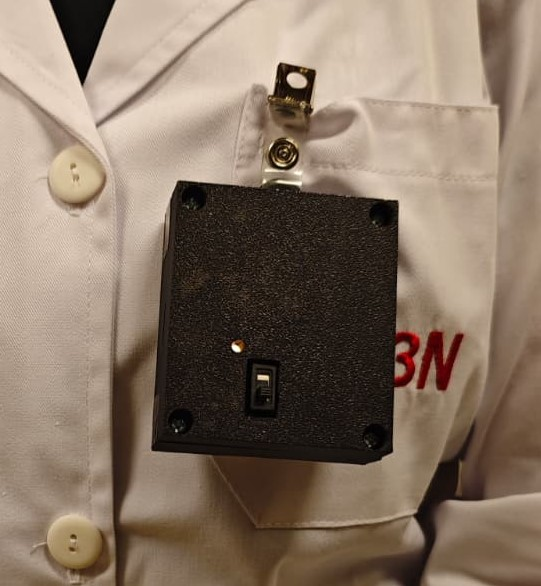
\includegraphics[width=137.1pt,height=146pt]{images/cima.jpg}};
% ---- LED --------------------------------------------------------------
\node [lbl,draw={rgb, 255:red, 204; green, 153; blue, 0 },anchor=center]
      (led) at (181.75,71.45) {LED On};
\draw [color={rgb, 255:red, 204; green, 153; blue, 0 },line width=1.1pt]
      (led.east) -- (217.6,61.6);
\draw [shift={(219.5,60.4)},rotate=151.2,ah,
       fill={rgb, 255:red, 204; green, 153; blue, 0 }]
      (7.85,-3.78) -- (0,0) -- (7.85,3.78) -- cycle ;
% ---- Badge clip ---------------------------------------------------------
\node [lbl,draw={rgb, 255:red, 55; green, 173; blue, 107 },anchor=center]
      (badge) at (269.4,107.7) {Badge Clip};
\draw [color={rgb, 255:red, 55; green, 173; blue, 107 },line width=1.1pt]
      (badge.north) -- (245.3,120.7);
\draw [shift={(237.5,122.6)},rotate=346.6,ah,
       fill={rgb, 255:red, 55; green, 173; blue, 107 }]
      (7.85,-3.78) -- (0,0) -- (7.85,3.78) -- cycle ;


% ---- Power switch -------------------------------------------------------
\node [lbl,draw={rgb, 255:red, 241; green, 74; blue, 64 },anchor=center]
      (psw) at (265.15,47) {Power\\Switch};
\draw [color={rgb, 255:red, 241; green, 74; blue, 64 },line width=1.1pt]
      (psw.west) -- (240,47);
\draw [shift={(232,47)},rotate=0,ah,
       fill={rgb, 255:red, 241; green, 74; blue, 64 }]
      (7.85,-3.78) -- (0,0) -- (7.85,3.78) -- cycle ;

% ---- Thickness dimension (2.5 cm, short arrow -> scaled heads) ----------
\draw [line width=1.1pt,black] (201.0,92.9) -- (205.8,101.6);
\draw [shift={(201.0,92.9)},rotate=61.1,ahs,fill=black]
      (7.85,-3.78) -- (0,0) -- (7.85,3.78) -- cycle ;
\draw [shift={(205.8,101.6)},rotate=241.1,ahs,fill=black]
      (7.85,-3.78) -- (0,0) -- (7.85,3.78) -- cycle ;
\node [dim,anchor=center,rotate=61] at (194.7,102.2) {2.5~cm};
% ---- Panel letter -------------------------------------------------------
\node [pan] at (228.25,-10) {(c)};
\end{scope}
\end{tikzpicture}}
  \caption[Final DORI prototype.]{Final DORI prototype. \textbf{(a)} Bottom layer of
the enclosure, with the compartment holding the LiPo battery and the cables that
connect it to the board. \textbf{(b)} Assembled PCB, with
the Teflon-wrapped scintillator coupled to the SiPM. \textbf{(c)} Closed prototype
worn over a lab coat, with the badge clip, the power switch and the LED on.}
  \label{fig:prototype}
\end{figure}

\section{Channel Response}
\label{sec:channel_response}

Although the readout circuit is the one described in Section~\ref{sec:front_end}, the response of the new prototype cannot be assumed to be that of the DORI-test board. Component values are specified within tolerance bands, and the parasitic contributions and noise coupling introduced by a board are a property of its layout. Both act on the final amplitude at the sampling stage, and consequently on the channel at which a given deposited energy is recorded. Characterising this response allows the front-end design to be treated as transferable and scalable to different board dimensions and formats. If the response of a new board can be related to that of the fully characterised DORI-test board, then the same readout can be used in whatever format each proposed monitoring position demands. 

To verify this, the \emph{Bremsstrahlung} endpoint procedure of Section~\ref{sec:energy_calibration} was repeated. Spectra were acquired over 5-minute intervals for tube voltages of 20 to 50~kVp, at tube currents of 0.100, 0.150 and 0.200~mA. The endpoint channel was extracted from each acquisition as before. The detector was again positioned within the beam line, although at a distance different from the one used previously. The change was required to prevent saturation of the front-end electronics across the full range of tube voltages, and it is the reason why no spectrum was obtained at 20~kVp. At this distance and fluence the counts registered at that voltage remain within the excluded background. A shorter distance or a higher tube current would recover the point at the cost of saturating the front end at the upper voltages. Additionally, the 3D printed case adds absorption, most significantly at the lower energies. The resulting endpoint channels are summarised in Table~\ref{tab:endpoints_prototype}. The uncertainty on the individual endpoints follows the pattern already described for the energy calibration. At 25~keV it is dominated by counting statistics, it decreases towards the middle of the interval. It increases again towards 50~keV, where photoelectric absorption in the scintillator drops and pile-up distorts the spectral shape near the abscissa.
% Requires \usepackage{tabularx} in the preamble

% Small vertical space after surrounding text
\vspace{1em}

% Manual table title, numbered and added to LoT
\refstepcounter{table}
\label{tab:endpoints_prototype}
\noindent\textbf{Table~\thetable.} \emph{Bremsstrahlung} endpoint channel for each tube voltage, obtained with the final prototype. Values are the mean of three acquisitions with the maximum deviation from the mean.
\addcontentsline{lot}{table}{\protect\numberline{\thetable}\emph{Bremsstrahlung} endpoint channel for each tube voltage, obtained with the final prototype.}

% Small space between title and table
\vspace{0.1em}

\begin{table}[H]
  \centering
  \begin{tabularx}{\textwidth}{>{\centering\arraybackslash}m{0.18\textwidth}
                               *{6}{>{\centering\arraybackslash}X}}
    \toprule
    \scriptsize \textbf{Tube Voltage (kVp)} & \scriptsize \textbf{25} & \scriptsize \textbf{30} & \scriptsize \textbf{35} & \scriptsize \textbf{40} & \scriptsize \textbf{45} & \scriptsize \textbf{50} \\
    \midrule
    \scriptsize \textbf{Endpoint Channel (a.u.)}
    & \scriptsize $30 \pm 4\%$
    & \scriptsize $34 \pm 1\%$
    & \scriptsize $36 \pm 1\%$
    & \scriptsize $39 \pm 1\%$
    & \scriptsize $41 \pm 1\%$
    & \scriptsize $42 \pm 2\%$ \\
    \bottomrule
  \end{tabularx}
\end{table}

 The endpoints obtained with the final prototype are presented against those of the test board at the same tube voltages in Fig.~\ref{fig:channel_response}. A linear fit was applied, and with $R^2 = 0.998$ a correspondence between the two boards can be expressed. The slope of the fit is $1.01 \pm 0.02$. This parameter translates the gain of the readout chain. If the two boards differed in gain, every channel would be scaled by a common factor, different from one, as the energy increased. The slope obtained is one within its uncertainty, so the gain is preserved on the new board, within the tolerance of the components that set it. The fit does not, however, pass through the origin. Comparing the endpoints of Tables~\ref{tab:endpoints_prototype} and~\ref{tab:endpoints} directly, the final prototype records every event $3.0 \pm 0.2$ channels below the test board, consistent with the intercept of the fit. With a unit slope, this displacement is the same at every energy of the interval. A difference that does not grow with the signal is additive, and corresponds to a baseline shift, in which all pulses are sampled from a level slightly lower than on the test board. With a channel width of 3.2~mV, three channels correspond to approximately 9.6~mV of shift, introduced at some point at the output of the shaper. The consequence for the calibration is direct as only the intercept changes. The slope of Eq.~\ref{eq:energy_conversion} is retained, since the gain is preserved, and $b$ is displaced by the constant offset. The calibration established for the DORI-test board therefore applies to the final prototype, and the energy of an event can be obtained from its channel simply through a conversion factor. Although the 20~kVp point could not be measured and the $^{241}$Am measurements were not repeated, the 20 to 60~keV range is still preserved, as long as the channels are corrected by the offset, as the response was shown to be linear in Section~\ref{sec:energy_calibration}.

 \begin{figure}[H]
  \centering
  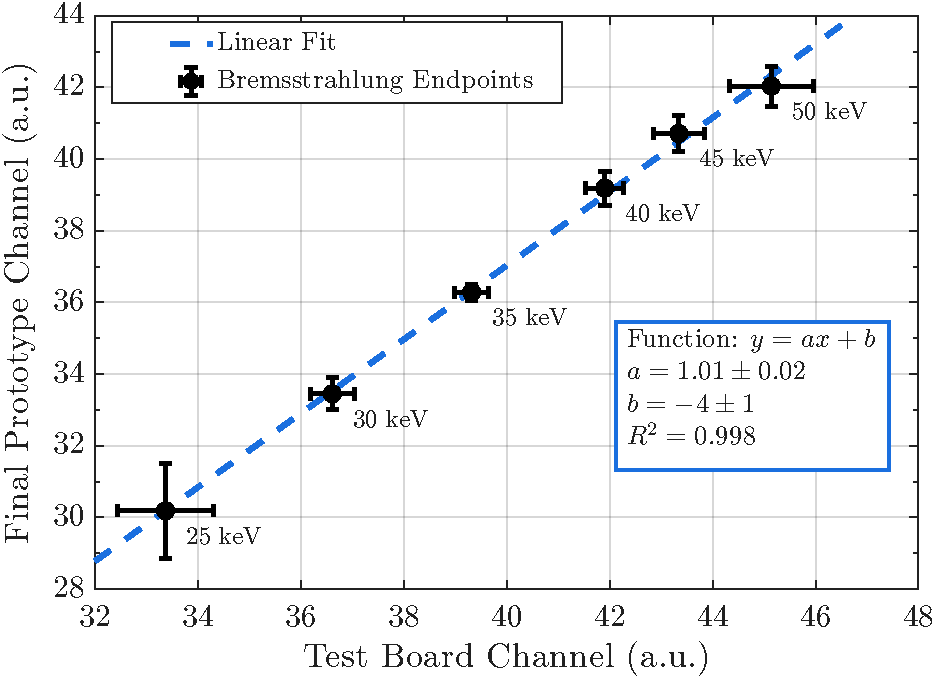
\includegraphics[width=0.85\linewidth]{images/channel_transfer.pdf}
  \caption[Endpoint channel correspondence between the DORI-test board and the final prototype.]{%
Linear fit of the \emph{Bremsstrahlung} endpoint channels recorded by the final
 prototype against those recorded by the DORI-test board, for the tube voltages common to both acquisitions.
  }
  \label{fig:channel_response}
\end{figure}


\section{Power Consumption}
\label{sec:power_consumption}
As a final test, and with a PCB optimised for wireless communication, the power consumption of the current DORI electronics and firmware was analysed. The battery was fully charged through the USB-C connector of the ESP32-C3, the end of the charge being indicated by the red LED of the MCU turning off, and a simulation firmware was
uploaded. One hundred interrupts (events) per second were simulated, and the battery voltage was read with \texttt{analogRead} through a voltage divider connected to the battery terminals. The event data were transmitted over BLE at a one second rate, and the battery voltage was recorded every 15 minutes. A cutoff was added at 3.3 V, at which the MCU is sent into deep sleep in order to preserve the LiPo cell from a full discharge. 

DORI operated for approximately 8.6 hours before the cutoff was reached, at a mean discharge rate of 80 mV/h. For the 1200 mAh cell used, this corresponds to a mean current of approximately 140 mA at 3.7 V. While this is sufficient for uninterrupted operation over an eight hour working day, it would require frequent charging cycles. Thefore, there is still room for improvement in the component selection of the DORI board with respect to consumption. Nevertheless, the battery voltage is a poor indicator of the charge remaining, and a proper characterisation of the cell would be required before it could be used to estimate the current state of charge.
Additionally, the integrity of the wireless link was kept intact throughout the run, with no disconnections and no lost notifications. No rise was registered in the temperature of the MCU, indicating that no thermal load builds up even after continuous hours of operation.

\section{Cost and Specifications}
\label{sec:cost_specifications}

DORI is also intended to represent a more cost effective solution against the prices currently charged for the active devices mentioned in the introduction. An estimated cost of the current prototype is listed in Table~\ref{tab:cost}, excluding assembly and the marginal cost of consumables. The detection chain accounts for most of the total, with the scintillator and the SiPM alone representing around 70\% of it. Even so, a finished product would still represent a fraction of the roughly 1000~dollars of a commercial device. The component selection can still be optimised, and at a larger production scale the cost per device is expected to fall further.

% Requires \usepackage{tabularx} and \usepackage{eurosym} in the preamble

\vspace{1em}
\refstepcounter{table}
\label{tab:cost}
\noindent\textbf{Table~\thetable.} Estimated cost of the components of the final DORI prototype as of September 2026.
\addcontentsline{lot}{table}{\protect\numberline{\thetable}Estimated cost of the components of the final DORI prototype.}

\vspace{0.1em}
\begin{table}[H]
  \centering
  \small
  \begin{tabularx}{0.55\textwidth}{>{\raggedright\arraybackslash}m{0.26\textwidth}
                                   >{\centering\arraybackslash}X}
    \toprule
    \textbf{Component} & \textbf{Cost (\euro)} \\
    \midrule
    BC-408 scintillator  & 110 \\
    SiPM                 & 50 \\
    Front-end components & $\sim$50 \\
    LiPo battery         & 7.40 \\
    PCB fabrication      & 5 \\
    XIAO ESP32-C3        & 4.25 \\
    3D printed enclosure & $\sim$2 \\
    \midrule
    \textbf{Total}       & \textbf{$\sim$229} \\
    \bottomrule
  \end{tabularx}
\end{table}
Finally, the characteristics of the final prototype, as established throughout this work, are summarised in Table~\ref{tab:specifications}.

\vspace{1em}

\refstepcounter{table}
\label{tab:specifications}
\noindent\textbf{Table~\thetable.} Specifications of the final DORI prototype.
\addcontentsline{lot}{table}{\protect\numberline{\thetable}Specifications of the final DORI prototype.}

\vspace{0.1em}

\begin{table}[H]
  \centering
  \small
  \renewcommand{\arraystretch}{1.25}
  \setlength{\tabcolsep}{3mm}
  \begin{tabularx}{0.65\textwidth}{|P|V|}
    \hline
    \textbf{Parameter} & \textbf{Value} \\
    \hline
    Dead time & 17.8 $\pm$ 0.4~$\mu$s \\
    \hline
    Calibrated energy range & 20 to 60~keV \\
    \hline
    Operational unit & $H_p(10)$ \\
    \hline
    % \newline, not \\, forces the second line: inside an X column \\
    % would end the table row.
    Calibrated dose range & N-25 to N-40 \newline
                            0.063 to 101~$\mu$Sv/h \\
    \hline
    Dimensions & 6.3 $\times$ 7.2 $\times$ 2.5~cm \\
    \hline
    Mass & 141~g \\
    \hline
    Autonomy & 8.6~h \\
    \hline
  \end{tabularx}
\end{table}
\chapter{Conclusions}

The readout is scalable.

Calibration to other depths (mainly Hp(3)) requires other phantoms!!!

The readout is ready to receive any scintillator, as long as the gain is adjusted.


\section{Future work}
Fix the residual baseline on the P\&H.

How can we get more calibration points up to 100–120 keV?

Where are these "certified laboratories"? aqui em Portugal (se houver)

BLE stability tests.




% The bibliography
%
%\cleardoublepage
%\iffalse

  \bibliographystyle{ieeetr}
  %\bibliographystyle{plain}
  {\footnotesize
\bibliography{Bibliografia}}
%\bibliography{Biblio}% replace by the name of name of your .bib file
%\cleardoublepage

% Appendix (chapters get lettered A, B, ... instead of numbered)
\appendix
\chapter*{Appendix}
\label{annex:sources}

% TODO (Marta): the May 2026 activities are filled in; still missing the serial
% numbers and the initial (certificate) activities for the three sealed sources used
% throughout the hardware/calibration chapters (referenced as "Annex~\ref{annex:sources}"
% from the Front-End Electronics section).

\section*{A - Sealed Source Activities}


\vspace{1em}
% Lettered to match the appendix sections (Table A, not Table 12), and deliberately
% kept out of the List of Tables: \thetable is redefined locally and the global table
% counter is put back afterwards, so the numbered tables in the chapters are unaffected.
\begingroup
\renewcommand{\thetable}{A}
\refstepcounter{table}\addtocounter{table}{-1}
\label{tab:sources}
\noindent\textbf{Table~\thetable.} Activity of the sealed sources used in this work.
\endgroup
\vspace{0.1em}

\begin{table}[H]
  \centering
  \renewcommand{\arraystretch}{1.4}
  \begin{tabular}{c c c c}
    \toprule
    \textbf{Source} & \textbf{Serial Number} & \textbf{Initial Activity} &
    \textbf{Activity in May 2026} \\
    \midrule
    $^{241}$Am & TODO & TODO & 23~kBq  \\
    $^{109}$Cd & TODO & TODO & 8.3~kBq \\
    $^{57}$Co  & TODO & TODO & 3.4~kBq \\
    \bottomrule
  \end{tabular}
\end{table}

\section*{B - BC-408 Photon Absorption in 5 mm}



\begin{figure}[H]
  \centering
  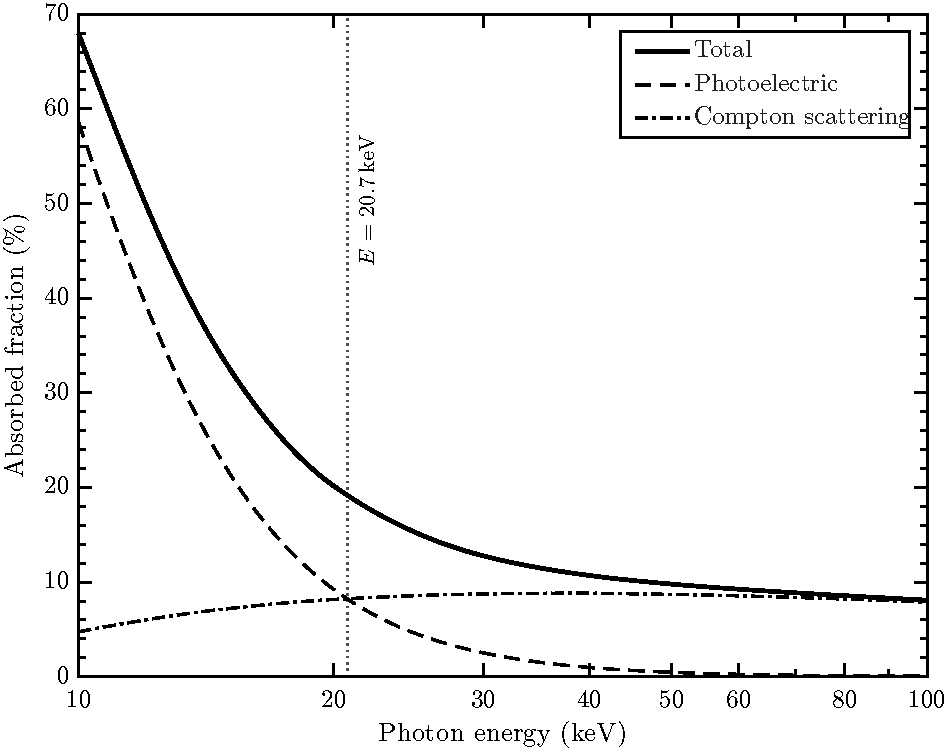
\includegraphics[width=\linewidth,height=0.5\textheight,keepaspectratio]{images/bc408.pdf}
  \label{fig:bc408}
\end{figure}

\end{document}
